% Thesis_Report_final.tex -- the final thesis report, written by the author.
% Chapter 1 (Introduction, from draft_main.tex) and Chapter 2 (Literature Review) carry full text; Chapters 3-7
% and the appendices are a skeleton: headings, labels and the figures to use. References for the writing:
% draft_main.tex (full draft, every final number) and main.tex (bullet guides, tables, equations).
\documentclass[11pt, a4paper]{report}

% --- Packages ---
\usepackage[utf8]{inputenc}
\usepackage[T1]{fontenc}
\usepackage{lmodern}
\usepackage{geometry}
\geometry{a4paper, margin=1in}
\usepackage{amsmath, amssymb, amsfonts}
\usepackage{booktabs}
\usepackage{float}
\usepackage{placeins}
\usepackage{graphicx}
\usepackage{caption}
\usepackage{array}
\usepackage{titlesec}
\usepackage{tabularx}
\usepackage{ragged2e}
\usepackage[table]{xcolor}
\usepackage{parskip}

% --- float placement: let figures and tables share pages with text (fewer half-empty float-only pages) ---
\renewcommand{\topfraction}{0.85}        % a float may fill up to 85 % of a page top
\renewcommand{\bottomfraction}{0.6}
\renewcommand{\textfraction}{0.12}       % a page needs only 12 % text to count as a text page
\renewcommand{\floatpagefraction}{0.8}   % a float-only page must be at least 80 % full
% wider page-number column in the contents and lists: appendix pages are roman (xxviii)
\makeatletter
\renewcommand{\@pnumwidth}{2.4em}
\renewcommand{\@tocrmarg}{3.2em}
\makeatother

% --- Document Info ---
\titleformat{\chapter}[hang]{\huge\bfseries}{\thechapter.\ }{0pt}{\huge\bfseries}
\titlespacing*{\chapter}{0pt}{-20pt}{20pt}
\title{State Space Models for Event-Based Object Detection: A Controlled Architectural Study with a Neuromorphic Deployment Path}
\author{Benas Vaiciulis}
\date{November 2026}

% --- running header and page style ---
\usepackage{fancyhdr}
\setlength{\headheight}{14pt}
\pagestyle{fancy}
\fancyhf{}
\fancyhead[L]{\small Benas Vaiciulis -- State Space Models for Event-Based Object Detection}
\fancyfoot[C]{\thepage}
\fancypagestyle{plain}{\fancyhf{}\fancyhead[L]{\small Benas Vaiciulis -- State Space Models for Event-Based Object Detection}\fancyfoot[C]{\thepage}}
\usepackage{hyperref}   % last

% Front and back matter are numbered in roman, the body in arabic, so the body's page count is the report length.
\newcounter{frontmatterpages}

% --- writing markers ---

% \tbd{...} marks prose still to be written. Set \tbdshowfalse before submission to hide
% every marker in one place (they will then render as nothing, and the document is clean).
% (xcolor is already loaded with the [table] option in the preamble above.)
\newif\iftbdshow \tbdshowtrue
\newcommand{\tbd}[1]{\iftbdshow{\color{red}\small\textbf{[TO WRITE: }\textit{#1}\textbf{]}}\fi}
\newcommand{\needsgpu}[1]{\iftbdshow{\color{orange!80!black}\small\textbf{[PENDING RUN: }\textit{#1}\textbf{]}}\fi}
% \res{...} marks a NUMBER awaiting a run. Unlike \tbd/\needsgpu it is never hidden by \tbdshowfalse, so a
% missing result cannot reach the submitted PDF silently. Search for \res{ to find every one.
\newcommand{\res}[1]{{\color{red}\textbf{[#1]}}}

\newcommand{\Dt}{$\Delta t$}
\begin{document}

% ===================================================================== FRONT MATTER (roman)
\pagenumbering{roman}

\begin{titlepage}
    \centering
    \vspace*{1cm}
    \Large\textbf{State Space Models for Event-Based Object Detection:}\\[4pt]
    \Large\textbf{A Controlled Architectural Study with a Neuromorphic Deployment Path} \\
    \vspace{0.5cm}
    \large Undergraduate Thesis\\
    Bachelor of Robotics and Mechatronic Engineering \\
    \vspace{1.5cm}
    \textbf{Author:} Benas Vaiciulis \\
    \textbf{Student zID:} z5457896 \\
    \textbf{Supervisor:} Dr Will Midgley \\
    \vspace{1.5cm}
    UNSW Sydney \\
    School of Mechanical and Manufacturing Engineering \\
    \vfill
    \textbf{Submitted:} November 20, 2026
\end{titlepage}

\chapter*{Originality Statement}
% TODO-Originality Statement
`I hereby declare that this submission is my own work and to the best of my knowledge it contains no materials previously published or written by another person, or substantial proportions of material which have been accepted for the award of any other degree or diploma at UNSW or any other educational institution, except where due acknowledgement is made in the thesis. Any contribution made to the research by others, with whom I have worked at UNSW or elsewhere, is explicitly acknowledged in the thesis. I also declare that the intellectual content of this thesis is the product of my own work, except to the extent that assistance from others in the project's design and conception or in style, presentation and linguistic expression is acknowledged.'

\chapter*{Use of Generative AI}
\addcontentsline{toc}{chapter}{Use of Generative AI}
% Check this statement against your own use of AI and the MMAN4953 / UNSW rules before submitting;
% add any other AI tool you used.
I used the generative AI assistant Claude (Anthropic), throughout this project. I wrote the code, set the direction of the work, made the research decisions in discussion
with my supervisor, ran the training and evaluation runs, and reviewed the outputs. The assistant helped with
the following parts of the work:
\begin{itemize}
  \item \textbf{Software:} helping me debug my code and write the automated tests.
  \item \textbf{Literature:} searching for and summarising papers, and checking published numbers against the
        original papers.
  \item \textbf{Report structure:} planning the chapter and section structure and the order of headings.
  \item \textbf{Tables and figures:} writing the LaTeX tables and the scripts that draw the figures from my own
        logged results. All data shown come
        from my own experiments.
  \item \textbf{LaTeX:} finding and fixing LaTeX errors and layout problems.
  \item \textbf{Language:} Fixing grammatical errors and language style.
\end{itemize}

The research direction, the decisions on which experiments to run, and the judgement on the claims
are mine. Every number in the tables and figures was checked against the original result files, and I take
full responsibility for the content of this thesis.

\chapter*{Abstract}
\addcontentsline{toc}{chapter}{Abstract}
Event cameras report changes in brightness at each pixel as they happen, with microsecond timing and a very
wide brightness range. This makes them ideal for small drones, which have little space for weight or power
for computing. State space models, a type of neural network that processes long sequences efficiently, have
recently been proposed for event data. However, published comparisons change several parts of the detector
at once, so it is unclear what the state space model itself contributes. This thesis isolates that. It first
reproduces the published S5-RVT detector exactly, at 47.7 mean average precision (mAP) on the Gen1 driving
dataset. It then builds two new detectors on the same pipeline that differ only in how they combine
information across the image. EventSSM uses a convolutional network, and PureSSM a state space model. They
score 46.2 and 46.4~mAP, which is effectively equal, but PureSSM is the smallest model, needs the least
computation and scores 2.95 points higher on large objects. A receptive-field analysis shows
that it learns to draw on an area of the image up to twice as wide. When frames arrive ten times faster than
in training, the state space models keep 62 to 70\,\% of their accuracy, but a ConvLSTM detector keeps
80\,\%. Rescaling the step size $\Delta$ at test time, the correction proposed for this case, lowered accuracy by
9 to 13 points and the reported 39.84~mAP at ten times the rate could not be
reproduced with the released code and model. None of the models are best at everything. Finally, a spiking version of PureSSM splits the cost of spiking into three
parts. The neuron's leak and reset cost 0.3 points, sparsity (most outputs being zero) 1.5 points, and reducing each signal to a single bit 0.5 points.
With full training, the graded version comes within 0.2 points of PureSSM. Because its spikes reach only about 1\,\% of the detector's operations,
its estimated energy saving is below 1\,\%. Larger savings would require the spatial part of the network to
spike as well. A clear benefit of SSMs for event driven object detection is therefore a wider spatial context at lower compute cost.

\chapter*{Acknowledgements}
\addcontentsline{toc}{chapter}{Acknowledgements}
% TODO-Acknowledgements
The author gratefully acknowledges the guidance and support of Will Midgley in shaping the direction of
this research. Thanks are also extended to the staff of the School of Mechanical and Manufacturing
Engineering at UNSW Sydney for their support.

\tableofcontents
\clearpage\phantomsection\addcontentsline{toc}{chapter}{\listfigurename}
\listoffigures
\clearpage\phantomsection\addcontentsline{toc}{chapter}{\listtablename}
\listoftables

\chapter*{Nomenclature}
\addcontentsline{toc}{chapter}{Nomenclature}
\begin{tabular}{ll}
\multicolumn{2}{l}{\textbf{Latin Symbols}} \\[4pt]
$A$ & state transition matrix \\
$\bar{A}$ & discretised state matrix \\
$B$ & input projection matrix \\
$\bar{B}$ & discretised input matrix \\
$C$ & contrast threshold \\
$C_{ssm}$ & SSM output projection matrix \\
$d_{model}$ & model embedding dimension \\
$h(t)$ & hidden state vector (continuous time) \\
$h(k)$ & latent state vector at discrete step $k$ \\
$L(x,y,t)$ & log luminance \\
$P$ & event polarity (+1 or -1) \\
$I$ & identity matrix \\
$t$ & time, s \\
$u(t)$ & input signal \\
$x, y$ & pixel coordinates \\[8pt]
\multicolumn{2}{l}{\textbf{Greek Symbols}} \\[4pt]
$\Delta$ & SSM discretisation step size \\
$\Delta_t$ & step size at time $t$ (Mamba, depends on the input) \\[8pt]
\multicolumn{2}{l}{\textbf{Acronyms}} \\[4pt]
CNN & Convolutional Neural Network \\
DAVIS & Dynamic and Active-pixel Vision Sensor \\
DVS & Dynamic Vision Sensor \\
EST & Event Spike Tensor \\
GNN & Graph Neural Network \\
HDR & High Dynamic Range \\
LIF & Leaky Integrate-and-Fire \\
LTI & Linear Time-Invariant \\
RNN & Recurrent Neural Network \\
SNN & Spiking Neural Network \\
SSM & State Space Model \\
SSD & Single Shot MultiBox Detector \\
SWaP & Size, Weight, and Power \\
AP & Average Precision \\
BPTT & Backpropagation Through Time \\
ERF & Effective Receptive Field \\
FPN & Feature Pyramid Network \\
INRC & Intel Neuromorphic Research Community \\
IoU & Intersection over Union \\
mAP & mean Average Precision \\
NIR & Neuromorphic Intermediate Representation \\
PAFPN & Path Aggregation Feature Pyramid Network \\
SOP & Synaptic Operation \\
TBPTT & Truncated Backpropagation Through Time \\
UAV & Unmanned Aerial Vehicle \\
\end{tabular}

% ===================================================================== BODY (arabic, target about 50 pages)
\clearpage
\setcounter{frontmatterpages}{\value{page}}
\pagenumbering{arabic}

% ===================================================================== CHAPTER 1 (full text, from draft_main.tex)
\chapter{Introduction}
\label{ch:intro}
Micro unmanned aerial vehicles (UAVs) are widely used for infrastructure inspection, search and rescue, indoor and outdoor mapping, and environmental monitoring \cite{floreano2015science}. Under Australian regulation, micro UAVs are remotely piloted aircraft of at most 250 grams \cite{casa2021part101}. Their small size lets them enter tight spaces, perform agile manoeuvres and carry out search-and-rescue missions in places that larger aircraft cannot reach. However, their size also limits their payload capacity, onboard computing and power budget. These size, weight and power (SWaP) limits are a core engineering challenge for both the software and the hardware of autonomous drones.

Conventional frame cameras are widely used, mature and well supported by deep neural network frameworks. Like any technology, they have limitations, particularly for UAV flight. A frame camera captures the whole image at a fixed rate, so much of each frame is redundant. Frame cameras also suffer from motion blur at high speed and have a limited dynamic range. Event cameras, also known as dynamic vision sensors (DVS), work differently. Each pixel is independent and asynchronous. It responds to changes in log luminance and produces a stream of events with microsecond temporal resolution and a dynamic range above 120 dB \cite{gallego2020event}. Because each pixel reports changes as they happen, event cameras show very little motion blur \cite{gallego2020event}. Agile UAVs must detect obstacles at high speed, process the information and then avoid the obstacle. The low latency of event cameras makes this possible: early studies of event-based obstacle avoidance \cite{falanga2020dynamic, sanket2020evdodgenet} report perception latencies as low as 3.5 milliseconds \cite{falanga2020dynamic}.

While the sensors have matured, algorithms suited to event streams have lagged behind. Most approaches convert the asynchronous event stream into fixed time windows, packaged as frame-like inputs for convolutional neural networks (CNNs) or recurrent neural networks (RNNs) \cite{gehrig2019end, gehrig2023recurrent}. This packaging discards much of the fine timing that makes event cameras unique, so the input starts to resemble that of an ordinary camera. Transformer architectures, commonly used in large language models (LLMs), can model long-range dependencies, but their computational cost grows quadratically with the input length \cite{vaswani2017attention}. This cost weighs heavily on the resource-constrained processors typical of micro-UAVs.

State space models (SSMs), including the recent Mamba architecture and its variants \cite{gu2023mamba, dao2024transformers}, offer a promising alternative. Unlike CNNs, RNNs and transformers, SSMs model an input sequence as a continuous-time linear dynamical system, which can be discretised at different time steps. Their cost grows only linearly with sequence length, while they keep strong temporal reasoning \cite{gu2023mamba, gu2022efficiently}. Zubi\'{c} et al.~\cite{zubic2024state} recently reported that SSMs handle the variable temporal resolution of event-driven data, degrading far less than RNN- or transformer-based models when run at inference frequencies other than the training frequency. This thesis therefore investigates SSMs for event-based object detection, motivated by the perception needs of agile micro-UAVs. Obstacle avoidance became the motivating application (Section~\ref{sec:scope}).
\newpage
\section{Research Question and Aims}
\label{sec:rq}
Prior work establishes that state space models are competitive on event-camera detection, but
every published comparison changes several things at once (backbone, tokeniser and training recipe together), so the contribution of the sequence model itself cannot be read off the result. This
thesis narrows the question:

\begin{quote}
\textbf{Holding the entire detection pipeline fixed, what is the isolated effect of the backbone's
spatial mixer, on accuracy, temporal robustness and efficiency
for event-based object detection?}
\end{quote}

A second question motivates the neuromorphic strand of the work. What does it cost to make such a detector spiking, and what does neuromorphic hardware give back
in return?

To answer these questions, this thesis sets six aims:
\begin{enumerate}
  \item Reproduce the published S5-RVT detector and confirm that it reaches its reported accuracy of
        47.7~mAP.
  \item Build two new detectors, EventSSM and PureSSM, and compare their accuracy overall, for each object class and for each object size.
  \item Explain why any difference in accuracy occurs.
  \item Measure how well the detectors cope when the rate of incoming events changes, and compare them with a published ConvLSTM detector on
        the same test data.
  \item Measure model efficiency through model size, computational requirements, inference speed, energy consumption and memory use, using metrics relevant to future deployment on resource-constrained platforms.
  \item Build a spiking version of the detector and break down the accuracy it loses into separate costs.
\end{enumerate}
These aims refine the aims in Thesis~A. The Thesis~A aim of connecting the detector to an
obstacle-avoidance controller was later removed from the scope, as explained in
Section~\ref{sec:scope_change} and summarised in Table~\ref{tab:aims}.

\section{Hypotheses}
\label{sec:hypotheses}
The aims lead to four testable hypotheses:
\begin{description}
  \item[H1 Large objects.] A state space model used as the spatial mixer can draw on a wider area
            of the image than a convolutional network, so PureSSM should detect large objects better than
            EventSSM (Sections~\ref{sec:acc_results} and~\ref{sec:erf}).
  \item[H2 Changes in event rate.] State space models should stay accurate when events arrive
            faster than in training, and lose less accuracy than a ConvLSTM detector, as
            Zubi\'{c} et al.~\cite{zubic2024state} report (Section~\ref{sec:robustness}).
  \item[H3 The published correction.] Adjusting the state space model's time step to the new event
            rate, as Zubi\'{c} et al.\ propose, should make the models more robust still
            (Section~\ref{subsec:f2}).
  \item[H4 The cost of spiking.] Among the three spiking versions of the detector, the analog
            version should be at least as accurate as the graded version, and the graded version more
            accurate than the binary version (Section~\ref{subsec:spk_ladder}). 
\end{description}

\section{Contributions}
\label{sec:contributions}
The thesis makes seven contributions.
\begin{enumerate}
      \item A reproduction study of the time-step correction. Applied in the thesis with the published code and model, the
        correction reported to make state space models more robust to faster event rates lowers accuracy at every
        point tested, by 9 to 13~mAP at ten times the rate, and the published 200-Hz result could not be
        reproduced. The robustness itself is achieved without the correction. A published ConvLSTM
        detector, tested on the same data, is more robust than every state space model.
\item A breakdown of the cost of spiking. A hybrid spiking version of PureSSM whose temporal
        readout has three modes sharing one neuron model. Analog, graded and spike. Stepping from PureSSM
        through the three modes separates the accuracy cost of the neuron's leak and reset, sparsity and of the single bit ($-0.28$, $-1.52$ and $-0.54$~mAP on a common 100k-step schedule, and the intervals
        of the last two exclude zero). Published spiking detectors report at most one difference between a
        spiking and a non-spiking model. On the full schedule, the graded readout reaches 46.24~mAP against
        PureSSM's 46.43.
  \item A verified starting point. An exact reproduction of the published S5-RVT detector
        (47.7~mAP on the Gen1 test set), so that every later comparison rests on checked data preparation
        and evaluation code.
  \item Two new detectors in a controlled comparison. EventSSM and PureSSM, built by replacing only
        the backbone of that pipeline. They differ only in their spatial mixer and in pre-training, and the
        spiking variant differs from PureSSM only in its temporal readout, so each difference can be traced
        to one part of the detector.
  \item An explanation of the large-object result. A receptive-field probe shows that the state
        space mixer learns to draw on an area of the image up to twice as wide as the convolutional one, and
        that training widens it. This fits PureSSM's gain on large objects.
  \item A complete efficiency comparison. Four detectors, including the ConvLSTM, measured for size,
        computation, speed, energy and memory on one graphics card. The results that do not favour the new
        models. PureSSM is the slowest in normal mode, and the Mamba models need 31 times
        more memory per video stream.
  \item A mapped path to neuromorphic hardware. A spiking readout built for the graded spikes of
        Loihi~2, its measured activity and estimated energy, a NumPy reference version of the spiking
        temporal block, and an ordered route from the simulated model to the chip
        (Section~\ref{sec:neuro_case}).
\end{enumerate}

\section{Scope}
\label{sec:scope}
Thesis~A included an additional aim, the integration of the detector with an
obstacle-avoidance controller in simulation, and physical micro-UAV testing if feasible. That
aim was descoped, and the effort was redirected into the controlled architectural study and the
neuromorphic path. Section~\ref{sec:scope_change} states the justification for this change.
The SWaP motivation for the work is unchanged.

\section{Thesis Organisation}
\label{sec:organisation}
Thesis is organised as follows. Chapter~\ref{ch:lit} reviews the literature on event cameras
and how their data is represented, detection methods, state space models, spiking networks and
neuromorphic hardware. It ends with the research gaps that the thesis addresses.

Chapter~\ref{ch:method} describes how the detectors were built, trained and tested. It covers the input, the shared
detection pipeline, the five models, the dataset and how each result was measured.
Chapter~\ref{ch:results} reports the results, from the baseline reproduction, accuracy and its explanation, robustness to the event rate, efficiency and example detections to the spiking model.

Chapter~\ref{ch:discussion} explains what the results mean. It also sets out the path to neuromorphic hardware, and discusses the change of scope, the
limitations and future research. Chapter~\ref{ch:conclusion} is the conclusion.

The appendices give the mathematical details (Appendix~\ref{app:maths}), what is needed to reproduce the
results (Appendix~\ref{app:repro}), the project timeline (Appendix~\ref{app:timeline}), the risk assessment
(Appendix~\ref{app:risk}) and further results (Appendix~\ref{app:extra}).

% ===================================================================== CHAPTER 2 (full text)
\chapter{Literature Review}
\label{ch:lit}

\section{Event-Based Cameras: Principles and Hardware}
Event-based cameras, or neuromorphic vision sensors, work differently from conventional frame-based cameras. Rather than capturing synchronous frames at a fixed rate, each pixel independently monitors changes in log luminance and asynchronously spikes an event when the change exceeds a defined threshold $C$ (Figure~\ref{fig:dvs_principle}). A pixel at coordinates $(x, y)$ generates an event $e = (x, y, t, p)$ at time $t$ when $|L(x, y, t) - L(x, y, t - \Delta t)| \geq C$, where $L$ denotes log luminance and $p \in \{+1, -1\}$ indicates the polarity of the brightness change \cite{gallego2020event}, \cite{lichtsteiner2008128x128}. This principle is modelled on the ganglion cells of the retina, it gives several advantages over frame-based imaging like microsecond temporal resolution (typically 1 µs), very high dynamic range (>120 dB), low latency, low power consumption, and the little to none motion blur \cite{gallego2020event}.

Gallego et al.~\cite{gallego2020event} surveyed event-based vision, reviewing the development of neuromorphic sensors from the original silicon retina proposed by Mahowald and Mead in 1992 through to modern commercially available sensors. The Dynamic Vision Sensor (DVS), developed at ETH Zurich, was among the first widely adopted event cameras and demonstrated the feasibility of asynchronous vision for robotics applications \cite{lichtsteiner2008128x128}. The next step was the Dynamic and Active-pixel Vision Sensor (DAVIS), which combines a DVS with a conventional active pixel sensor on the same die, enabling simultaneous capture of events and intensity frames at the same pixel locations \cite{brandli2014240x180}.

Prophesee has developed a series of commercial event cameras with increasing resolution and performance. The Gen3.1 sensors, used in the DSEC dataset \cite{gehrig2021dsec}, offer VGA-resolution event sensing, while the latest IMX636 sensor, developed in collaboration with Sony, provides 1280×720 HD resolution with ultra-high-speed operation \cite{prophesee2026metavision}. At the opposite end of the spectrum, the GenX320 sensor targets ultra-low-power applications with a 320×320 pixel array drawing about 3\,mW in typical operation and as little as 36\,$\mu$W in its lowest-power mode, making it ideal for resource-constrained micro UAV platforms \cite{prophesee2025genx320}.

Current event cameras still have a lower spatial resolution than frame-based cameras. While modern frame-based sensors routinely achieve multi-megapixel resolutions, event cameras remain in the VGA to HD range. Event cameras also produce no output in static scenes, which can be both an advantage (data efficiency) and a limitation (loss of static information). Algorithms must therefore use the timing information of event cameras while working around their lower resolution.

\begin{figure}[htbp]
    \centering
    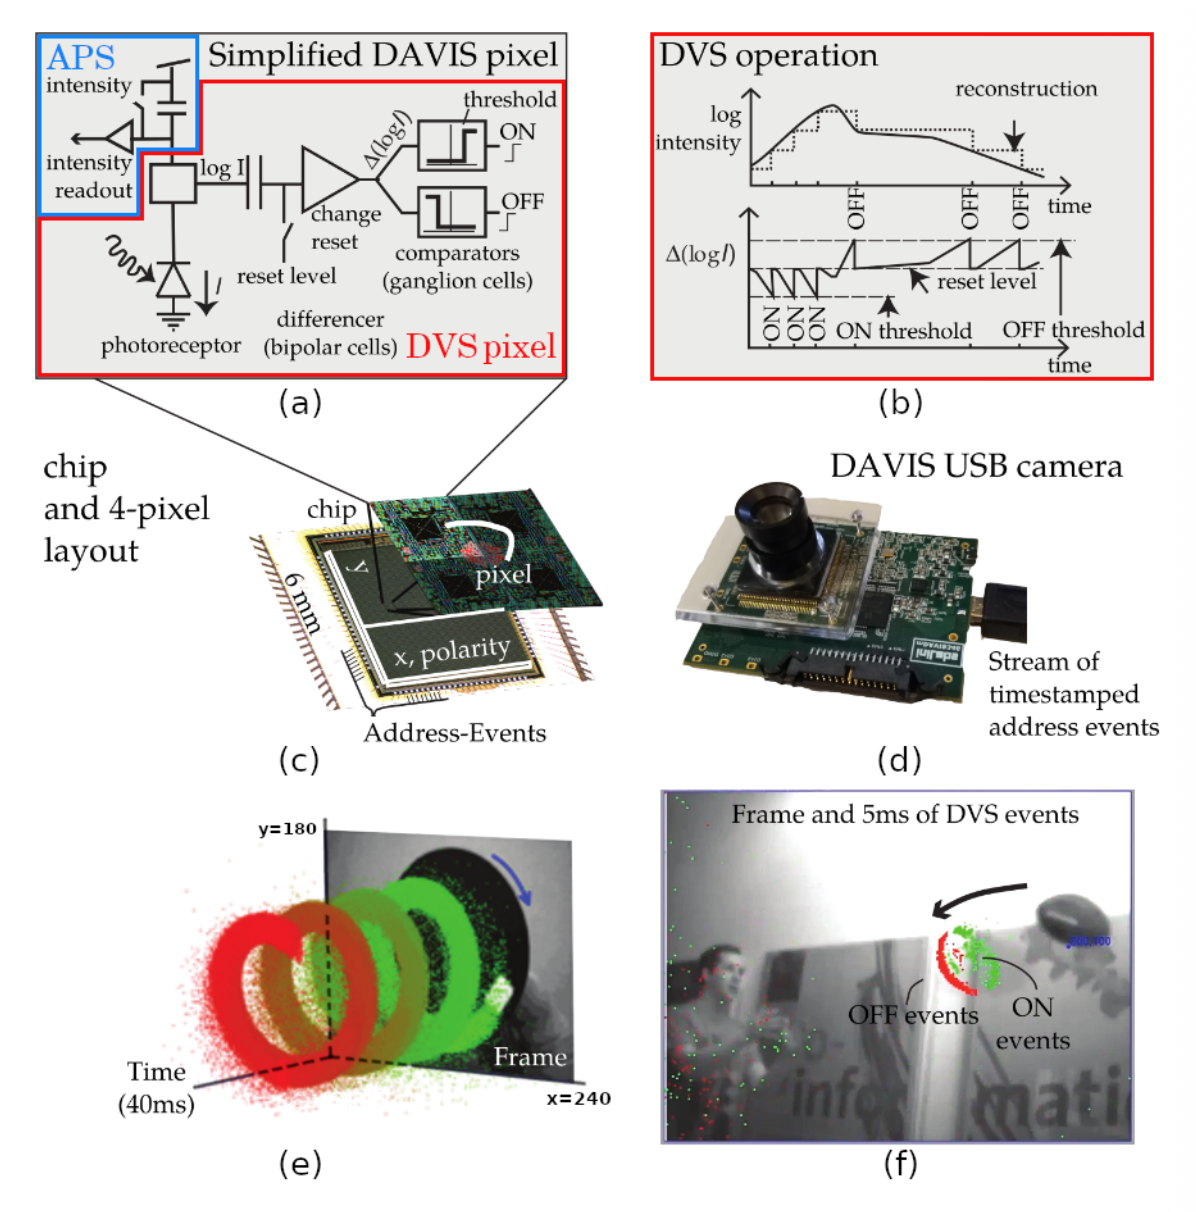
\includegraphics[width=0.75\textwidth]{images/fig_event_camera_principle.png}
    \caption[How an event camera works]{How an event camera works. Each pixel reports an event $(x, y, t, p)$ on its own whenever its brightness
        changes by more than a threshold $C$. Adapted from \cite{gallego2020event}.}
    \label{fig:dvs_principle}
\end{figure}

\section{Event Representations for Deep Learning}
Deep learning models expect dense tensors of fixed size. An event camera delivers a sparse, asynchronous stream of events instead.

The simplest representation is the event frame or event histogram, which accumulates events within a fixed time window into a two-dimensional grid where each pixel takes a value in {+1, 0, -1} based on event polarity \cite{gallego2020event}. While this representation is directly compatible with standard CNN architectures, it discards temporal information within the accumulation window, reducing the event stream to a snapshot that loses the fine timing that distinguishes event cameras from conventional sensors.

Voxel grids, proposed by Zhu et al.~\cite{zhu2019unsupervised}, address this limitation by discretising the event stream into a three-dimensional spatio-temporal volume. Events are accumulated into B temporal bins, producing a tensor of dimensions B × H × W that preserves temporal ordering (Figure~\ref{fig:voxel_grid}). This representation has been adopted in past work, including the Events-to-Video (E2VID) reconstruction framework \cite{rebecq2019e2vid} and various optical flow estimation methods. The number of temporal bins B represents a tuneable parameter balancing temporal resolution against computational cost.

\begin{figure}[htbp]
    \centering
    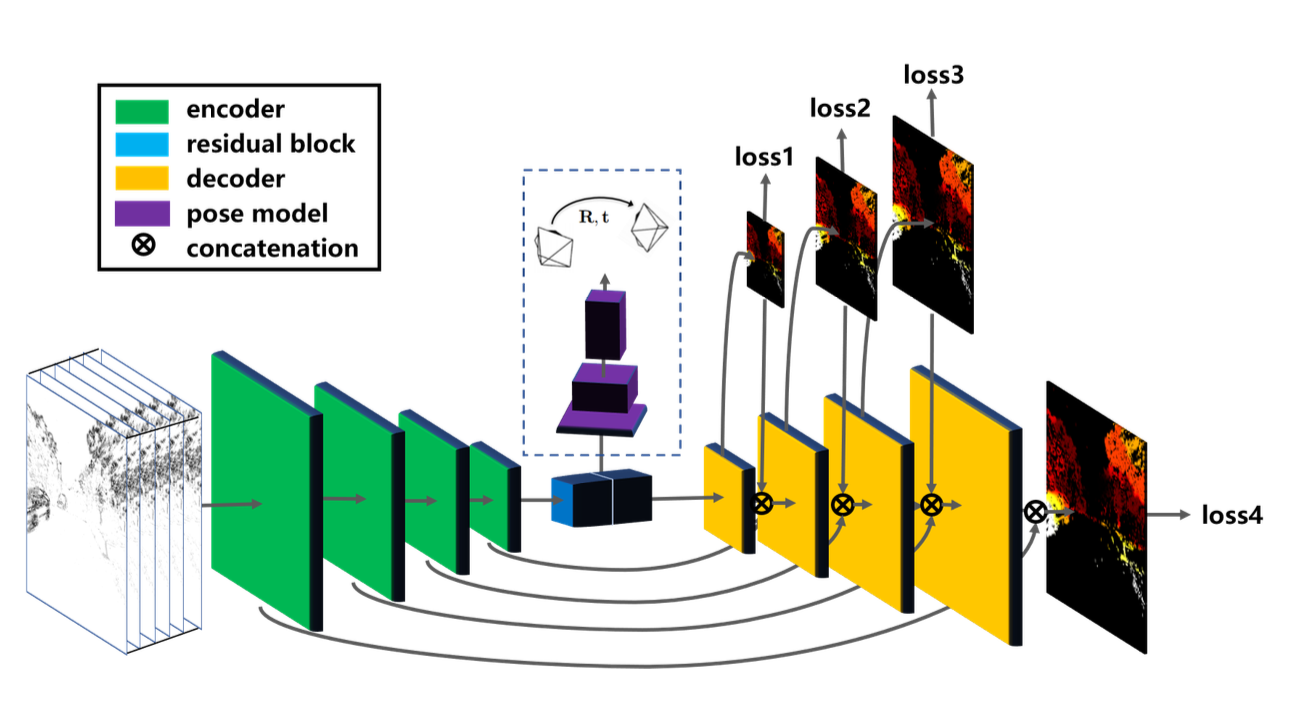
\includegraphics[width=0.75\textwidth]{images/fig_voxel_grid.png}
    \caption[Voxel grid event representation]{A voxel grid: the events of a time window are sorted into $B$ time bins, giving a $B \times H \times W$
        input. Adapted from \cite{zhu2019unsupervised}.}
    \label{fig:voxel_grid}
\end{figure}

Time surfaces, introduced by Lagorce et al.~\cite{lagorce2017hots}, offer an alternative encoding where each pixel stores an exponentially decaying function of the time since the last event at that location. This representation naturally encodes recency information and has been extended to Speed-Invariant Time Surfaces (SITS) that normalise for object velocity \cite{manderscheid2019speed}. Time surfaces are particularly effective for feature extraction and pattern recognition tasks, as they encode both spatial structure and temporal dynamics in a compact two-dimensional representation.

Event Spike Tensors (ESTs), proposed by Gehrig et al.~\cite{gehrig2019end}, sample the event stream using learned kernel functions, preserving temporal localisation with minimal information loss. Comparative studies have consistently demonstrated that representations retaining temporal localisation, such as voxel grids and ESTs, outperform simpler aggregation methods like event frames on downstream tasks \cite{gehrig2019end}. This shows that preserving the fine timing of events matters.

More recently, hybrid representations combining multiple channels of information have been explored. For instance, the Temporal Binary Representation packs the presence of events in successive sub-intervals into the bits of a single frame and has improved event-based action recognition \cite{innocenti2021temporal}. The best representation often depends on the task.

This thesis uses the stacked histogram of RVT \cite{gehrig2023recurrent}, which counts the events of each 50-ms window in ten temporal bins for each of the two polarities (Appendix~\ref{subsec:stacked_hist}). Like a voxel grid it preserves temporal ordering across bins, a property shown to matter for detection performance \cite{gehrig2019end}, and it is directly compatible with standard CNN and SSM-based backbones. It was not selected by a fresh comparison. It is part of the verified baseline's frozen pipeline (Section~\ref{sec:frozen_pipeline}), and changing it would confound the backbone comparison that is the subject of this thesis. The voxel grid proposed in the Thesis~A plan was therefore not adopted. Time surfaces, although compact, collapse temporal structure into a single 2D map and are less suited to multi-object detection tasks where simultaneous events at different locations must be disambiguated. ESTs offer higher temporal fidelity through learned kernels, but introduce additional parameters and training complexity that is difficult to justify given the computational constraints of onboard UAV deployment.

Compact multi-channel encodings of this kind have shown promise for action recognition \cite{innocenti2021temporal}, but require careful engineering of the channel structure and have not been validated for detection on the Gen1 automotive dataset used in this thesis. The bin count $B = 10$ is that of the RVT preprocessing \cite{gehrig2023recurrent}, inherited with the rest of the frozen pipeline.

\section{Deep Learning for Event-Based Object Detection}
Object detection from event camera data has attracted growing research attention \cite{zheng2023deep}. This review groups the approaches into four families: frame-conversion methods that adapt standard detectors, spiking neural network (SNN) approaches, graph neural network (GNN) methods, and recurrent architectures that process events sequentially.

\subsection{Frame-Conversion Approaches}
The most straightforward approach to event-based object detection converts event streams into frame-like representations and applies established detection architectures such as YOLO, SSD, or Faster R-CNN. Iacono et al.~\cite{iacono2018towards} demonstrated on the iCub humanoid robot that event histograms can be processed by standard object detectors with reasonable accuracy, bootstrapping the event-based annotations from mature frame-based detectors. While this approach benefits from the maturity and optimisation of frame-based detection pipelines, it does not exploit the temporal continuity of the event stream, treating each accumulated frame independently. The frame accumulation step also adds latency that partially negates the low-latency advantage of event cameras.

Large-scale automotive benchmarks followed, with the Gen1 dataset of de Tournemire et al.~\cite{detournemire2020large} and the 1Mpx dataset of Perot et al.~\cite{perot2020learning}. Perot et al.'s detector, RED, already moves beyond per-window processing. ConvLSTM layers carry information across windows, and a temporal-consistency loss stabilises the predictions over time \cite{perot2020learning}. It belongs with the recurrent architectures discussed below.

\subsection{Spiking Neural Networks}
Spiking neural networks (SNNs) represent a bio-inspired approach that is architecturally well-matched to the asynchronous, binary nature of event camera outputs. In SNNs, information is encoded as discrete spikes, enabling highly energy-efficient computation on neuromorphic hardware \cite{roy2019towards}. The DT-LIF (Dual-Threshold Leaky Integrate-and-Fire) neuron model combined with the SSD detection framework, as proposed by Zhou et al.~\cite{zhou2023dtlif}, demonstrated that SNNs can perform object detection from event data with much lower energy consumption than conventional neural networks. The dual-threshold mechanism improves the neuron's ability to encode temporal patterns by introducing separate thresholds for excitation and inhibition.

More recently, the Hybrid Spiking Vision Transformer (HsVT) \cite{xu2025hybrid} has integrated spatial feature extraction with temporal spike-based processing, it allowed to achive competitive performance with fewer parameters and lower energy consumption than equivalent artificial neural networks. The key advantage of SNN-based detection for micro UAV applications lies in the potential for deployment on neuromorphic processors such as Intel's Loihi or SynSense's Speck chip, which offer orders-of-magnitude improvements in power efficiency compared to conventional GPUs \cite{synsense2026speck}. SNN training is complicated by the non-differentiability of spike generation, and for years spiking detectors lagged behind conventional architectures in accuracy. On Gen1, the most recent ones have closed that gap (Section~\ref{sec:snn_detection}).

\subsection{Graph Neural Networks}
Another approach is graph neural networks (GNNs). They model the event stream as a spatio-temporal graph, in
which each event is a node connected to its spatial and temporal neighbours. GNNs can then extract features
from this sparse representation without converting it to dense tensors~\cite{bi2019graph}. The Asynchronous
Event-based GNN (AEGNN)~\cite{schaefer2022aegnn} showed that graph-based processing preserves the
asynchronous nature of events while still extracting features efficiently with graph convolutions and
pooling. For object recognition, it needed up to 11 times less computation than the previous best
asynchronous method.

The main advantage of GNNs is that they process events at their native resolution, without temporal binning.
However, graph operations access memory irregularly, which makes them hard to optimise on conventional
hardware, and scaling them to high event rates remains an open problem.

\subsection{Recurrent Architectures}
Recurrent neural networks (RNNs), particularly convolutional LSTMs and GRUs, have been widely applied to sequential event processing. Recurrent architectures naturally accumulate temporal context across event windows, making them well-suited for tasks requiring temporal reasoning \cite{rebecq2019e2vid}, \cite{cannici2019attention}. The E2VID framework \cite{rebecq2019e2vid}, while primarily targeting video reconstruction, demonstrated that a recurrent UNet encoder-decoder can effectively process temporal sequences of event representations. Detection frameworks have adopted recurrent feature extractors to build temporal context, from the ConvLSTM-based RED \cite{perot2020learning} to RVT \cite{gehrig2023recurrent}.

The usual objection to recurrent networks is speed. They process a sequence one step at a time, which limits
parallelisation and can create computational bottlenecks on small processors. On the desktop GPU used here,
that cost was small. RVT's ConvLSTM ran at 76 frames per second, close to the fastest model
(Section~\ref{sec:efficiency}). It was also the most rate-robust model tested (Section~\ref{sec:robustness}).
Zubi\'{c} et al.~\cite{zubic2024state} report that RNN-based event detectors degrade sharply when frames arrive
at a rate other than in training. The one tested here did not.

\section{State Space Models: Architecture and Evolution}
State Space Models (SSMs) are a class of sequence models that address many of the computational limitations of transformers and recurrent networks \cite{gu2022efficiently}. Rooted in control theory, SSMs model the relationship between an input sequence $u(t)$ and an output sequence $y(t)$ through a latent state $h(t)$ governed by a continuous-time linear dynamical system:

\begin{align}
    h'(t) &= Ah(t) + Bu(t) \\
    y(t) &= Ch(t) + Du(t)
\end{align}

where $A, B, C$, and $D$ are learnable parameter matrices \cite{gu2022efficiently}. Because the system is defined in continuous time, it can be discretised at any step $\Delta$, for
example with the zero-order hold. In principle, one trained model can therefore run at different sampling
rates~\cite{gu2022efficiently, zubic2024state}. Without any correction, the state space models kept 62 to 70\,\% of their accuracy at ten times the rate. With the
correction, they kept only 42 to 44\,\% (Section~\ref{sec:robustness}).

The discretisation process transforms the continuous parameters $(A, B)$ into their discrete counterparts $(\overline{A}, \overline{B})$ using the step size $\Delta$:

\begin{equation}
    \overline{A} = \exp(\Delta A), \quad \overline{B} = (\exp(\Delta A) - I)A^{-1}B
\end{equation}

The model is then computed as a linear recurrence over discrete steps $k$:
\begin{equation}
    h_k = \overline{A}\, h_{k-1} + \overline{B}\, u_k, \qquad y_k = C h_k + D u_k .
    \label{eq:ssm_discrete}
\end{equation}
This is much more efficient for long sequences than the quadratic complexity of self-attention \cite{gu2023mamba, somvanshi2025from}.

The Structured State Space Sequence Model (S4), proposed by Gu et al.~\cite{gu2022efficiently}, introduced a special parameterisation of the state matrix A based on the HiPPO (High-order Polynomial Projection Operator) framework. This parameterisation enables the efficient computation of very long-range dependencies while the linear computational complexity in sequence length stays the same. S4 achieved the best results at the time on the Long Range Arena benchmark, including the Path-X task with sequence lengths of 16,384, and attained 91\% accuracy on sequential CIFAR-10 \cite{gu2022efficiently}. The S5 variant \cite{smith2023simplified} further simplified the architecture by employing a diagonal state structure with parallel scan mechanisms, eliminating the need for computationally expensive FFT operations with comparable performance.

\section{Mamba and Selective State Spaces}
The Mamba architecture, proposed by Gu and Dao \cite{gu2023mamba}, introduced the main change, selective state spaces (Figure~\ref{fig:mamba_arch}). Unlike the time-invariant S4 model, Mamba makes the matrices $B$, $C$, and the discretisation step $\Delta$ input-dependent, enabling the model to selectively attend to or ignore different parts of the input sequence based on content \cite{gu2023mamba}. This is achieved by defining these parameters as functions of the input $x_t$:

\begin{align}
    B_t &= \text{Linear}_B(x_t) \\
    C_t &= \text{Linear}_C(x_t) \\
    \Delta_t &= \text{Softplus}(\text{Parameter}_\Delta + \text{Linear}_\Delta(x_t))
\end{align}
The subscript $t$ marks the time step, so $\Delta_t$ is the step size at time $t$.

This selectivity is analogous to the gating mechanisms in LSTMs and GRUs but operates within the SSM framework while maintaining linear computational complexity \cite{gu2023mamba}. Input-dependent $\Delta_t$ allows for selective retention. A large $\Delta_t$ causes the state to decay quickly (resetting the memory for irrelevant content), while a small $\Delta_t$ preserves long-range memory \cite{gu2023mamba, zubic2024state}.

Because the parameters now vary with the input, the model can no longer be computed as a convolution. Mamba instead uses a hardware-aware algorithm that combines a parallel scan, kernel fusion and recomputation, giving about 5$\times$ higher inference throughput than Transformers of similar size while matching their quality in language modelling \cite{gu2023mamba}. Its successor, Mamba-2, recasts the selective scan through state-space duality and runs its core layer 2--8$\times$ faster than Mamba's \cite{dao2024transformers}. Such efficiencies matter for the size, weight and power (SWaP) limits of micro-UAVs. Memory is another
matter. The Mamba models in this thesis need 144.5~MB per video stream, 31 times the 4.7~MB of RVT and S5-RVT
(Section~\ref{sec:efficiency}).

\begin{figure}[htbp]
    \centering
    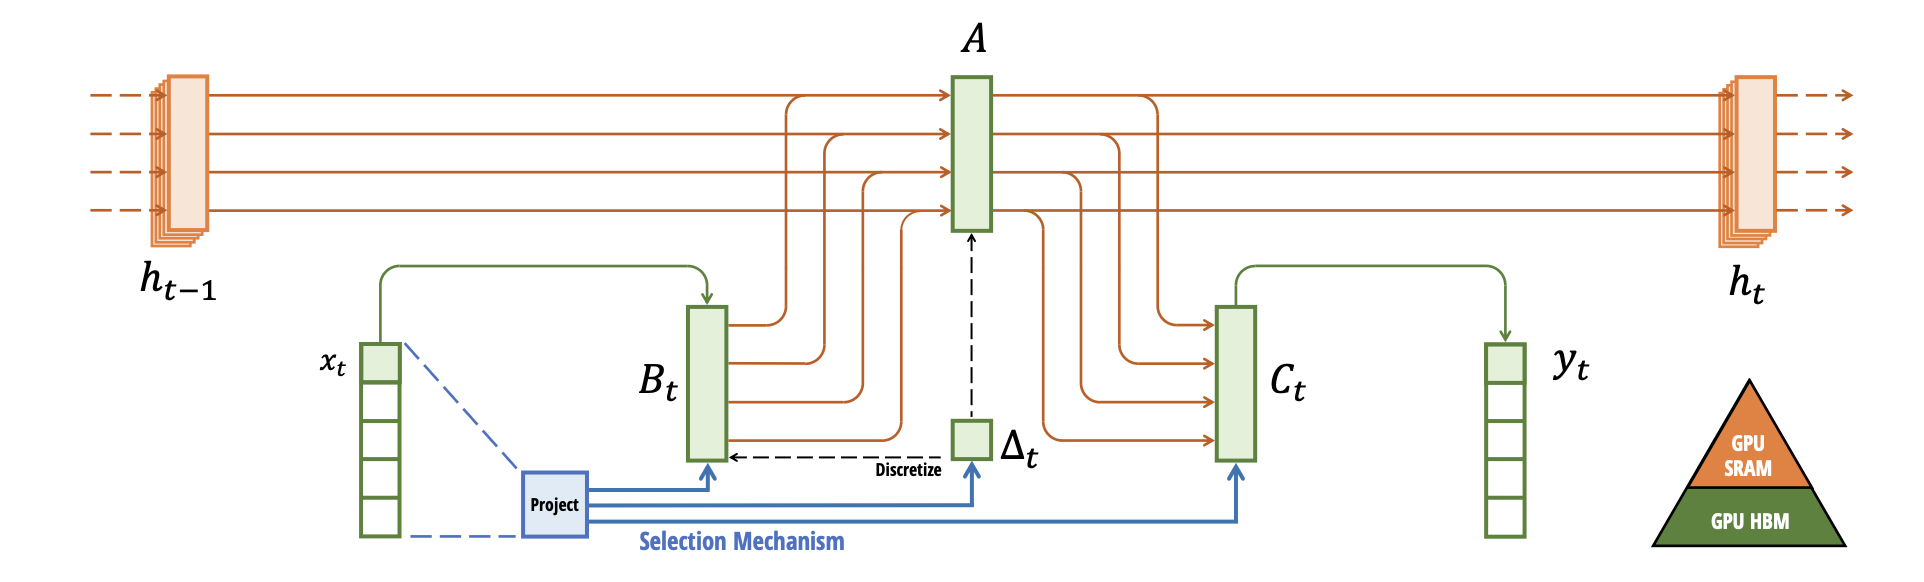
\includegraphics[width=0.85\textwidth]{images/fig_mamba_architecture.png}
    \caption[The Mamba block]{The Mamba block. Its parameters $\Delta_t$, $B_t$ and $C_t$ depend on the input $x_t$, so the model chooses
        what to remember, at a cost that grows only linearly with sequence length. Adapted from
        \cite{gu2023mamba}.}
    \label{fig:mamba_arch}
\end{figure}

The extension of SSMs to vision tasks has proceeded rapidly. Vision Mamba (Vim) \cite{zhu2024vision} proposed a vision backbone employing bidirectional Mamba blocks with position embeddings, achieving 2.8× faster inference than the DeiT transformer on ImageNet while using 86.8\% less GPU memory for high-resolution image processing. VMamba \cite{liu2024vmamba} introduced Visual State-Space (VSS) blocks with a 2D Selective Scan (SS2D) module that traverses image patches along multiple scan paths to capture two-dimensional spatial relationships. PlainMamba \cite{yang2024plainmamba} further explored non-hierarchical Mamba structures for visual recognition. These vision SSMs show that the linear cost of state space models can be used for visual tasks without losing accuracy.

The computational advantages of SSMs are particularly relevant for micro UAV applications. The O(n) complexity of SSMs, compared to the O(n²) complexity of transformers, directly translates to reduced inference time and memory consumption. The continuous-time formulation of SSMs also allows deployment at variable time scales without retraining, a property that Zubi\'{c} et al.~\cite{zubic2024state} report to be advantageous for event camera data, where the effective data rate varies with scene dynamics. Somvanshi et al.~\cite{somvanshi2025from} survey the development from S4 to Mamba and its variants, documenting the expanding application of SSMs across vision, language, and multi-modal tasks.

\section{State Space Models for Event Camera Data}
SSMs have only recently been applied to event-based vision. Zubi\'{c} et al.~\cite{zubic2024state} presented the first systematic investigation of SSMs for event camera data, published at CVPR 2024. They report a limitation of existing deep learning approaches to event data. When trained at one temporal resolution (i.e., a specific ratio between the number of events and the number of forward passes of the network), models based on CNNs, RNNs, and transformers all lose much of their accuracy when deployed at different temporal resolutions. This is particularly problematic for event cameras, where the event rate naturally varies with scene dynamics.

Zubi\'{c} et al.~\cite{zubic2024state} argued that SSMs, viewed as linear time-invariant (LTI) continuous-time systems, can be discretised at arbitrary step sizes without retraining. By rescaling a learnable timescale parameter by the ratio between training and inference frequencies, they report that their SSM-based models maintained performance across a range of deployment frequencies with minimal degradation (an average drop of 3.76 mAP over all test frequencies on Gen1 and 1Mpx, against more than 20 mAP for RNN and transformer detectors). They also report 33\% faster training than equivalent recurrent models. If these results hold, SSMs are architecturally well suited to the temporal characteristics of event camera data. Section~\ref{subsec:f2} tests the reported compensation under the released checkpoint and code, and Section~\ref{sec:robustness} tests a ConvLSTM detector in the same way.

The most influential baseline for event-based object detection is the Recurrent Vision Transformer (RVT) introduced by Gehrig and Scaramuzza \cite{gehrig2023recurrent}. RVT employs a four-stage hierarchical backbone combining convolutional priors with local and dilated global self-attention, using a ConvLSTM to carry hidden state across consecutive 50~ms windows \cite{gehrig2023recurrent}. A Feature Pyramid Network (FPN) and YOLOX detection head complete the pipeline \cite{gehrig2023recurrent}.

RVT achieved $47.2$~mAP on the Gen1 automotive dataset with an inference latency below 12~ms, a five-fold reduction compared to prior art \cite{gehrig2023recurrent}. All subsequent SSM-based methods, including those explored in this thesis, benchmark against RVT, making it the de facto reference architecture \cite{gehrig2023recurrent, zubic2024state, yang2025smamba}.

Zubi\'{c} et al.~\cite{zubic2024state}, described above, apply SSMs directly within the RVT framework for event-based object detection, achieving 47.71 mAP on Gen1 with S5 layers replacing the ConvLSTM. The SSM is used only to combine information across frames, while spatial feature extraction remains handled by Transformer attention blocks. The SSM variant employed is S5, a fixed-parameter (non-selective) model whose transition matrices do not depend on the input.

Most recently, SMamba \cite{yang2025smamba} (AAAI 2025) advances the state of the art on Gen1 to 50.4 mAP by replacing the spatial Transformer stages of RVT with a Sparse Selective Mamba (S6) backbone. A Spatio-Temporal Continuity Assessment (STCA) module identifies informative tokens and discards noisy or inactive patches before the Mamba scan. This reduces FLOPs by 23\% while improving accuracy. Inter-frame temporal context is provided by a ConvLSTM. SMamba thus shows that a selective Mamba can replace attention for spatial feature extraction in event-based detection while reducing computation.

The best-performing methods share a pattern. Each keeps inter-frame recurrence (an LSTM or SSM state carried across consecutive windows) and multi-scale FPN detection, and each changes several components of the RVT backbone at once. No prior work has compared a convolutional and a state-space spatial mixer under an otherwise identical backbone, temporal model and training pipeline. That controlled comparison, with a selective (Mamba) temporal recurrence in both models, is the primary architectural contribution of this thesis. The application of SSM-based event detection to micro-UAV platforms with SWaP constraints has no prior demonstration either, and remains outside the evaluation of this thesis (Section~\ref{sec:scope}).

\section[Event-Based Vision for UAV Navigation and Obstacle Avoidance]{Event-Based Vision for UAV Navigation\\ and Obstacle Avoidance}
Event cameras have been applied to UAV navigation because they suit high-speed, low-latency perception. Early work on event-based visual-inertial odometry by Rebecq et al.~\cite{rebecq2017real} showed that event cameras can estimate the camera's own motion accurately, which UAV localisation requires. Their approach tracked features in motion-compensated event frames and fused them with inertial measurements in a keyframe-based nonlinear optimisation to estimate the 6-DOF pose, remaining robust under rapid motion and high dynamic range.

Vidal et al.~\cite{vidal2018ultimate} extended this work by fusing events, standard frames and inertial measurements in a single state-estimation pipeline (Ultimate SLAM). The fusion improved accuracy by 130\,\% over an events-only and by 85\,\% over a frames-only visual-inertial pipeline, and remained reliable in high-speed and high-dynamic-range scenes, including on a flying quadrotor.

Falanga et al.~\cite{falanga2020dynamic} demonstrated event-based obstacle avoidance on quadrotors, building on their analysis of how perception latency limits the safe speed of a sense-and-avoid system \cite{falanga2019fast}. Their approach performed motion segmentation on the event stream to identify independently moving objects, then computed time-to-contact estimates to trigger avoidance manoeuvres. The system achieved an overall processing latency of approximately 3.5 milliseconds, enabling the quadrotor to avoid obstacles at relative speeds up to 10 m/s. Their work showed that event cameras allow reactive obstacle avoidance at speeds far beyond the capabilities of frame-based perception systems, where the minimum achievable latency is bounded by the frame period (about 17--33~ms at 30--60 frames per second).

Sanket et al.~\cite{sanket2020evdodgenet} proposed EVDodge, an event-based dodging system tested on UAV platforms. Their approach demonstrated real-time obstacle avoidance using purely event-based perception, showing that the high temporal resolution of event cameras could be directly translated into improved avoidance performance. The system was validated both in simulation and on physical quadrotor platforms, confirming the practical feasibility of event-based avoidance systems.

More recent work has explored bio-inspired processing pipelines for event-based UAV obstacle avoidance. Xu et al.~\cite{li2024taming} proposed BioDrone, which processes stereo event cameras with a chiasm-inspired pipeline for fast event filtering and obstacle detection and a lateral-geniculate-nucleus-inspired matching algorithm for obstacle localisation, deployed on an FPGA through software--hardware co-design, and reported an obstacle detection rate of 96.1\%. Such co-designed pipelines are particularly relevant for micro UAVs, where the power budget is a primary constraint.

Each of the surveyed approaches has limitations. The visual odometry and motion segmentation methods of Rebecq et al.\ \cite{rebecq2017real} and Falanga et al.\ \cite{falanga2020dynamic} use handcrafted features and geometric rules, which limits how well they generalise to new environments. EVDodge \cite{sanket2020evdodgenet}, while shown to work on real hardware, uses a relatively shallow network that has not been tested under challenging conditions such as cluttered scenes or rapidly changing lighting. The bio-inspired pipeline of Xu et al.\ \cite{li2024taming} is attractive for its low latency, but relies on a co-designed FPGA implementation and hand-designed filtering and matching stages rather than the learned spatial features required for general object detection. None of them combines learned deep spatial features with a temporal model that can handle variable event rates, the core gap that this thesis addresses through its SSM-based detection architecture.

\section{Event Camera Datasets and Benchmarks}
The DSEC dataset \cite{gehrig2021dsec}, developed at the University of Zurich, provides high-resolution stereo event camera data captured using Prophesee Gen3.1 sensors with a 60 cm baseline, complemented by global shutter colour cameras and LiDAR ground truth. DSEC covers a range of driving scenarios under both favourable and challenging illumination conditions, making it a valuable benchmark for event-based depth estimation and optical flow.

The MVSEC (Multi Vehicle Stereo Event Camera) dataset \cite{zhu2018multivehicle} uses DAVIS346B stereo pairs with a 10 cm baseline, providing synchronised event, frame, IMU, and LiDAR data. MVSEC includes sequences from indoor flying, outdoor driving, and motorcycle scenarios, offering diverse conditions for evaluating perception algorithms.

For object detection specifically, the Gen1 \cite{detournemire2020large} and 1Mpx \cite{perot2020learning} datasets provide large-scale automotive event recordings from Prophesee cameras with bounding-box annotations for cars and pedestrians in Gen1, and for pedestrians, two-wheelers and cars in 1Mpx.

Few datasets exist for UAV-specific scenarios. Most event camera datasets target automotive applications, and there are limited publicly available datasets that capture the specific challenges of micro UAV navigation, such as rapid ego-motion, indoor environments, small obstacles, and the particular motion patterns characteristic of rotary-wing flight. For the purposes of this thesis, the primary evaluation is conducted on the Gen1 automotive dataset, which provides a well-established benchmark for detection performance.

\section{Computational Constraints and Obstacle Avoidance for Micro UAVs}
Micro UAVs in the sub-250 gram class face severe SWaP constraints that shape the design of onboard perception systems. Typical computational platforms for nano- and micro-UAVs are milliwatt-class microcontrollers and parallel ultra-low-power processors, on which even a compact navigation network runs at only about 9--13 frames per second \cite{niculescu2021improving}. These platforms are orders of magnitude less capable than the GPU-equipped systems used to train and evaluate most deep learning models. This gap between training and deployment hardware requires either very efficient models, hardware acceleration, or offloading computation to a ground station at the cost of communication latency.

Several approaches to obstacle avoidance on resource-constrained platforms have been explored. Traditional methods based on optical flow divergence, time-to-contact estimation or event-based motion segmentation provide computationally lightweight avoidance capabilities but lack the ability to classify specific obstacles \cite{falanga2020dynamic, decroon2016monocular}. Model predictive control (MPC) approaches can generate optimal avoidance trajectories but require real-time environmental perception as input. Cooperative approaches, where a less-equipped micro UAV receives guidance from a sensor-rich companion \cite{pritzl2024drones}, offer a pragmatic solution but introduce communication dependencies.

The emergence of neuromorphic processing hardware offers a potential path to efficient onboard perception. The SynSense Speck chip \cite{synsense2026speck} integrates a dynamic vision sensor with a fully asynchronous spiking neural network processor, achieving real-time event processing with idle power consumption below 1 mW. Similarly, Intel's Loihi processors support on-chip learning and efficient SNN inference \cite{davies2021advancing}, and Loihi~2 adds programmable neuron models and graded spikes \cite{orchard2021efficient}. These platforms are particularly well-suited to processing event camera data, as they natively handle the sparse, asynchronous data format. However, the software ecosystem for neuromorphic processors remains immature compared to conventional deep learning frameworks, and mapping complex detection architectures onto neuromorphic hardware is still an open problem.

Their linear cost makes SSM-based architectures candidates for deployment on the limited computational resources available on micro UAVs. Unlike transformer-based models, whose memory and computation grow quadratically with sequence length, SSMs process long event sequences with a fixed-size recurrent state, although that state can be large (Section~\ref{sec:efficiency}). Combined with model compression techniques such as quantisation and pruning, SSM architectures may enable real-time object detection on platforms that cannot support transformer or large CNN inference.

\section{Spiking Neural Networks for Event-Based Detection}
\label{sec:snn_detection}
Directly trained spiking neural networks (SNNs) are an established family on this benchmark and the
comparison class for the neuromorphic strand of this thesis. They are trained with surrogate
gradients~\cite{neftci2019surrogate}. The non-differentiable spike function is kept in the forward pass
and replaced by a smooth surrogate derivative in the backward pass, which makes back-propagation through
time applicable to networks of spiking neurons. Table~\ref{tab:snn_landscape} places the spiking detectors
reported on Gen1 against the non-spiking models of this thesis.

\begin{table}[htbp]
\centering
\small
\caption[Spiking and non-spiking detectors on Gen1]{Published detectors on the Gen1 test set (mAP). Ranges cover different model sizes. $T\times D$: time steps
    $\times$ sub-steps of a spiking model ($D=1$: plain binary spikes).}
\label{tab:snn_landscape}
\begin{tabularx}{\textwidth}{@{}l>{\raggedright\arraybackslash}Xccl@{}}
\toprule
\textbf{Model} & \textbf{Type} & \textbf{$T\times D$} & \textbf{mAP} & \textbf{Venue} \\
\midrule
RVT \cite{gehrig2023recurrent}        & ANN (attention, ConvLSTM) & --- & 47.2 & CVPR 2023 \\
S5-RVT \cite{zubic2024state}          & ANN (attention, S5)       & --- & 47.7 & CVPR 2024 \\
SMamba \cite{yang2025smamba}          & ANN (sparse Mamba, ConvLSTM) & --- & 50.4 & AAAI 2025 \\
EventSSM (this thesis)                  & ANN (convolution, Mamba-2) & --- & 46.2 & --- \\
PureSSM (this thesis)                   & ANN (BiMamba, Mamba-2)    & --- & 46.4 & --- \\
\midrule
HsVT \cite{xu2025hybrid}              & hybrid (spiking temporal block) & --- & 44.9--47.8 & ICML 2025 \\
SpikeDet \cite{fan2025spikedet}       & SNN, integer-valued       & $5\times1$, $4\times2$ & 46.5--47.6 & preprint \\
EAS-SNN \cite{wang2024eas}            & SNN, recurrent            & $3$ & 37.2--40.9 & ECCV 2024 \\
SpikeYOLO \cite{luo2024integer}       & SNN, integer-valued       & $5\times1$, $4\times2$ & 38.5--40.4 & ECCV 2024 \\
EMS-YOLO \cite{su2023deep}            & SNN                       & $5$ & 26.7--31.0 & ICCV 2023 \\
\bottomrule
\end{tabularx}
\end{table}

The accuracy gap between spiking and non-spiking detectors on Gen1 has
closed. EMS-YOLO, the first deep directly trained spiking detector~\cite{su2023deep}, reached 31.0 in 2023,
16.7~mAP below S5-RVT. The strongest recent spiking detectors, SpikeDet~\cite{fan2025spikedet} and
HsVT~\cite{xu2025hybrid}, report 47.6 and 47.8, level with S5-RVT and above this thesis models.
On this benchmark a spiking detector is therefore no longer necessarily a less accurate one, and the case
for the neuromorphic strand rests on energy and deployment rather than accuracy.

The mechanisms behind that progress are identifiable, and both are native to a state-space neuron. The first is more information per spike. SpikeYOLO's I-LIF neuron emits integer values in $\{0,\dots,D\}$ during
training and, at inference, expands each integer into $D$ binary spikes over virtual timesteps, so that
inference remains spike-driven (binary, accumulate-only) while training sees a multi-bit
signal~\cite{luo2024integer}. SpikeDet uses the same integer-valued scheme, and for both detectors the
$4\times2$ configuration, with fewer timesteps each carrying a two-level value, outperforms $5\times1$. The second is temporal state. EAS-SNN uses recurrent convolutional SNNs with temporal memory as an adaptive event sampler~\cite{wang2024eas},
and HsVT combines LSTM blocks with a spiking temporal feature-extraction block on a MaxViT spatial
backbone~\cite{xu2025hybrid}. HsVT is the closest design point to the spiking model of this thesis. It keeps
spatial processing in non-spiking form and spikes along time. A state-space neuron supplies both mechanisms
by construction, since its state is a carried, multi-valued memory and the graded readout of
Section~\ref{subsec:readout_modes} is the per-neuron analogue of an integer-valued spike. EMS-YOLO and
SpikeYOLO also report an ANN of equivalent architecture, so the overall cost of spiking is known for those designs, but where that cost comes from is not reported.

\section{Spiking State Space Models}
\label{sec:spiking_ssm}
A discretised diagonal state space model and a leaky integrate-and-fire neuron are the same linear
recurrence with different readouts. Consider one state dimension of a diagonal SSM with decay $a<0$,
input weight $b$, output weight $c$ and step $\Delta$, discretised with a zero-order hold:
\begin{equation}
  h_t = \bar a\, h_{t-1} + \bar b\, u_t, \qquad y_t = c\, h_t, \qquad
  \bar a = e^{\Delta a}, \quad \bar b = \frac{e^{\Delta a}-1}{a}\, b .
  \label{eq:ssm_scalar}
\end{equation}
The discrete LIF neuron of Equations~\eqref{eq:lif_integrate}--\eqref{eq:lif_reset} integrates its input
$x_t$ as $m_t = \beta m_{t-1} + x_t$. With $\beta = \bar a$ and $x_t = \bar b u_t$ the membrane potential
$m_t$ is exactly the SSM state $h_t$, and the leak is a discretised decay. This match needs three conditions. The decay $a$ must be a single real number, the step $\Delta$ must stay fixed, and the input must be held constant during each step. S4D and S5 usually use complex decays, which make the state oscillate, and a LIF neuron cannot do
that. In Mamba the step changes with the input, so the matching leak would change at every step. The neuron differs in two
respects only. Its readout is a threshold, $s_t = \Theta(m_t - \vartheta)$, instead of a linear map. Its
reset, $m_t \leftarrow m_t - s_t\vartheta$, feeds the output back into the state. Without reset the recurrence is linear and can be evaluated with a parallel scan, as
SSMs are during training. With reset, the state depends on its own thresholded past, and the recurrence must
be unrolled sequentially. Much of the spiking-SSM literature consists of ways around that obstacle,
summarised in Table~\ref{tab:spiking_ssm}.

\begin{table}[htbp]
\centering
\small
\caption[Spiking state space models]{Spiking state space models in the literature. All but the last were built for one-dimensional sequences, not
    images.}
\label{tab:spiking_ssm}
\begin{tabularx}{\textwidth}{@{}l>{\raggedright\arraybackslash}X>{\raggedright\arraybackslash}Xl@{}}
\toprule
\textbf{Work} & \textbf{How spiking enters} & \textbf{Parallel training} & \textbf{Task} \\
\midrule
SpikingSSMs \cite{shen2025spikingssms} & spiking neurons with learnable thresholds driven by an S4D-type SSM &
  a small network predicts the after-reset membrane & LRA, WikiText-103 \\
SPikE-SSM \cite{zhong2024spike} & reset-refractory neuron, trainable thresholds & boundary compression of
  the membrane & LRA, WikiText-103 \\
P-SpikeSSM \cite{bal2025p} & spikes sampled stochastically from an SSM-based neuron & sampling replaces
  sequential spike generation & long-range tasks \\
SiLIF \cite{fabre2025silif} & the neuron is a two-state SSM with S4-style parameterisation & --- (surrogate
  gradients through time) & speech \\
Spiking-S4 \cite{du2023spiking} & spiking neurons combined with an S4 model & --- & speech enhancement \\
SpikeMba \cite{li2024spikemba} & spiking saliency detector for proposals; Mamba non-spiking & --- &
  video grounding \\
\midrule
This thesis & LIF readout on the output of a selective (Mamba-2) temporal block & SSM scan unchanged;
  readout unrolled over the clip & event detection \\
\bottomrule
\end{tabularx}
\end{table}

SpikingSSMs~\cite{shen2025spikingssms} train a lightweight surrogate network to predict the
after-reset membrane potential, which restores parallel training with speed-ups over
iterative unrolling, and report performance competitive with non-spiking SSMs at about 90\,\% network
sparsity. SPikE-SSM~\cite{zhong2024spike} accelerates the same computation by compressing the membrane
dynamics between spike boundaries and adds a reset-refractory neuron with trainable thresholds.
P-SpikeSSM~\cite{bal2025p} avoids sequential spike generation altogether by sampling spikes stochastically
from an SSM-based neuronal model. SiLIF~\cite{fabre2025silif} takes the correspondence of
Equation~\eqref{eq:ssm_scalar} in the other direction. It makes it exact for a two-state adaptive neuron and
gives the neuron an S4-style parameterisation (decays trained in logarithmic form, a learnable per-neuron step,
and a complex-valued variant with oscillatory dynamics), reporting the best accuracy among spiking neuron models on speech. Spiking-S4~\cite{du2023spiking} combines S4 with spiking neurons for speech
enhancement at reduced parameter and FLOP counts.

Spiking models target one-dimensional sequence tasks such as long-range benchmarks, language modelling and speech. It is also built on linear time-invariant SSMs (S4, S4D), whose
decay does not depend on the input. The only selective model in Table~\ref{tab:spiking_ssm}, SpikeMba, keeps
Mamba itself non-spiking and uses spikes only for proposal generation~\cite{li2024spikemba}. In a selective
SSM the decay $\bar a_t = e^{\Delta_t a}$ varies with the input at every step. The recurrence is still linear
in the state, so a spiking readout placed after the scan, as in this thesis, leaves the scan exact and parallel. Making the selective state itself spike, with a reset inside the scan, would require one of the
parallel-training devices above to be extended to input-dependent decays.

\section{Neuromorphic Hardware and the Deployment Path}
\label{sec:neuromorphic_hw}
Neuromorphic processors execute spiking networks in an event-driven manner. Computation and communication happen only when spikes arrive, so energy scales with activity rather than with the size of
the input~\cite{davies2021advancing}. Two features of Intel's Loihi~2 matter for state space models.
Its neuron models are programmable in microcode, so any small
per-neuron recurrence, including the state update of a diagonal SSM, can be implemented directly. It also
supports graded spikes, which carry an integer payload rather than a single bit~\cite{orchard2021efficient},
the hardware counterpart of integer-valued and graded readouts.

Meyer et al.~\cite{meyer2024diagonal} gave the first implementation of an SSM on neuromorphic hardware,
mapping S4D to Loihi~2. The comparison with an NVIDIA Jetson Orin Nano depends on the processing mode. In
offline, batched, sample-by-sample processing the Jetson performed better. In token-by-token processing,
Loihi~2 consumed about 1000 times less energy, with 75 times lower latency and 75 times higher throughput,
than a recurrent S4D implementation on the Jetson. Token-by-token processing is exactly the regime of a
streaming event camera, which is why this result motivates the neuromorphic strand. It was obtained for a
linear time-invariant SSM on one-dimensional sequence benchmarks. A selective SSM, whose decay must be
recomputed from the input at every step, and a two-dimensional detection backbone remain untested on such
hardware. Other neuromorphic substrates take a different route. SynSense's Speck integrates an event sensor
and a spiking processor on one chip~\cite{synsense2026speck}.

Energy figures for spiking detectors run on GPUs are estimates. The convention in the
detection literature is to count synaptic operations and multiply them by a per-operation energy, typically
0.9~pJ for a 32-bit floating-point accumulate against 4.6~pJ for a multiply--accumulate at
45~nm~\cite{luo2024integer,su2023deep,horowitz2014computing}. Such estimates ignore memory access and data
movement, which dominate energy on real hardware, so they rank designs rather than predict silicon consumption. Measured results such as Meyer et al.'s are rare by comparison.

The software path is in transition. Intel archived its Lava framework on 13 May 2026, stated that it will
no longer maintain it, and announced a successor SDK without a public timeline~\cite{intel2026lava}. The
Neuromorphic Intermediate Representation (NIR) defines a common set of computational primitives through
which models can be exchanged between simulators and neuromorphic hardware~\cite{pedersen2024neuromorphic},
and is the export format chosen in this thesis for that reason (Section~\ref{sec:neuro_case}).

\section{Research Gaps}
\label{sec:gaps_revisited}
\label{sec:gaps_thesisA}% old label of the Thesis-A gap list, kept so that any old reference still resolves
Thesis~A identified four gaps, all framed around an integrated detection-and-avoidance system for micro-UAVs.
The scope change of Section~\ref{sec:scope_change} altered each of them. Gap~1 asked for a selective Mamba
detector free of both recurrence and convolution, compared with a CNN--SSM hybrid under one pipeline. The
models built here carry a Mamba state from one window to the next and keep a strided convolutional stem, so
only the controlled comparison survives, as Gap~A below. Gap~2, a detector joined to an avoidance controller
on a micro-UAV, was retired together with the integration aim. Gap~3 noted that the latency, memory and
energy of SSM detectors had not been measured on drone hardware. Section~\ref{sec:efficiency} measures all
three for every model, but on a desktop GPU, so this gap is answered only in part. Gap~4 assumed that SSMs
generalise across event rates better than other detectors~\cite{zubic2024state}. It became a test of that
claim, Gap~B below. The three gaps that remain are narrower than the originals, and each is answered in one
part of Chapter~\ref{ch:results}.

Gap~A is the isolated effect of the spatial mixer. Published SSM detectors change several components
at once. S5-RVT replaces the temporal mixer of an attention backbone with S5~\cite{zubic2024state}. SMamba
replaces the spatial attention with a sparse Mamba, adds token selection and keeps a ConvLSTM in time,
reaching 50.4~mAP on Gen1~\cite{yang2025smamba}. Neither result shows what the spatial mixer contributes on
its own, because no published detector compares a convolutional and a state space mixer with the temporal
model, neck, head and training recipe held fixed. Section~\ref{sec:acc_results} makes that comparison with
EventSSM and PureSSM, and Section~\ref{sec:erf} measures how much of the image each mixer draws on.

Gap~B is rate robustness under the published artefacts. Zubi\'{c} et al.~\cite{zubic2024state}
report that an S5 detector keeps 39.84 of its 47.7~mAP at ten times the training rate once its step
$\Delta$ is rescaled, while RVT's ConvLSTM falls to 8.35~mAP. These two numbers are the published evidence
that SSMs, unlike recurrent networks, cope with changes in the event rate. The released code cannot produce
test data at a faster frame rate, because its 50-ms step is fixed, so neither number had been checked with
frames that really arrive faster. Section~\ref{sec:robustness} builds such data and tests both claims with
the released checkpoints.

Gap~C is where the cost of spiking comes from. Spiking detectors now match non-spiking ones on Gen1. SpikeDet reports 46.5 to 47.6~mAP and HsVT 44.9 to 47.8 (Table~\ref{tab:snn_landscape}). Spiking SSMs exist
for sequence tasks (Table~\ref{tab:spiking_ssm}), but, to the author's knowledge, none combines a selective
temporal core with spiking for event-based detection. The surveyed detectors report at most one difference
between a spiking model and a non-spiking one. None splits it into the cost of the neuron dynamics, of
sparsity and of binarisation, against a non-spiking twin trained through the same pipeline. The three
readouts of Section~\ref{subsec:readout_modes} share one membrane and are built to measure that split
(Section~\ref{sec:spiking_results}).

% ===================================================================== CHAPTERS 3-7 (skeleton: write here)

\chapter{Methodology}
\label{ch:method}

\section{Event Representation}
\label{sec:repr}
Every model takes stacked-histogram as inputs~\cite{gehrig2023recurrent}. The
asynchronous event stream is cut into consecutive 50-ms windows that do not overlap, and within each window the events are counted per
pixel, separately for each polarity and for each of ten equal time bins. This gives $2 \times 10 = 20$
channels at the sensor's resolution, $(20, 240, 304)$
(Equations~\eqref{eq:sh_bin}--\eqref{eq:sh_count}, Appendix~\ref{app:maths}). Each count is capped at 10,
and the pipeline zero-pads the tensor to $(20, 256, 320)$. The feature maps passed to the detection neck
are then $32\times40$, $16\times20$ and $8\times10$ at strides 8, 16 and 32. The representation is sparse. On average, only 1.5\,\% of its entries are non-zero (between 0.2 and 4.0\,\% per recording, depending on
scene activity), and the cap is reached by only about 0.2\,\% of the non-zero entries.

This representation was chosen to keep the architectural study controlled. Stacked histograms are the
input of the S5-RVT baseline, which was reproduced in Thesis~A, and keeping the same representation is
essential for a fair comparison between the backbones of the baseline and the new models. Alternative
representations are reviewed in Chapter~\ref{ch:lit}. The detector
makes one prediction every 50~ms, or 20 times per second, and its response can never be faster than one
window (Section~\ref{sec:latency_window}).
\section{The Frozen Detection Pipeline}
\label{sec:frozen_pipeline}
A key design choice of this thesis is that the detection pipeline around the backbone never changes. Every
model reuses the same S5-RVT pipeline. The data loading, the neck, the detection head, the loss, the
evaluation and the training loop are all frozen and kept the same for every model. Through a configuration
setting and a short registration step, the baseline's backbone can be replaced with a new one, while the
original baseline code stays unedited. Figure~\ref{fig:spiking_arch}(a) shows the shared pipeline. Because
nothing else in the pipeline changes, any difference in results can only come from the backbone. EventSSM
and PureSSM differ only in their spatial mixer, so a difference between them can be traced back to that
single component. The comparison between the baseline and the new models is less strict than the
comparison between the new models themselves. Both of the baseline's mixers differ from those of the new
models, and the new models were trained with a batch size of 4 instead of 8, to fit the memory of the local
GPU, and with a lower numerical precision (Section~\ref{sec:training}).

\begin{figure}[htbp]
    \centering
    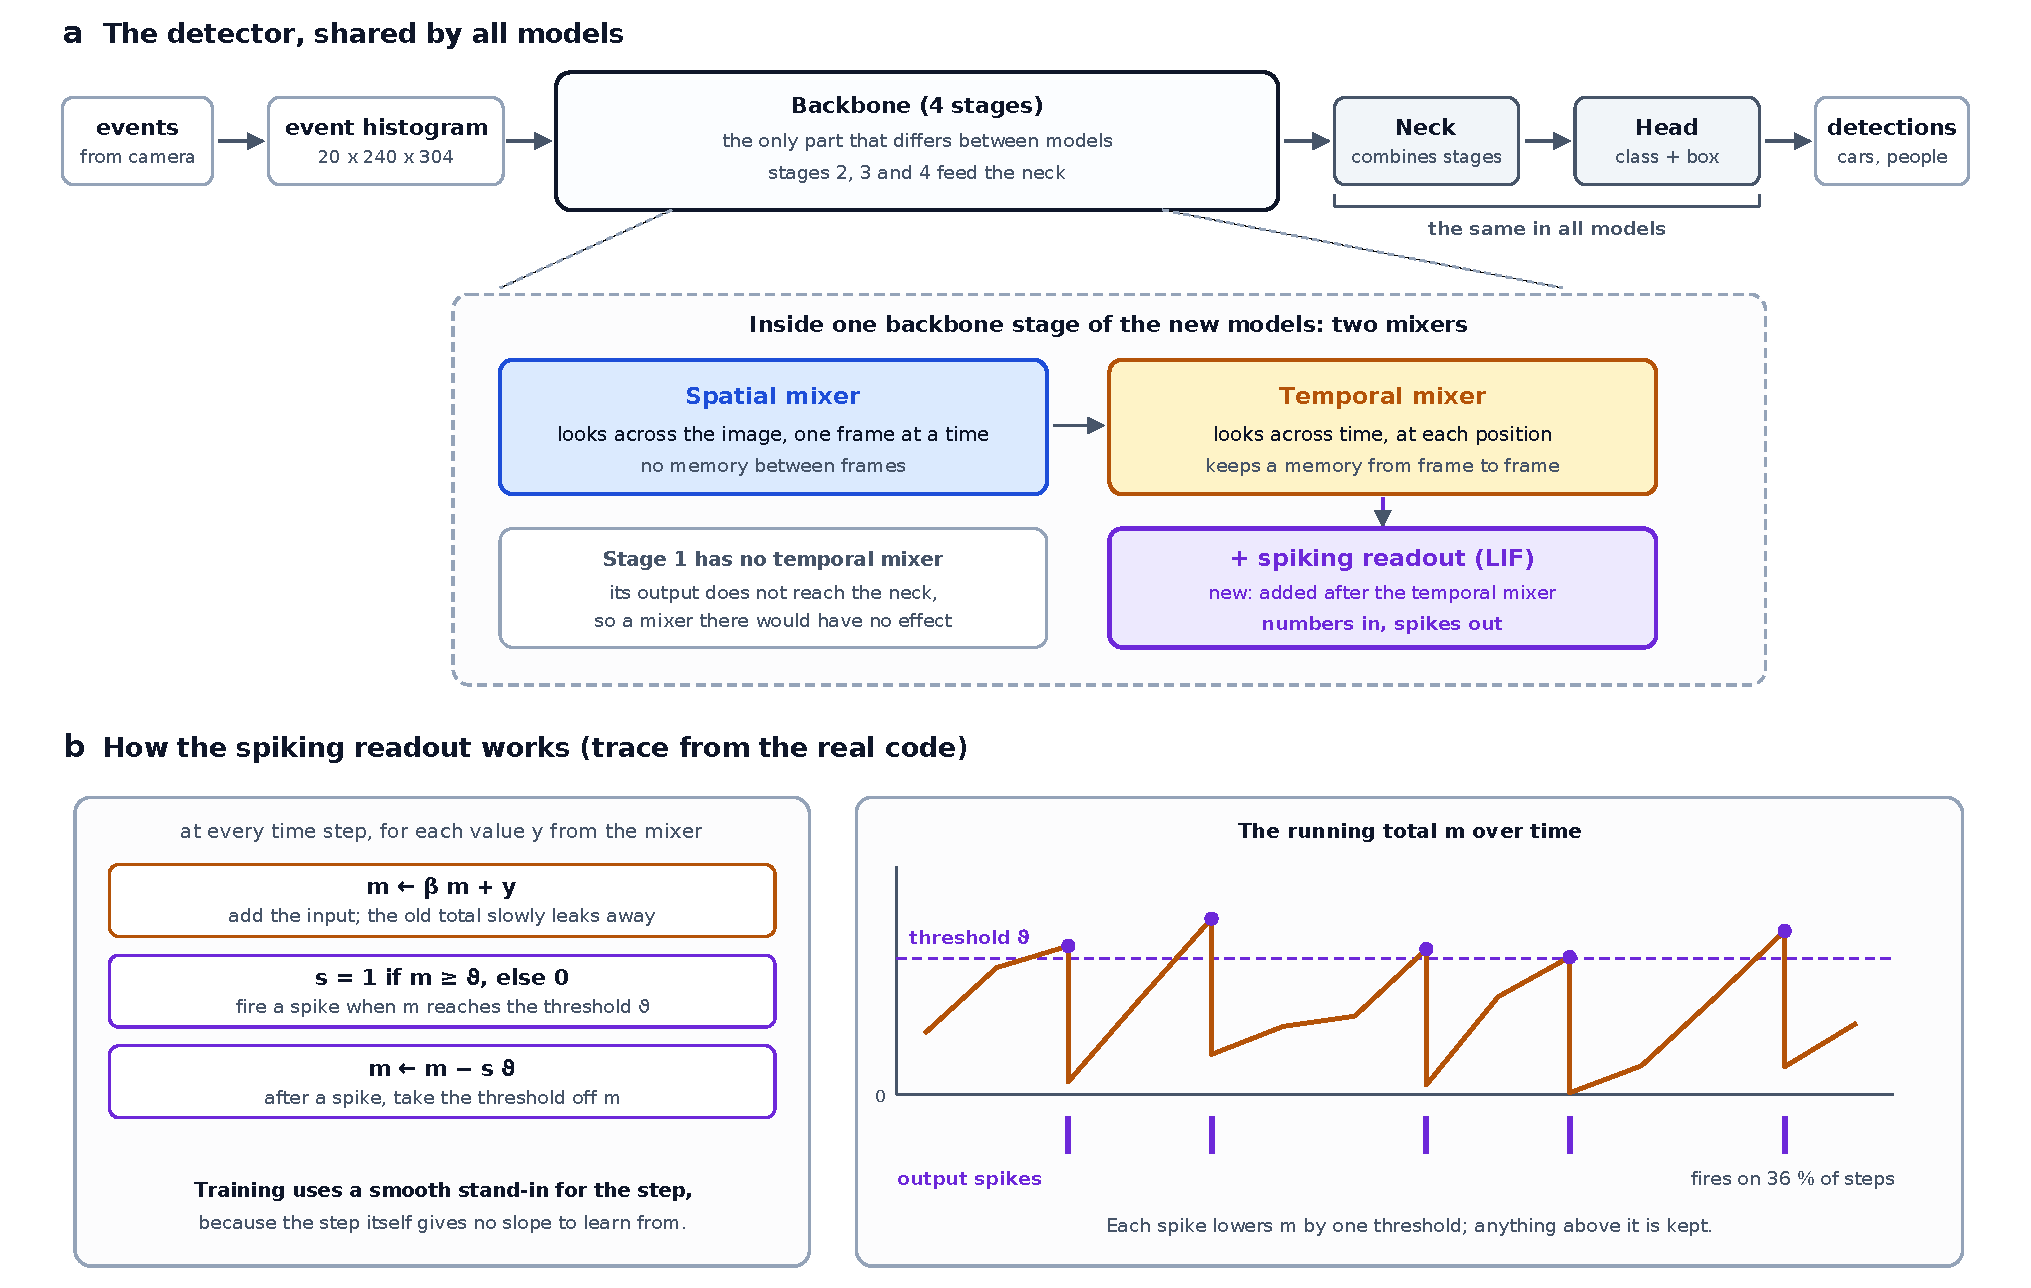
\includegraphics[width=\textwidth]{images/fig_spiking_architecture_compact.pdf}
    \caption[The detector and the spiking readout]{The detector. (a) The pipeline shared by all models; only the
        backbone differs (Table~\ref{tab:four_models}). (b) The spiking (LIF) readout.}
    \label{fig:spiking_arch}
\end{figure}

\subsection{Neck, Head and Loss}
\label{subsec:neck_head}
The neck combines the feature maps from backbone stages 2, 3 and 4. It passes information back and forth
between the coarse and the fine maps, so that every output combines precise location with wider context.
YOLOX is used as the detection head~\cite{ge2021yolox}. At every cell of each feature map, it predicts how
likely it is that an object is present, which class the object belongs to, and where its box lies. During
training, a matching rule called SimOTA decides which cells are responsible for which object. The training
loss is the sum of three terms:
\begin{equation}
  \mathcal{L} \;=\; \mathcal{L}^{\mathrm{BCE}}_{\mathrm{obj}} + \mathcal{L}^{\mathrm{BCE}}_{\mathrm{cls}}
  + 5\,\big(1 - \mathrm{IoU}^2\big).
  \label{eq:loss}
\end{equation}
The first two terms measure the errors in the object and class predictions, while the third measures how
well the predicted box overlaps the true bounding box from the dataset. The third term is weighted five
times more strongly than the other two.

\subsection{The Two Mixing Axes}
\label{subsec:two_axes}
Each backbone stage mixes information along two axes. The spatial mixer sees the $H \times W$ positions of a
single frame, from $32 \times 40$ at stage~2 down to $8 \times 10$ at stage~4, and keeps no state between
frames. In EventSSM it is a ResNet-18 convolution, and in PureSSM a bidirectional Mamba (BiMamba) scan over
rows and columns (Table~\ref{tab:four_models}). The temporal mixer sees the other axis, the sequence of
frames at each of those positions, through one causal Mamba-2 layer per stage~\cite{dao2024transformers}. Its
state carries over from one 21-frame clip of a recording to the next, while gradients stop at every clip
boundary, a form of truncated backpropagation through time (TBPTT, Section~\ref{sec:training}). The same
Mamba-2 scan runs over a whole clip in training and one frame at a time at test time, so the state follows
the same equations in both.

Because the two mixers act on different axes, either can be replaced without touching the other. EventSSM
and PureSSM differ only on the spatial axis, and SpikingSSM only on the temporal one, where a leaky
integrate-and-fire (LIF) readout follows each Mamba-2 layer (Section~\ref{subsec:spiking_method}). Temporal
blocks sit only on stages 2, 3 and 4, the ones the neck reads, and each branches off its stage. Its output goes to the neck, while the next spatial stage continues from the per-frame features.
RVT~\cite{gehrig2023recurrent} instead passes each stage's recurrent output to the next stage. All the new
models use the branching design, so it does not bias the comparison between them. Keeping a state at every
position of three stages has a measurable cost. The Mamba models carry 144.5~MB of state per video stream,
31 times the 4.7~MB of RVT and S5-RVT (Section~\ref{sec:efficiency}).
\newpage
\section{Model Architectures}
\label{sec:models}
Table~\ref{tab:four_models} shows the models compared in this thesis. RVT, which uses a ConvLSTM temporal
mixer to process time, is the original baseline from the literature. S5-RVT replaces the ConvLSTM with an S5 state space layer. It was reproduced in Thesis~A as the minimum viable product. The first new model,
EventSSM, combines a convolutional spatial mixer with a Mamba-2 temporal mixer. PureSSM replaces the
convolutional mixer of EventSSM with a state space one. Finally, SpikingSSM adds a spiking output to
PureSSM's temporal mixer.

\begin{table}[htbp]
\centering
\caption[The five models compared]{The five models compared. Bold: the one part that changes from the row above. EventSSM differs from S5-RVT
    in both parts.}
\label{tab:four_models}
\begin{tabularx}{\textwidth}{@{}l>{\raggedright\arraybackslash}X>{\raggedright\arraybackslash}X>{\raggedright\arraybackslash}X@{}}
\toprule
\textbf{Model} & \textbf{Spatial mixer} & \textbf{Temporal mixer} & \textbf{Role} \\
\midrule
RVT & MaxViT (local + grid attention) & ConvLSTM & Literature baseline \\
S5-RVT & MaxViT & S5 (diagonal SSM) & Reproduced reference \\
EventSSM (this thesis) & ResNet-18 conv, 3$\to$20-ch adapted, ImageNet-init & Mamba-2 (causal, per-pixel) & CNN--SSM hybrid \\
PureSSM (this thesis) & \textbf{BiMamba} (bidirectional scan) & Mamba-2 (identical) & Pure state-space detector \\
SpikingSSM (this thesis) & BiMamba (identical) & Mamba-2 $+$ \textbf{LIF readout} & Spiking detector \\
\bottomrule
\end{tabularx}
\end{table}

\subsection{Baseline: S5-RVT}
\label{subsec:s5rvt}
S5-RVT~\cite{zubic2024state} is the RVT detector~\cite{gehrig2023recurrent} with its ConvLSTM replaced by
an S5 state space layer. It uses MaxViT attention~\cite{tu2022maxvit}, which first compares nearby patches
and only after that compares patches spread across the entire image. The model has 18.19 million
parameters. It serves as the reference for this thesis because it is the published state space event
detector on the Gen1 dataset with released code and trained weights. The weights used were exactly the
published ones, no retraining took place, and they reproduced the published result exactly
(Section~\ref{sec:repro_results}).

\subsection{EventSSM: Convolutional Spatial, State-Space Temporal}
\label{subsec:eventssm}
EventSSM uses ResNet-18~\cite{he2016deep} as its spatial mixer. ResNet-18 is a widely used convolutional
network, and it starts here from weights pre-trained on the ImageNet photo dataset. It is made up of a
first layer and a pooling step, which together shrink the image four times, followed by four stages. The
first stage keeps the size of the feature map and each later stage halves it. The first layer expects the
three colour channels of a photograph, whereas the input here has 20 channels. The first layer is therefore
adapted by averaging its weights over the three colour channels and copying the result to all 20 channels,
scaled so that the overall response stays the same:
\begin{equation}
  W'_{:,c} \;=\; \frac{3}{20}\cdot\frac{1}{3}\sum_{k=1}^{3} W_{:,k}, \qquad c = 1,\dots,20.
  \label{eq:avg_projection}
\end{equation}
Here $W$ is the original weight and $W'$ the adapted one. In this way, the edge and shape detectors learned
on photographs remain useful for all channels of the event input.

For the time axis, EventSSM uses one Mamba-2 layer~\cite{dao2024transformers} on each of stages 2, 3 and 4.
Each position is treated as its own sequence over time, so the layer follows how the features at that
position change from frame to frame. At every time step $t$, each part $j$ of the layer updates a memory $H$
and produces an output $y$:
\begin{align}
  H^{(j)}_t &= \exp\!\big(\Delta^{(j)}_t a^{(j)}\big)\, H^{(j)}_{t-1} + \Delta^{(j)}_t\, x^{(j)}_t B_t^{\top},
  \label{eq:mamba2_state}\\
  y^{(j)}_t &= H^{(j)}_t C_t + D^{(j)} x^{(j)}_t.
  \label{eq:mamba2_out}
\end{align}
In the first equation, the old memory is multiplied by a decay factor and the new input $x_t$ is added. The
decay depends on the learned rate $a<0$ and the step size $\Delta_t>0$. $B_t$ and $C_t$ are projections
that control how the input is written into the memory and read out of it, and $D$ passes part of the input
straight through to the output. The main feature of Mamba compared with S4 or S5 is that the step size
depends on the current input, which allows the model to decide, at every moment, how much of the memory to
keep. EventSSM has a total of 19.18 million parameters.

\subsection{PureSSM: State-Space Spatial and Temporal}
\label{subsec:puressm}
PureSSM replaces each convolutional stage of EventSSM with a stack of bidirectional Mamba blocks.
Apart from a small $3\times3$ filter inside each block, convolution is kept only where it shrinks the image, at the start of the network and between the stages.
The four stages contain 2, 2, 8 and 2 blocks, fourteen in total, and stochastic
depth~\cite{huang2016deep} is used during training as a regularisation method. Whereas EventSSM starts
from pre-trained weights, PureSSM was trained from scratch. It contains the fewest parameters, 16.33
million, which makes it the smallest model in this thesis.

Each block processes a feature map $X$ in two steps:
\begin{align}
  X' &= X + \mathrm{DWConv}_{3\times3}(X), \label{eq:bimamba_local}\\
  X_{\mathrm{out}} &= X' + \mathrm{DropPath}\big(\mathrm{BiScan}(\mathrm{LN}(X'))\big). \label{eq:bimamba_block}
\end{align}
The first step adds a $3\times3$ filter that starts at zero, so each block begins as a pure scan and then
learns during training how much local detail to add. The second step flattens the image into a sequence and
scans through it with Mamba. Here, $\mathrm{LN}$ is layer normalisation and $\mathrm{DropPath}$ is the stochastic
depth mentioned above. The image is read row by row in some blocks and column by column in
others~\cite{li2024mamband}, which allows information to spread in both directions across the image. Each
scan runs both forwards and backwards over the sequence, which is why the block is called
bidirectional~\cite{zhu2024vision}:
\begin{equation}
  \mathrm{BiScan}(u) \;=\; W_{\mathrm{out}}\,\mathrm{RMSNorm}\Big(\big[\,\overrightarrow{\mathrm{SSM}}(u)
  + \mathrm{flip}\big(\overleftarrow{\mathrm{SSM}}(\mathrm{flip}(u))\big)\big]\odot\mathrm{SiLU}(z)\Big),
  \label{eq:biscan}
\end{equation}
where $\mathrm{flip}$ reverses the order of the sequence and $z$ is a gate computed from the input. The
forward and backward scans each follow the update of Equation~\eqref{eq:mamba2_state} and are then added
together. This allows every position to draw on information from the whole image.

The whole frame is available at once, so looking in both directions is allowed within a frame. The spatial
scan starts fresh for each frame. This is a design choice, so that no information leaks from one frame to
the next. As in EventSSM, time is handled only by the temporal blocks. The comparison between the two
models therefore isolates the spatial mixer, together with the fact that EventSSM is pre-trained and
PureSSM is not.
\newpage
\subsection{SpikingSSM: A Spiking Temporal Readout}
\label{subsec:spiking_method}
The spiking variant keeps PureSSM's Mamba memory unchanged. Only the output of the memory passes through
spiking neurons of the leaky integrate-and-fire (LIF) type. At each time step $t$, each neuron updates its
potential $m_t$, decides whether to fire a spike $s_t$, and then resets:
\begin{align}
  m_t &= \beta\, m_{t-1} + y_t, \label{eq:lif_integrate}\\
  s_t &= \Theta(m_t - \vartheta), \label{eq:lif_fire}\\
  m_t &\leftarrow m_t - s_t\,\vartheta. \label{eq:lif_reset}
\end{align}
The potential leaks away at a rate set by $\beta$, while the new input $y_t$ is added. When the potential
reaches the threshold $\vartheta$, the neuron fires ($\Theta$ is the step function). The threshold is then
subtracted from the potential, so the excess carries over to the next step. The leak $\beta$ was started at
0.9 and learned separately for each channel, and a squeezed sigmoid keeps it between 0 and 1. The
threshold was fixed at 1 for every neuron and was not learned. Spiking neurons are used on all three
stages that feed the neck, and the model has 16.34 million parameters.

Spikes are events in time, which is why they were added along the time direction. The temporal block already steps through time, so no extra time steps are needed. A fully spiking detector, by contrast,
usually repeats each input four or five times (Table~\ref{tab:snn_landscape}). The spatial mixer looks in
both directions across the image and has no time axis, so it stays non-spiking, which makes this model a
hybrid.

Because a spike is only on or off and has no slope, training uses a smooth curve as a stand-in for the slope,
used only when the weights are updated:
\begin{equation}
  \frac{\partial s_t}{\partial m_t} \;\approx\; \frac{\alpha/2}{1 + \left(\tfrac{\pi}{2}\alpha (m_t-\vartheta)\right)^2},
  \label{eq:surrogate}
\end{equation}
with $\alpha = 2$. When the model runs, it still produces real on/off spikes.

\subsection{Readout Modes and the Readout Ladder}
\label{subsec:readout_modes}
The same neurons can pass on their activity in three ways. The spike readout passes its
information in binary, as 1 or 0. The graded readout sends a spike that also carries the value of
the potential, like the graded spikes of the Loihi~2 neuromorphic chip~\cite{orchard2021efficient}. The
analog readout sends the potential at every step, so its output is never zero. Together with PureSSM,
the three readouts form a ladder in which each step adds one spiking property:
\begin{equation}
\begin{aligned}
  \Delta_{\mathrm{dyn}} &= \mathrm{AP}_{\mathrm{analog}} - \mathrm{AP}_{\mathrm{PureSSM}},\\
  \Delta_{\mathrm{sparse}} &= \mathrm{AP}_{\mathrm{graded}} - \mathrm{AP}_{\mathrm{analog}},\\
  \Delta_{\mathrm{bin}} &= \mathrm{AP}_{\mathrm{spike}} - \mathrm{AP}_{\mathrm{graded}}.
\end{aligned}
  \label{eq:ladder}
\end{equation}
The first step measures the cost of the neuron's behaviour itself (the leak and the reset), the second the cost of sparsity, that is, of most outputs being zero, and the third the cost of reducing each signal to a single bit.
\newpage
\section{Dataset and Metrics}
\label{sec:dataset}
All experiments were run on the Prophesee Gen1 dataset~\cite{detournemire2020large}. It contains over 39
hours of driving in different environments, such as cities, highways and rural areas, recorded with a
$304\times240$ event camera. Cars and pedestrians in the dataset were labelled by hand one to four times per
second (the rate varies). The dataset is split into training, validation and test sets. The test set
was used only to produce the final results. Table~\ref{tab:gen1_stats} shows the size of each split after
preprocessing, which removes faulty boxes and boxes too small to be detected
reliably~\cite{gehrig2023recurrent}. In total, there are 255{,}467 labelled boxes.

There are a couple problems with the dataset. The classes are uneven, because 89\,\% of the boxes are
cars, and the validation set, which is used to choose the best checkpoint, contains only 2{,}823 pedestrian
boxes. The labels are rare and incomplete. Labels exist only about once per second, so only
about 4\,\% of the predictions can be checked against a label. Many pedestrians that are visible in the
events are also not labelled (Section~\ref{sec:qualitative}). A correct detection of an unlabelled object
is therefore counted as a false positive, which lowers every model's score, and the pedestrian scores are
lower than the true performance.

The main measure of accuracy used in this thesis is the mean average precision (mAP), the standard
measure of the COCO benchmark. It rewards detections that find the objects and place their bounding boxes
accurately, and it is averaged over a range of overlap thresholds, from a loose 0.50 to a strict 0.95.
Separate scores are also reported for small, medium and large objects, and for each class. Two figures in
the Thesis~A report are corrected here. The baseline's 47.7 is this averaged score, not the score at the
loosest threshold of 0.50 as stated there, which is 75.3. The per-class figures given there had no source. The measured values are 63.9 for cars and 31.6 for pedestrians.

\begin{table}[htbp]
\centering
\small
\caption[The Gen1 dataset]{The Gen1 dataset after preprocessing. Timestamps: moments that have labelled boxes.}
\label{tab:gen1_stats}
\begin{tabular}{lrrrrrr}
\toprule
Split & Chunks & Hours & Timestamps & Car boxes & Pedestrian boxes & Car share \\
\midrule
Train      & 1{,}458 & 24.30 &  72{,}370 & 131{,}592 & 16{,}839 & 88.7\,\% \\
Validation &     429 &  7.15 &  20{,}329 &  37{,}909 &  2{,}823 & 93.1\,\% \\
Test       &     470 &  7.83 &  30{,}605 &  58{,}512 &  7{,}792 & 88.2\,\% \\
\midrule
Total      & 2{,}357 & 39.28 & 123{,}304 & 228{,}013 & 27{,}454 & 89.3\,\% \\
\bottomrule
\end{tabular}
\end{table}

\section{Training Protocol}
\label{sec:training}
All new models were trained with the same settings, taken from RVT~\cite{gehrig2023recurrent} as used for
S5-RVT~\cite{zubic2024state}. The training code was kept the same for all models, with only the backbone
swapped. Table~\ref{tab:recipe} compares these settings between the baseline and the new models. The Adam
optimiser~\cite{kingma2015adam} is used to update the weights. The learning rate rises over the first
2{,}000 steps and then falls steadily until training finishes at 400{,}000 steps~\cite{smith2017super}.
Each training example is a sequence of 21 consecutive frames, just over one second of driving. Half of the
examples in each batch continue a recording from where the previous batch stopped, keeping the model's
memory. The other half start at a random point with an empty memory.

The models were checked on the validation set every 10{,}000 steps (every 20{,}000 for EventSSM). The best
checkpoint of each model was saved and then tested on the test set. The best checkpoints occurred at step
320{,}000 for EventSSM, 310{,}000 for PureSSM and 350{,}000 for the graded SpikingSSM. The readout ladder
of Section~\ref{subsec:readout_modes} was trained on a shorter schedule of 100{,}000 steps, and PureSSM was
trained again on the same schedule so that the ladder starts from a fair reference. Because the
learning-rate schedule stretches to fit the length of the run, models from the two schedules are never
compared directly.

Two settings differ from the published ones. The batch size used to train the new models was changed from
8 to 4, because a batch of 8 did not fit into the 16~GB of memory of the workstation's GPU. The
batch size was therefore reduced to 4 and kept at that size for all new models. As a result, the new
models see only half as many training examples as the baseline, which, if anything, works against them.
They were also trained with a lower numerical precision, which saves memory and time. Finally, the data was
loaded by a different number of worker processes on different machines, which changes the order in which
examples are seen. Since each model was trained only once, this is part of the run-to-run variation
discussed in Section~\ref{sec:limitations}.

\begin{table}[htbp]
\centering
\small
\caption[Training settings]{Training settings of the new models and of the published S5-RVT~\cite{gehrig2023recurrent,zubic2024state}.
    Only the rows marked $\dagger$ differ.}
\label{tab:recipe}
\begin{tabularx}{\textwidth}{l>{\raggedright\arraybackslash}X>{\raggedright\arraybackslash}X}
\toprule
 & Published S5-RVT & Models of this thesis \\
\midrule
Iterations                  & 400k                        & 400k \\
Optimiser                   & Adam                        & AdamW, weight decay 0 ($\equiv$ Adam) \\
Peak learning rate          & $2\times10^{-4}$            & $2\times10^{-4}$ \\
Schedule                    & OneCycle, linear            & OneCycle, linear \\
Sequence length (frames)    & 21                          & 21 \\
Batching                    & mixed (stream + random)     & mixed (stream + random) \\
Batch size$^{\dagger}$      & 8                           & 4 \\
Precision$^{\dagger}$       & 32-bit                      & bf16 mixed \\
Hardware                    & 1$\times$ A100              & RTX~5070~Ti (EventSSM, SpikingSSM, PureSSM 100k), RTX~5090 (PureSSM 400k) \\
\bottomrule
\end{tabularx}
\end{table}

\section{Evaluation Protocol}
\label{sec:eval_protocol}
All models were evaluated exactly the same, on accuracy, on robustness to changes in event rate and on
efficiency. The spiking model was also measured on its spiking activity and on how much energy it could
potentially save.

\subsection{Accuracy}
\label{subsec:eval_acc}
Accuracy is the test score of each model's best checkpoint, using the measures of Section~\ref{sec:dataset}
and the same evaluation code for every model. To explain differences in accuracy, a
probe~\cite{luo2016understanding} measures how much of the image each trained spatial mixer actually uses
(Section~\ref{sec:erf}).

\subsection{Temporal Robustness}
\label{subsec:eval_rob}
Robustness to the event rate was tested by making the frames arrive faster than in training, every 25~ms,
which is twice the normal rate, or every 5~ms, which is ten times the normal rate. Each frame then holds
fewer events, and the model's memory takes more steps for each second of driving. This is the experiment of
Zubi\'{c} et al.~\cite{zubic2024state}, and it required rebuilding the test data at each rate. Robustness is
reported as retention, the accuracy at the new rate divided by the accuracy at the normal rate. S5-RVT,
EventSSM and PureSSM were also tested with the correction proposed by Zubi\'{c} et al., which adjusts the
model's step size $\Delta$ to match the new rate (Section~\ref{subsec:f2}). A simpler test, in which only
the length of each frame's window changes, is reported in Appendix~\ref{app:window}.

\subsection{Efficiency}
\label{subsec:eval_eff}
Efficiency was measured in every way that limits a real deployment. Model size is the number of
parameters. Computation is counted in floating-point operations (FLOPs) per frame, including the work done
inside the special scan code that standard tools cannot see, and accuracy is also given per unit of
computation (mAP per GFLOP). Speed is the typical (median) time to process one frame, measured in normal
mode and in a faster mode in which the sequence of graphics-card operations is recorded once and replayed
(CUDA graphs). Energy per frame is derived from the card's power use above idle. The memory that each video
stream must carry between frames is also reported. The benchmark only starts on an idle card, and models
are compared within one session. The ConvLSTM was measured in a later session, in which the other models
were measured again and agreed within 3.2\,\%.

\subsection{Spiking Activity and Energy}
\label{subsec:eval_spk}
For the spiking model, two more things were measured. The first is how active the readout is, measured as the share of its outputs that are not zero at each stage over 16 test clips. The first 32 frames of each clip are
skipped while the memory warms up. When one rate is given for the whole model, each stage counts in
proportion to the operations it feeds.

The second is how much energy spiking could save. The spikes only feed the first layers of the neck,
52.4 million of the detector's 5.00 billion multiply--add operations (MACs) per frame. The energy per frame
is estimated by counting operations and pricing them with standard costs for a 45-nm
chip~\cite{horowitz2014computing}:
\begin{equation}
  E \;=\; E_{\mathrm{MAC}}\big(M_{\mathrm{total}} - M_{\mathrm{fed}}\big)
     \;+\; e_{\mathrm{op}} \sum_{s} r_s\, M_{\mathrm{fed},s}
     \;+\; E_{\mathrm{MAC}}\, N_{\mathrm{LIF}},
  \label{eq:sop_energy}
\end{equation}
where $M_{\mathrm{total}}$ is the number of MACs per frame, $M_{\mathrm{fed},s}$ the number fed by the
readout of stage $s$ ($M_{\mathrm{fed}}$ is their sum), $r_s$ the share of that readout's outputs that are
not zero, and $N_{\mathrm{LIF}}$ the number of neuron updates. Operations fed by a zero output are assumed to
be skipped. Each operation fed by an active output costs $e_{\mathrm{op}}$, which is a full MAC
($E_{\mathrm{MAC}} = 4.6$~pJ) for the graded and analog readouts, which carry a value, but only an addition
($E_{\mathrm{AC}} = 0.9$~pJ) for a binary spike. The cost of moving data in memory is not included.

\subsection{Statistical Treatment}
\label{subsec:eval_stats}
Each model was trained only once, so the effect of training randomness is unknown, and differences in
overall accuracy below about one point are not treated as real. Where intervals are given, they come from a
bootstrap~\cite{efron1993introduction}. The 470 test recordings are resampled 1{,}000 times, every model is
scored on the same samples, and the middle 95\,\% of the results forms the interval. Because the models
share the samples, the interval of a difference between two models is about four to six times narrower than
each model's own interval (Section~\ref{subsec:spk_ladder}). The intervals cover the choice of test
recordings only, not the randomness of training.
\newpage
\section{Implementation and Hardware}
\label{sec:implementation}
All testing and benchmarking, and most of the training, ran on a desktop computer with one NVIDIA RTX~5070~Ti
GPU (16~GB). The 400k-step PureSSM was trained on a rented RTX~5090 of the same generation, which
runs the same software. The models are written in PyTorch and reuse the published S5-RVT
code~\cite{zubic2024state} for everything except the backbone. The Mamba code had to be compiled for this
generation of GPU. Thesis~A had planned to use the UNSW Katana computing cluster, but it was not used, because the Mamba code would have had to be rebuilt for its older cards, and its 12-hour job limit would have
split each 30-hour training run into several jobs. The code is checked by 573 automated tests, and
Appendix~\ref{app:repro} lists the software versions and the trained models.

\chapter{Results}
\label{ch:results}
This chapter reports the results in the order of the aims. It covers accuracy, the reason for the accuracy differences, robustness to the event rate, efficiency and finally the spiking model. Supporting results that are not
needed to follow the argument are collected in Appendix~\ref{app:extra}. All results are
measured on the Gen1 test set with the same evaluation code. Each model was trained only once, so
differences in overall accuracy of less than about one point are not treated as real
(Section~\ref{subsec:eval_stats}). Where 95\,\% intervals are given, they come from the bootstrap described
there.

\section{Baseline Reproduction}
\label{sec:repro_results}
The published S5-RVT model scores 47.72~mAP on the test set, within 0.01 of its published
47.71~\cite{zubic2024state}. This was checked before any new model was tested. It confirms that the data
preparation, the evaluation code and the scoring used for every other result match the published setup.

\section{Accuracy}
\label{sec:acc_results}
In Table~\ref{tab:accuracy}, the baseline is ahead of both new models (47.72~mAP against 46.22 for
EventSSM and 46.43 for PureSSM), and the 95\,\% interval of each gap excludes zero. The two new models are level. By size, EventSSM is close to the
baseline on small and medium objects but six points behind on large ones. This suggests that it cannot see
enough of the image at once. PureSSM raises the large-object score from 44.70 to 47.65, a gain of 2.95 points
that closes half of the gap. Its 95\,\% interval, $-0.09$ to $+6.35$, just includes zero. Car AP rises from 61.67 to 62.83 (for pedestrians, from 30.78 to 30.02), and cars are
often large and close to the camera.

PureSSM's spatial mixer uses no attention and almost no convolution, and it still matches EventSSM's overall
accuracy. With 16.33 million parameters, it is also the smallest model (Table~\ref{tab:efficiency}). It is
still 1.3 points behind the baseline, although it was trained with half the baseline's batch size
(Section~\ref{sec:training}). The two new models differ only in the spatial mixer and in pre-training. The large-object gain most likely
comes from the spatial mixer, although the ImageNet pre-training of EventSSM cannot be ruled out as a factor.

\begin{table}[htbp]
\centering
\caption[Test accuracy of all models]{Accuracy on the Gen1 test set. Bold: best of the new models.
    SpikingSSM: the graded spiking model, discussed in Section~\ref{subsec:spk_full}.}
\label{tab:accuracy}
\label{tab:spiking_400k}
\begin{tabular}{lcccc}
\toprule
\textbf{Metric} & \textbf{S5-RVT} & \textbf{EventSSM} & \textbf{PureSSM} & \textbf{SpikingSSM} \\
\midrule
mAP @[0.50:0.95]        & 47.72 & 46.22 & \textbf{46.43} & 46.24 \\
$\mathrm{AP}_{50}$      & 75.28 & \textbf{74.54} & 74.09 & 73.86 \\
$\mathrm{AP}_{75}$      & 49.76 & 48.08 & 48.25 & \textbf{48.42} \\
$\mathrm{AP}_S$ (small) & 38.81 & 37.42 & \textbf{37.50} & 37.38 \\
$\mathrm{AP}_M$ (medium)& 54.92 & 53.68 & \textbf{53.96} & 53.54 \\
$\mathrm{AP}_L$ (large) & 50.66 & 44.70 & 47.65 & \textbf{49.63} \\
\midrule
Car / Pedestrian        & 63.88 / 31.56 & 61.67 / 30.78 & 62.83 / 30.02 & 61.93 / 30.54 \\
\bottomrule
\end{tabular}
\end{table}

\section{Effective Receptive Field}
\label{sec:erf}
To explain this gain, the receptive field of each trained spatial mixer was measured. This is the area of the input that a feature actually draws on. A standard probe~\cite{luo2016understanding} finds how strongly each input
pixel affects the feature at the centre of the image, and $\sigma$ is the spread of this effect in pixels.
Figure~\ref{fig:erf} and Table~\ref{tab:erf} show that the state space mixer draws on a wider area, with 85.6 against 41.8 pixels at stage~3, about twice as far, and 105.5 against 84.4 at stage~4, a quarter
further. Training widened its field by 30 to 34 pixels, but the convolutional field by only 0.2 and 6.2.

The reason lies in how each mixer works. A convolutional layer combines only small neighbourhoods of pixels,
so its view grows slowly with depth and training changes it little~\cite{luo2016understanding}. A state
space scan reads the whole image as one sequence, forwards and backwards, so information can travel from any
point to any other. How far it travels is set by the learned decay rates and step sizes of
Equation~\eqref{eq:mamba2_state}, so its reach is learned rather than fixed by design. At stage~4, PureSSM's
untrained field was in fact slightly narrower than the convolutional one (75.4 against 78.2 pixels), so
there the whole advantage comes from training. This wider view fits the large-object gain. However the probe uses random inputs over events, and the untrained convolutional network had random
weights.

\begin{figure}[htbp]
    \centering
    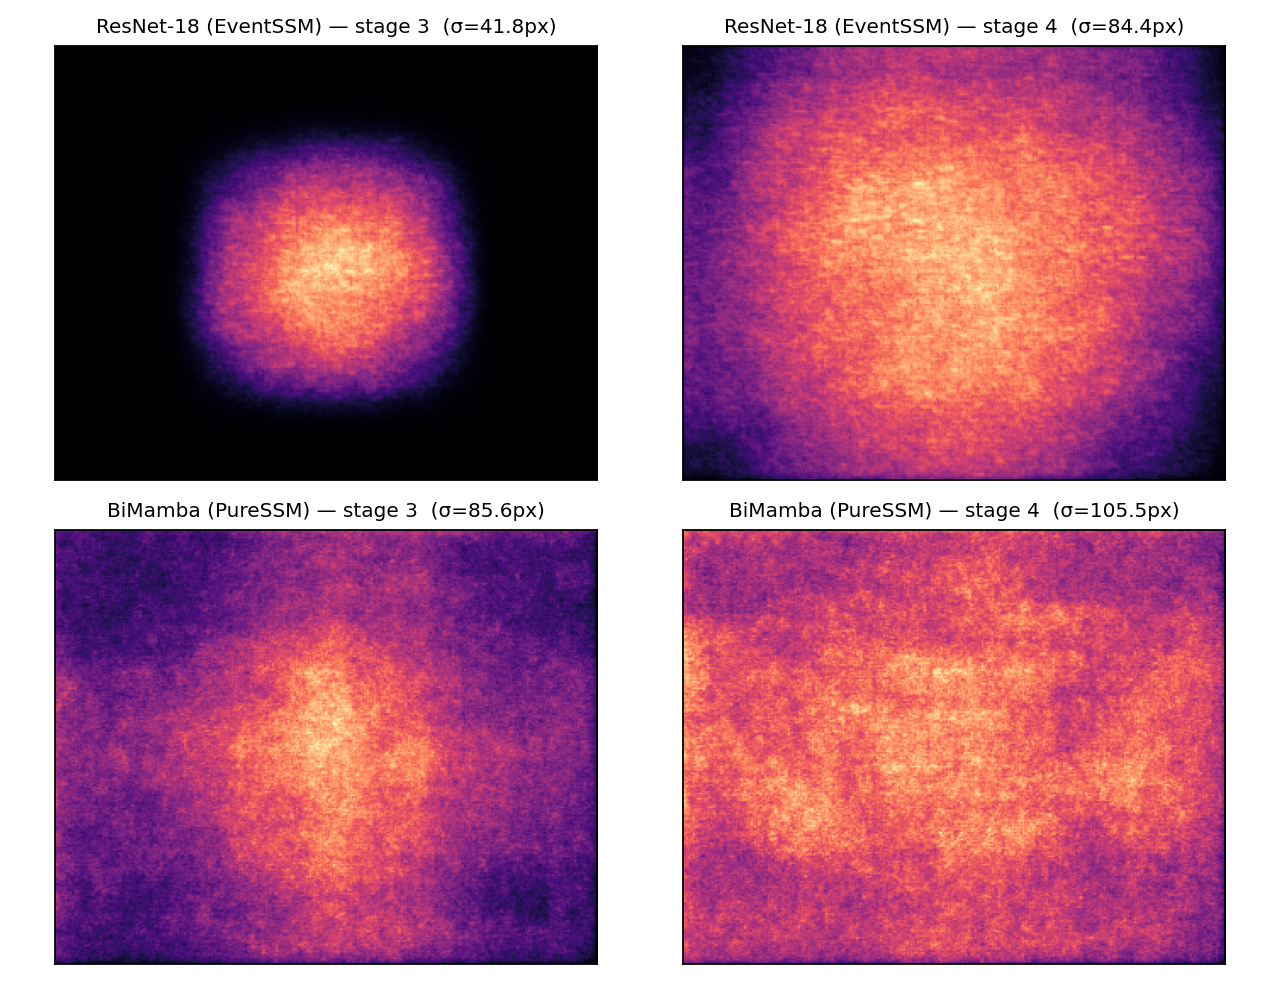
\includegraphics[width=0.85\textwidth]{images/fig_erf_trained.png}
    \caption[Receptive fields of the trained backbones]{Which input pixels influence the centre of the image in each trained backbone (brighter: more influence).
        $\sigma$ measures the spread. The state space backbone (BiMamba) draws on a wider area.}
    \label{fig:erf}
\end{figure}

\begin{table}[htbp]
\centering
\caption[Receptive field size by stage]{How wide an area of the image each backbone draws on ($\sigma$, in pixels), and how much training widened
    it.}
\label{tab:erf}
\begin{tabular}{lccc}
\toprule
\textbf{Backbone} & \textbf{Stage 3 $\sigma$} & \textbf{Stage 4 $\sigma$} & \textbf{$\Delta$ from training} \\
\midrule
ResNet-18 (EventSSM) & 41.8\,px & 84.4\,px & $+0.2$ / $+6.2$ \\
BiMamba (PureSSM)    & \textbf{85.6\,px} & \textbf{105.5\,px} & $\mathbf{+34.4}$ / $\mathbf{+30.1}$ \\
\bottomrule
\end{tabular}
\end{table}

\FloatBarrier
\section{Temporal Robustness}
\label{sec:robustness}
\subsection{True Event-Rate Change}
Table~\ref{tab:regime2} and Figure~\ref{fig:robustness} show what happens when frames really arrive faster.
At twice the normal rate, the three state space models keep about 95\,\% of their accuracy. At ten times the
rate, with a new frame every 5~ms and no retraining, S5-RVT keeps 62.2\,\% and EventSSM 63.0\,\%. PureSSM
keeps 69.7\,\%, the most of the state space models. RVT's original ConvLSTM model, tested in the same way,
keeps more than any of them, 97.7\,\% at twice and 80.3\,\% at ten times the rate. At ten times the rate it
scores 37.84~mAP, against 32.38 for PureSSM.  EventSSM and PureSSM process time in exactly
the same way, so PureSSM's extra robustness is linked to its spatial mixer. Its wider view of the image is a
likely reason, because frames at ten times the rate contain very few events, but this was not tested
directly.

\begin{table}[htbp]
\centering
\caption[Accuracy when frames arrive faster]{Accuracy (mAP) when frames arrive faster than in training, without and with the
    published time-step correction. In brackets: share of the model's normal accuracy that is kept. Last row:
    values published by Zubi\'{c} et al.~\cite{zubic2024state}, not reproduced here. Normal-rate values use the test data
    rebuilt for this test and differ from Table~\ref{tab:accuracy} by at most 0.03.}
\label{tab:regime2}
\label{tab:dt_comp}
\small
\begin{tabular}{lcccc}
\toprule
 & \textbf{RVT (ConvLSTM)} & \textbf{S5-RVT} & \textbf{EventSSM} & \textbf{PureSSM} \\
\midrule
Normal rate (50\,ms)             & 47.14 & 47.69 & 46.20 & 46.45 \\
$2\times$ faster                 & 46.08 (97.7\,\%) & 45.37 (95.1\,\%) & 44.13 (95.5\,\%) & 44.53 (95.9\,\%) \\
$2\times$, with correction       & --- & 44.51 (93.3\,\%) & 43.67 (94.5\,\%) & 44.13 (95.0\,\%) \\
$10\times$ faster                & \textbf{37.84 (80.3\,\%)} & 29.67 (62.2\,\%) & 29.09 (63.0\,\%) & 32.38 (69.7\,\%) \\
$10\times$, with correction      & --- & 19.96 (41.9\,\%) & 20.18 (43.7\,\%) & 19.70 (42.4\,\%) \\
\midrule
$10\times$, published            & 8.35 (17.7\,\%) & 39.84 (83.5\,\%) & --- & --- \\
\bottomrule
\end{tabular}
\end{table}

\begin{figure}[htbp]
    \centering
    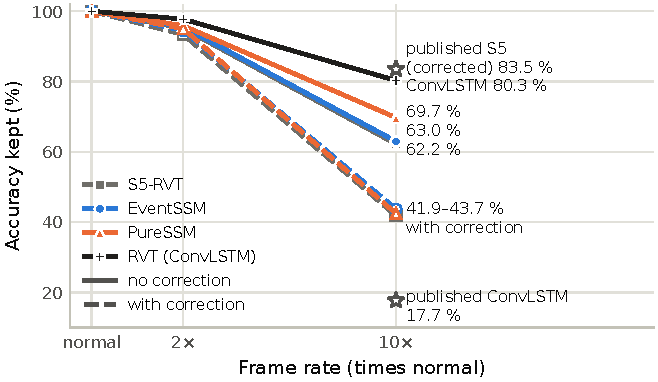
\includegraphics[width=0.8\textwidth]{images/fig_robustness_truerate.pdf}
    \caption[Robustness to faster frames]{Share of each model's normal accuracy that is kept when frames arrive
        faster. Dashed lines use the published correction. Stars: published values~\cite{zubic2024state}, not
        reproduced here.}
    \label{fig:robustness}
\end{figure}

\subsection{Reproducing Inference-Time \texorpdfstring{$\Delta$}{Delta}-Rescaling}
\label{subsec:f2}
Zubi\'{c} et al.~\cite{zubic2024state} report that state space detectors can handle event rates they were
not trained on if their step size $\Delta$ is adjusted at test time to match the new rate. With this
correction, they report 39.84~mAP for S5 at ten times the normal rate. This thesis applied the same
correction with the published code and model, and also to the two Mamba models (Table~\ref{tab:regime2}, row ``with correction'').
The correction lowered accuracy at every point tested. At ten times the rate it cost 9.7 points for
S5-RVT, 8.9 for EventSSM and 12.7 for PureSSM. The published 39.84 could not be reproduced with the
published code and model. The best S5-RVT result at ten times the rate was 29.67, without the correction.
The released code also cannot make test data at a faster frame rate, because its 50-ms step is fixed, so
the published experiment cannot be repeated exactly as released. The correction did not help in the window
test of Appendix~\ref{app:window} either. The robustness itself was reproduced. Without any correction, the
state space models keep 62 to 70\,\% of their accuracy. The other half of the published comparison was not.
The paper reports that RVT's ConvLSTM keeps only 17.7\,\% at ten times the rate, but tested on the same data
as the state space models it keeps 80.3\,\% (Table~\ref{tab:regime2}).

\section{Efficiency}
\label{sec:efficiency}
Table~\ref{tab:efficiency} compares the efficiency of the four non-spiking models.
PureSSM is the smallest model, needs the least computation and gives the most accuracy per unit of
computation. Yet it is the slowest in normal mode, at 26.86~ms per frame, or 37 frames per second. Its
spatial mixer consists of many small operations, and each operation on a GPU carries a fixed
start-up cost. In the faster CUDA-graph mode, most of this cost disappears, and PureSSM reaches 181 frames per
second. EventSSM is the fastest model, at 79 frames per second, and the faster of the two models run in the CUDA-graph mode, at 210. It also uses less
energy than the other state space models, 0.438~J per frame against 0.723~J for the baseline. RVT's
ConvLSTM, measured later with the same setup, puts these numbers in context. It is almost as fast as
EventSSM, at 76 frames per second, but it uses less than half of its energy, 0.169~J per frame. EventSSM's
speed and energy are therefore an advantage over the S5 baseline.

Sparsity does not make a GPU faster. Only
about 1.5\,\% of the input is non-zero (Section~\ref{sec:repr}), but every frame is still processed in
full. The Mamba models must keep 144.5~MB of memory for each video stream, 31 times the 4.7~MB of the
baseline and the ConvLSTM. This is because Mamba stores a large memory at every position in the image. On a small
platform with limited memory, this may be the figure that matters most.

\begin{table}[htbp]
\centering
\caption[Efficiency of the non-spiking models]{Size, computation, speed, energy and memory on one RTX 5070 Ti GPU, one frame at a time. Bold:
    best. The faster CUDA-graph mode was set up for the new models only. $^{\dagger}$Published
    model~\cite{gehrig2023recurrent}, measured later with the same setup (the other models, measured again
    then, agreed within 3.2\,\%).}
\label{tab:efficiency}
\begin{tabular}{lcccc}
\toprule
\textbf{Metric} & \textbf{RVT (ConvLSTM)}$^{\dagger}$ & \textbf{S5-RVT} & \textbf{EventSSM} & \textbf{PureSSM} \\
\midrule
Total parameters       & 18.54\,M & 18.19\,M & 19.18\,M & \textbf{16.33\,M} \\
FLOPs                  & 10.53\,G & 11.06\,G & 12.71\,G & \textbf{10.03\,G} \\
mAP per GFLOP          & 4.48 & 4.32 & 3.64 & \textbf{4.63} \\
Latency p50, eager     & 13.17\,ms & 17.14\,ms & \textbf{12.60\,ms} & 26.86\,ms \\
Throughput, eager      & 76\,Hz & 58\,Hz & \textbf{79\,Hz} & 37\,Hz \\
Throughput, CUDA-graph & --- & --- & \textbf{210\,Hz} & 181\,Hz \\
Energy per frame       & \textbf{0.169\,J} & 0.723\,J & 0.438\,J & 0.652\,J \\
Streaming state        & \textbf{4.7\,MB} & \textbf{4.7\,MB} & 144.5\,MB & 144.5\,MB \\
\bottomrule
\end{tabular}
\end{table}

\section{Example Detections}
\label{sec:qualitative}
Figure~\ref{fig:qualitative} shows eight evenly spaced frames from the test recording with the most large cars. The frames were not picked by hand. Four behaviours appear repeatedly across the recordings examined.
Close cars that produce events are detected with high confidence. Detections continue when the scene goes quiet. Even when almost no events fall on a car, both models keep detecting it, because the car is held in
the model's memory. At the start of a recording, when the memory is still empty, both models produce a few
weak boxes where there is no object. Finally, the labels themselves flicker and miss visible pedestrians,
so a correct detection can be counted as a mistake. The two models look very similar in these frames. The
difference between them rests on the measured scores of Section~\ref{sec:acc_results}.

\begin{figure}[htbp]
    \centering
    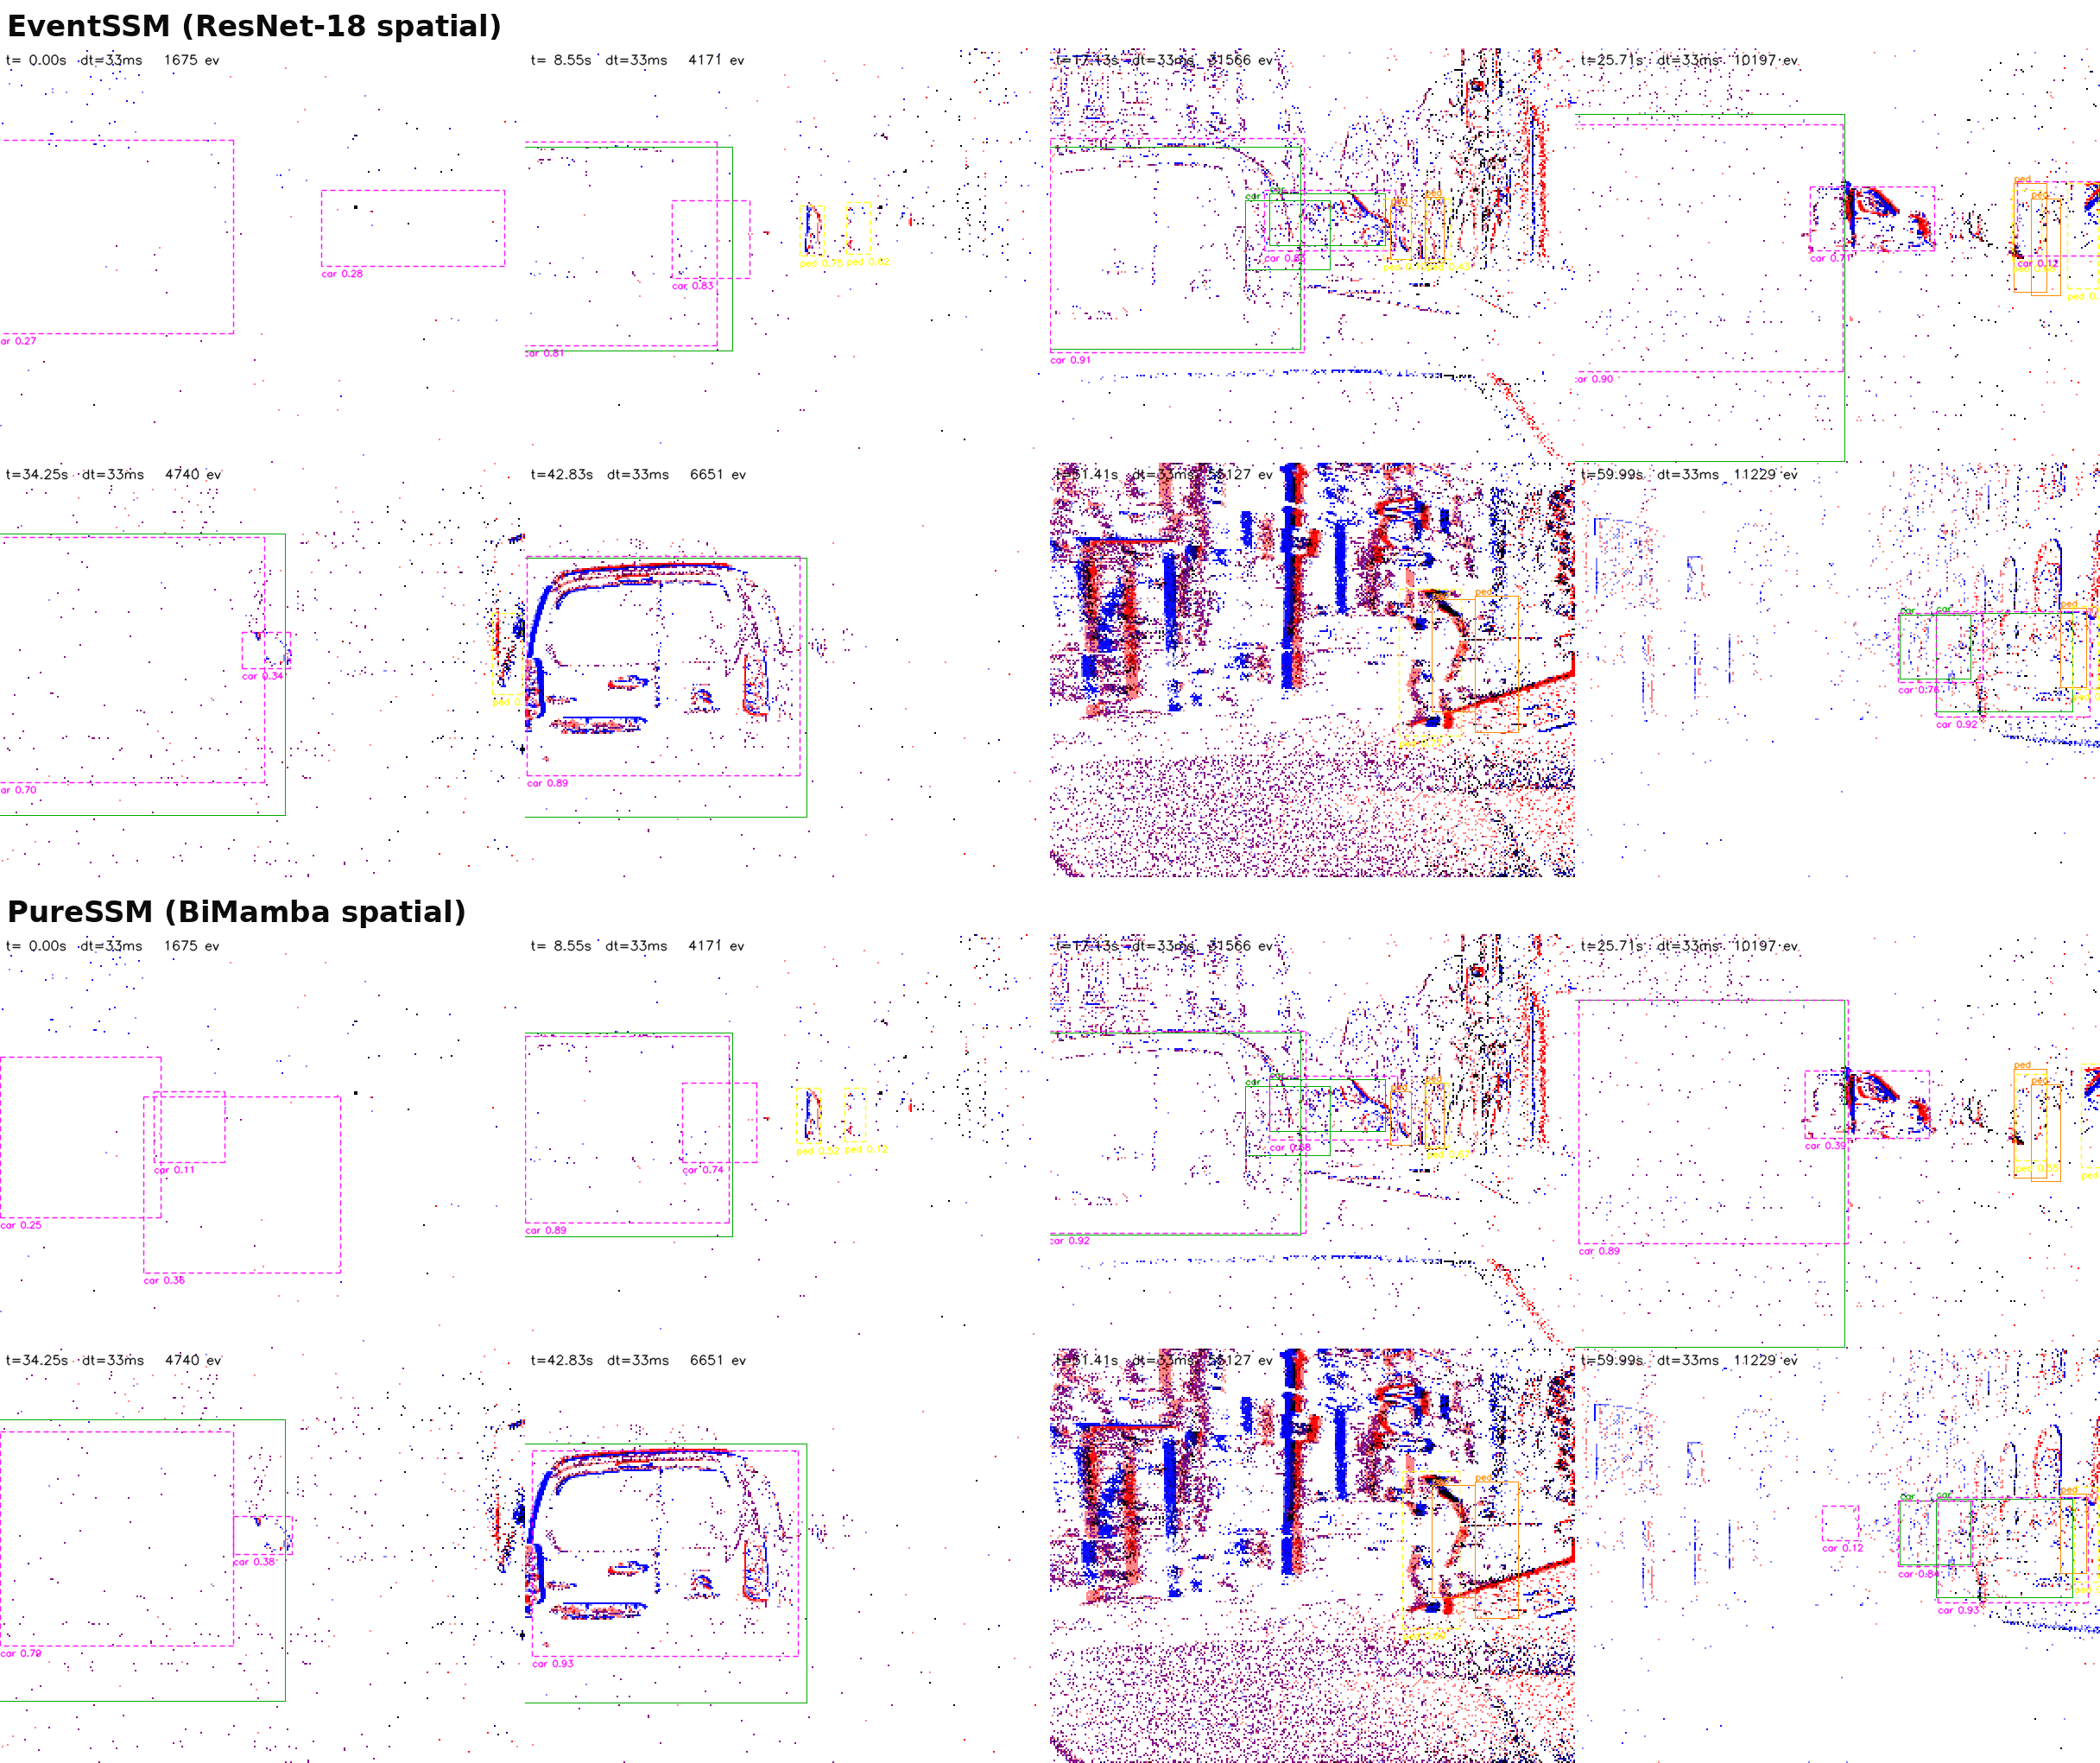
\includegraphics[width=\textwidth]{images/fig_qualitative_large_car.png}
    \caption[Ground truth and predictions on a large-car recording]{Eight evenly spaced frames from the test recording with the most large cars. Top: EventSSM; bottom: PureSSM.
        Solid boxes: ground truth (car green, pedestrian orange). Dashed boxes: predictions with confidence
        (car magenta, pedestrian yellow). Red and blue dots are events.}
    \label{fig:qualitative}
\end{figure}

\section{Spiking SSM Detector}
\label{sec:spiking_results}
The spiking model is a hybrid. Only its temporal readout spikes, and its spatial mixer is the same as
PureSSM's. It is therefore not directly comparable with the fully spiking detectors of
Table~\ref{tab:snn_landscape}, and its accuracy is context rather than a ranking. The main result of this
section is the breakdown of what spiking costs. The three readouts were trained on the short
100{,}000-step schedule and compared with a PureSSM trained on the same schedule. The graded readout was
also trained on the full schedule (Section~\ref{subsec:spk_full}).

\subsection{Accuracy and the Readout Ladder}
\label{subsec:spk_ladder}
\label{subsec:spk_accuracy}
On the short schedule, PureSSM scores 42.52~mAP, the analog readout 42.25, the graded readout 40.72 and the
spike readout, which sends binary spikes, 40.18 (Table~\ref{tab:spiking_ablation} and
Figure~\ref{fig:spiking_ladder}a). Turning the output into
binary spikes therefore costs 2.34 points in total, most of it on pedestrians. Figure~\ref{fig:spiking_ladder}b
splits this cost into the three steps of the ladder of Equation~\eqref{eq:ladder}. Adding the neuron's own
behaviour, its leak and reset, costs 0.28 points, with an interval from $-0.63$ to $+0.05$. Sparsity, with most outputs at zero, costs 1.52 points ($-1.98$ to $-1.06$). Reducing each signal to a single bit costs a further
0.54 points ($-1.07$ to $-0.07$). The order predicted before training (H4) therefore held. The last two steps
are clearly below zero, while the first is too small to measure on this test set. Sparsity is the largest cost, about three times the cost of the single bit. Because every readout is scored on the same
recordings, these step intervals, 0.7 to 1.0 points wide, are about four to six times narrower than the
interval of each single model (3.7 to 4.0 points, Table~\ref{tab:spiking_ablation}).

\begin{table}[htbp]
\centering
\caption[Accuracy of the spiking readouts (100k steps)]{The three spiking readouts and PureSSM, all trained for 100k steps (Gen1 test set). CI: 95\,\% confidence
    interval. Firing rate: share of readout outputs that are not zero.}
\label{tab:spiking_ablation}
\begin{tabular}{lccccc}
\toprule
\textbf{Model (100k steps)} & \textbf{mAP [95\,\% CI]} & \textbf{AP\textsubscript{50}} & \textbf{AP\textsubscript{L}} & \textbf{Car / Ped.} & \textbf{Firing rate} \\
\midrule
PureSSM (no LIF)   & 42.52 [40.40, 44.39] & 69.40 & 42.62 & 60.43 / 24.62 & n/a \\
analog (dense LIF) & 42.25 [40.14, 43.99] & 69.55 & 42.41 & 59.72 / 24.77 & 1.00 (dense) \\
graded             & 40.72 [38.66, 42.33] & 67.57 & 38.41 & 59.09 / 22.36 & 0.17 \\
spike (binary)     & 40.18 [38.09, 41.88] & 66.40 & 41.14 & 58.82 / 21.55 & 0.41 \\
\bottomrule
\end{tabular}
\end{table}

The single bit also slows down learning. The spike readout passes back only about a third of the learning
signal of the analog one, and during training it fell behind the graded readout only after about 60{,}000 steps
(Figure~\ref{fig:training_curves}). Its cost shrank as training went on, from 3.5 points in an early 25{,}000-step trial to 0.7 points on the validation set after 100{,}000 steps.

\begin{figure}[htbp]
    \centering
    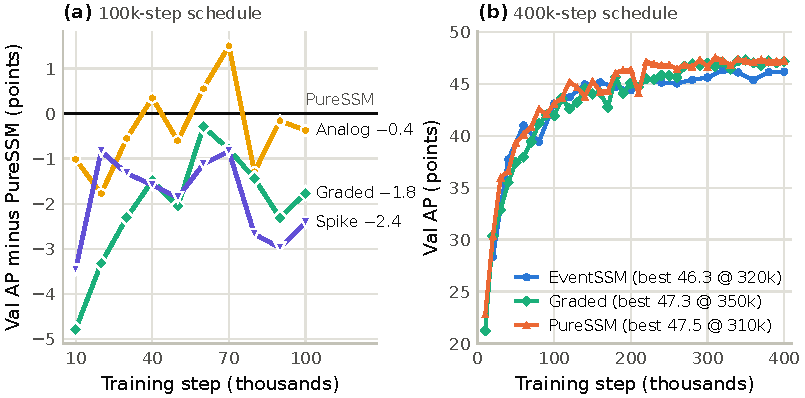
\includegraphics[width=\textwidth]{images/fig_training_curves.pdf}
    \caption[Validation mAP during training]{Validation accuracy during training. (a) The three spiking readouts minus PureSSM, all trained for 100k
        steps. (b) The 400k-step runs.}
    \label{fig:training_curves}
\end{figure}

\begin{figure}[htbp]
\centering
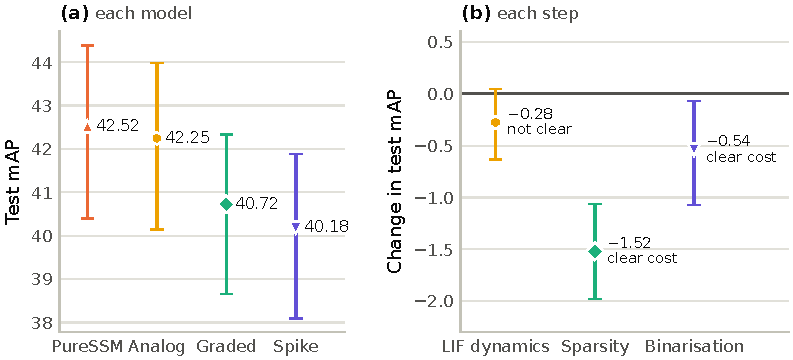
\includegraphics[width=\textwidth]{images/fig_ladder.pdf}
\caption[The cost of spiking, step by step]{The cost of spiking, step by step (100k-step models). (a) Accuracy of each model. (b) Change in accuracy at
    each step; a step whose interval does not cross zero is a clear cost. Intervals: 95\,\%. Those in (b)
    are narrower because each step compares the same test recordings.}
\label{fig:spiking_ladder}
\end{figure}

\subsection{The Graded Readout on the Full Schedule}
\label{subsec:spk_full}
Trained on the full schedule, the graded readout scores 46.24~mAP (Table~\ref{tab:accuracy}). This is only
0.19 below PureSSM, with an interval of $-0.66$ to $+0.09$ that includes zero, and level with EventSSM. On the
short schedule the same readout was 1.80 points behind PureSSM, so most of that loss came from learning more
slowly rather than from a lower final accuracy. On large objects it scores 49.63, the best of the new models.
That is 1.98 points above PureSSM, although the interval ($-0.40$ to $+3.59$) includes zero, and only 1.03
below the baseline. Training stayed stable (Figure~\ref{fig:training_400k}). The curves of the three full-schedule runs
overlap closely, even though the graded run was stopped and restarted three times, and on large objects the
graded run stays above the other two on the validation set over the last 100{,}000 steps. It took 55.5 hours on the desktop card, however, twice the 27.9 hours
of EventSSM, because the spatial scan and the neurons are slower to train.

\begin{figure}[htbp]
    \centering
    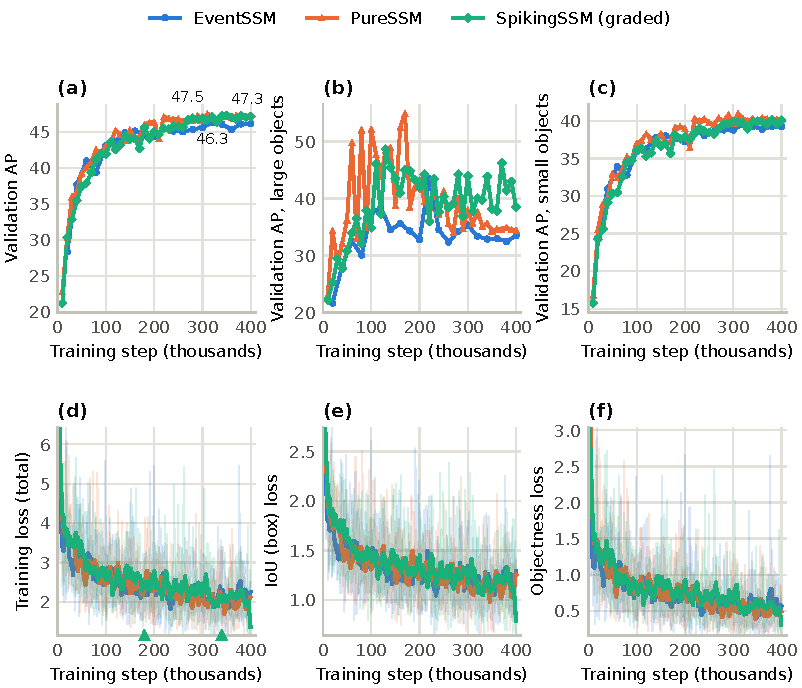
\includegraphics[width=0.9\textwidth]{images/fig_training_400k.pdf}
    \caption[Validation accuracy and training losses of the 400k-step runs]{The 400k-step runs during training: validation accuracy (a) overall, (b) on large and (c) on small objects;
        training losses (d)--(f). Triangles: points where the graded run was restarted.}
    \label{fig:training_400k}
\end{figure}

\subsection{Activity, Rate Robustness and Energy}
\label{subsec:spk_firing}
\label{subsec:spk_rate}
\label{subsec:spk_energy}
\label{subsec:spk_dynamics}
The readouts are active (non-zero) for only part of the time. On a test recording, the short-schedule graded readout is
active for 28, 13 and 10\,\% of its outputs at stages 2, 3 and 4, and the spike readout for 48, 36 and 39\,\%. During the short-schedule training
(Figure~\ref{fig:spiking_firing}), the activity of the spike readout rose at every stage, while that of the graded
readout fell at stages 3 and 4. The spike readout seems to make up for its single bit by firing more often.

\begin{figure}[htbp]
    \centering
    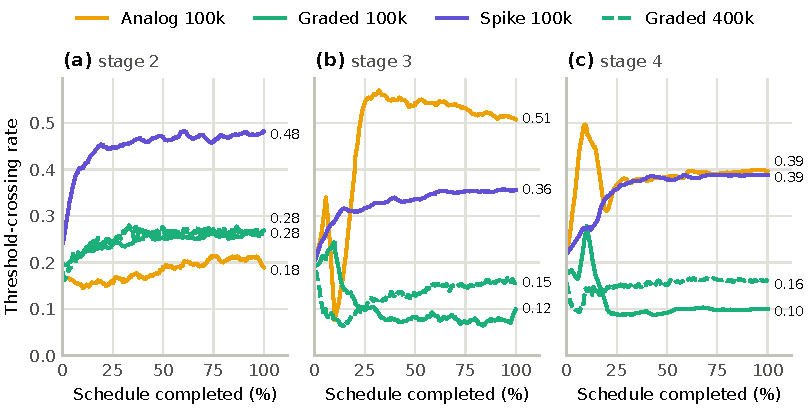
\includegraphics[width=\textwidth]{images/fig_spiking_firing.pdf}
    \caption[Readout firing rates during training]{How often the spiking readout fires during training, at stages (a) 2, (b) 3 and (c) 4. Solid: 100k-step
        runs; dashed: the graded 400k-step run.}
    \label{fig:spiking_firing}
\end{figure}

 Activity also hardly follows the scene.
Figure~\ref{fig:firing_pattern} follows both readouts through one minute of driving. Only stage~2 of the
graded readout becomes more active when the scene is busier, while the deeper stages fire at an almost
constant rate. Re-testing the
trained readouts with other firing thresholds showed that the training threshold gives the best accuracy. A higher threshold makes the neurons quieter but costs accuracy quickly.

\begin{figure}[htbp]
\centering
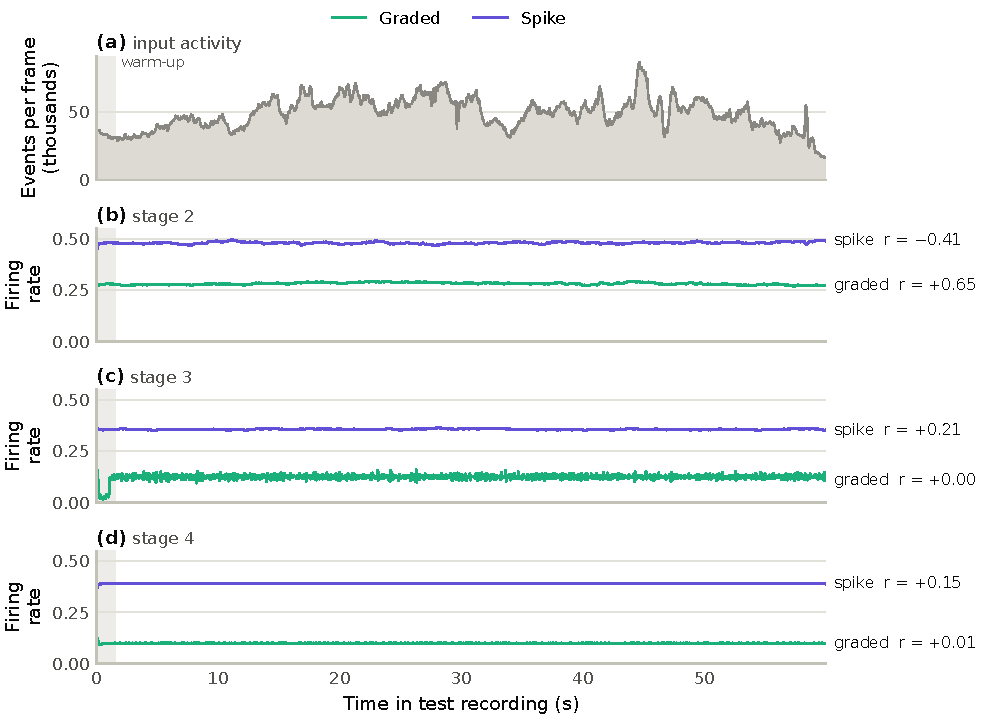
\includegraphics[width=\textwidth]{images/fig_firing_pattern.pdf}
\caption[Readout activity over one test recording]{Activity of the short-schedule readouts over one 60-s test recording. (a) Events per frame. (b)--(d) Firing rate (share of non-zero readout
    outputs) at stages 2--4; $r$: correlation with (a). Shaded: the first 32 frames, while the memory warms
    up (left out of $r$).}
\label{fig:firing_pattern}
\end{figure}

The readouts were also tested with frames arriving ten times faster, without correction. The graded readout
on the full schedule keeps 65.2\,\% of its accuracy, against 69.7\,\% for PureSSM. On the short schedule,
PureSSM keeps 69.1\,\%, the analog readout 67.6\,\%, the graded readout 63.2\,\% and the spike readout
70.3\,\%, slightly more than PureSSM on the same schedule. Sparsity therefore costs some robustness, and the single bit restores it. These are single runs, so differences of a few points are indicative only.

The energy that spiking could save is small. Equation~\eqref{eq:sop_energy} turns the measured activity into
an estimate. The graded readout on the full schedule would save 0.84\,\% of the energy per frame, and no
readout can save more than 1.04\,\%, because the spikes only feed 52.4 million of the 5.00 billion operations
per frame. The spike readout would save 0.96\,\%, slightly more, because an addition costs only about a fifth
of a multiply-add. The cost of moving data in memory, which is usually larger than the cost of the
arithmetic~\cite{horowitz2014computing}, is not included. On a GPU the spiking model brings no
saving at all. Every input is processed whether it is active or not, and the model is 0.73~ms per frame
slower than PureSSM. Chapter~\ref{ch:discussion} returns to these results
(Figures~\ref{fig:robustness_spiking} and~\ref{fig:threshold_sweep}). The other figures and tables are in
Appendix~\ref{sec:extra_spiking}.
\newpage
\section{Summary of Results}
\label{sec:results_summary}
The baseline was reproduced to within 0.01~mAP, which confirms the evaluation setup used for every other result.
Replacing the convolutional spatial mixer with a state space model left overall accuracy unchanged and
raised the large-object score by 2.95 points, a gain whose interval touches zero. The
receptive-field probe links it to a wider view of the image that the model learns in training. When frames
arrived ten times faster, the state space models kept 62 to 70\,\% of their accuracy without any correction,
PureSSM the most, while RVT's ConvLSTM kept 80\,\%. The published correction lowered accuracy instead, and
the published results could not be reproduced. EventSSM is the fastest model, PureSSM needs the least computation, and the ConvLSTM uses the least energy and memory. Finally,
most of the cost of spiking comes from sparsity rather than from the single bit. For the graded
readout this cost nearly disappears with full training, and the possible energy saving is at most about
1\,\%, because the spikes only reach the first layers of the neck.

\chapter{Discussion}
\label{ch:discussion}
This chapter interprets the results of Chapter~\ref{ch:results}. It first answers the research question and the four hypotheses. It then looks at what the state space mixer contributes, why the models cope with faster events, what efficiency really depends on, and how far the
path to neuromorphic hardware has come. It ends with the change of scope, the limitations of the work and the directions it opens.

\section{Answering the Research Question}
\label{sec:answer_rq}
The research question asked what the spatial mixer changes when everything else in the detector stays the same. Replacing a convolutional spatial mixer with a state space model keeps overall
accuracy the same. Its large-object score rises by 2.95 points, a gain whose interval touches zero. It also keeps more of its
accuracy than the other state space models when frames arrive faster, and it needs the least computation of
all the models tested. It is, however, the slowest model on a GPU in normal mode, and it carries 31 times more memory per video stream than the published models.

The second question asked what it costs to make the detector spike, and what spiking gives back. On the
short schedule, spiking costs 2.3 points, and most of that comes from sparsity. After full
training, the graded readout loses almost nothing. In this hybrid design, the estimated energy saving is at most about 1\,\%.

All six aims were met, with two qualifications. Efficiency was measured on a desktop GPU, not on the kind of computer a drone would carry, and the explanation of the large-object gain rests on a gain
whose interval touches zero.

Table~\ref{tab:hypotheses} sets each hypothesis against its outcome. H1 and H4 held, and H2 and H3 did not. H2 predicted that state space models would be more robust to the event rate than a ConvLSTM, and they were not. H3 predicted that the published correction would help, and it lowered accuracy instead. Section~\ref{sec:discuss_robustness} discusses what both results mean.

\begin{table}[htbp]
\centering
\small
\caption[The four hypotheses and their outcomes]{The four hypotheses of Section~\ref{sec:hypotheses} and what the
    experiments found.}
\label{tab:hypotheses}
\begin{tabularx}{\textwidth}{@{}l>{\raggedright\arraybackslash}X>{\raggedright\arraybackslash}X>{\raggedright\arraybackslash}p{2.3cm}@{}}
\toprule
 & \textbf{Prediction} & \textbf{Finding} & \textbf{Outcome} \\
\midrule
H1 & PureSSM detects large objects better than EventSSM & 2.95 points better (95\,\% interval $-0.09$ to $+6.35$);
     its view of the image is up to twice as wide & Supported, with a reservation \\
H2 & State space models lose less accuracy than a ConvLSTM when frames arrive faster & At ten times the rate
     they keep 62--70\,\%; the ConvLSTM keeps 80.3\,\% & Not supported \\
H3 & The published time-step correction makes them more robust & It costs 9--13 points at ten times the rate
     & Not supported \\
H4 & Accuracy: analog $\geq$ graded $>$ spike & 42.25, 40.72 and 40.18~mAP; both strict steps clearly below
     zero & Supported \\
\bottomrule
\end{tabularx}
\end{table}
\newpage

\section{What the State Space Model Contributes}
\label{sec:what_shown}
The first contribution is that a state space model can do more than follow events through time. It can also be the spatial backbone of an event-camera detector.

A convolution builds in the assumption that neighbouring pixels belong together, whereas a scan has no such assumption and must learn it from data. Even so, PureSSM, with no attention and almost no
convolution, matches the convolutional model on overall accuracy, with the fewest parameters and the least
computation of all the models.

PureSSM is, however, still 1.3 points behind the attention-based baseline.
It was also trained with half the baseline's batch size, so part of that gap may come from the training
settings rather than from the design.

The second contribution is an explanation of where the gain comes from. Figure~\ref{fig:acc_by_size} shows
the pattern. On small and medium objects, every new model sits close to the baseline. On large objects,
EventSSM falls six points behind. PureSSM halves that gap, and the graded spiking model, which shares
PureSSM's spatial mixer, closes most of it.

\begin{figure}[htbp]
    \centering
    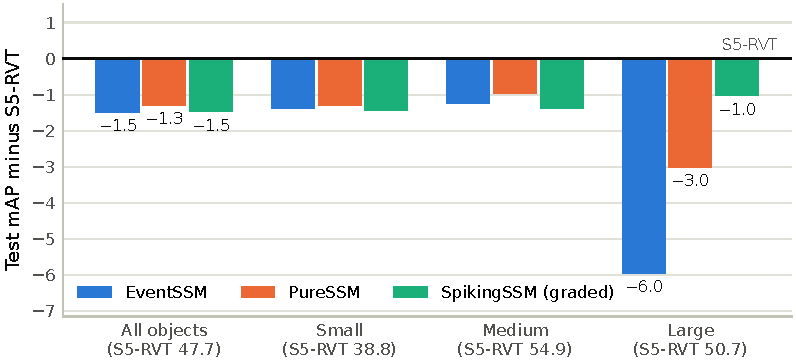
\includegraphics[width=0.75\textwidth]{images/fig_accuracy_by_size.pdf}
    \caption[Accuracy by object size, relative to S5-RVT]{Test mAP of the new models minus that of S5-RVT, overall and by object size; below zero is worse. On small
        and medium objects all models are close. On large objects PureSSM halves EventSSM's gap, and the
        spiking model's gap is the smallest.}
    \label{fig:acc_by_size}
\end{figure}

The receptive-field probe fits this pattern, because the state space mixer learns to draw on an area up to twice as wide as the convolutional one. The split by class agrees, since the
gain appears for cars, which are often large and close, and not for pedestrians. Each piece of evidence is
modest on its own, and the interval of the large-object gain touches zero, but the three agree.

Other published state space detectors keep a conventional method
for one of the two directions, attention for space in S5-RVT~\cite{zubic2024state}, or a ConvLSTM for time in
SMamba~\cite{yang2025smamba}. PureSSM shows that both directions can be handled by state space models. Where
raw speed on today's GPUs matters most, however, the convolutional EventSSM is still the better
choice.

\section{Temporal Robustness and the \texorpdfstring{$\Delta$}{Delta}-Rescaling Claim}
\label{sec:discuss_robustness}
Without the correction, all state space models kept between 62 and 70\,\% of their accuracy when frames
arrived ten times faster. Using the correction method published by Zubi\'{c} et al.~\cite{zubic2024state},
every model performed worse, by 9 to 13 points. The robustness was therefore already there, and it did not
come from the correction. A likely reason for these worse results, not tested here, is the size of the input.
The correction treats the input as a smooth signal that is simply sampled more often, where every sample is
as large as before.

Event frames act as counts. A 5-ms frame holds a tenth of the events of a 50-ms frame. Reducing the step
size $\Delta$ makes the memory fade at the right speed. It also cuts the weight with which each frame enters
the memory, again by a factor of ten. Without the correction, ten such frames add up to roughly one training
frame. With it, they add up to about a tenth of one. This means that the input to the memory over 50~ms
shrinks tenfold compared to training. That would also explain why the correction hurt all three models alike.
Under the correction, S5-RVT, EventSSM and PureSSM scored 19.96, 20.18 and 19.70~mAP.

Mamba's main feature, a step size that changes with the input, might be expected to help here. Its
advantage over S5 is small, however. EventSSM keeps 63.0\,\% against S5-RVT's 62.2\,\%, and the two models
also differ in their spatial mixers.

The ConvLSTM result differs most from the literature. Tested on the same data, it kept 80.3\,\% at ten times the rate, more
than any state space model, while the paper reports only 17.7\,\%. Robustness to the event rate is therefore not specific to state space models, since a ConvLSTM shows more of it. Why the ConvLSTM holds up better was not tested.

Figure~\ref{fig:robustness_spiking} follows the readout ladder at two and ten times the rate. At ten times the rate, the short-schedule PureSSM keeps 69.1\,\%, the analog readout 67.6\,\%, the graded readout 63.2\,\% and the spike readout 70.3\,\%. The leak and reset therefore cost a little robustness and sparsity costs more, while the spike readout keeps slightly more than PureSSM on the same schedule. A possible reason is that a binary spike always has the same size. When frames carry fewer
events, the spike readout loses some spikes, but each spike it keeps is as strong as before.

\begin{figure}[htbp]
    \centering
    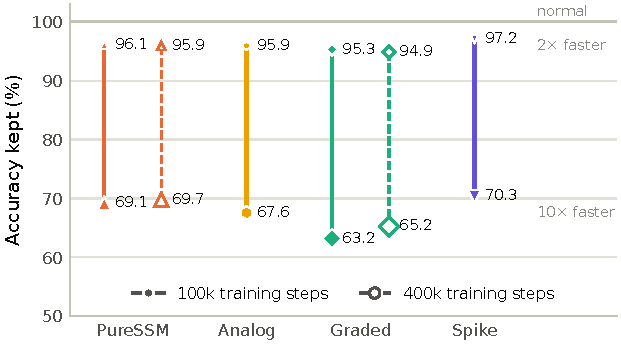
\includegraphics[width=0.75\textwidth]{images/fig_robustness_spiking.pdf}
    \caption[Rate robustness of the spiking readouts]{Share of normal accuracy kept when frames arrive 2 times (small marker) and 10 times faster (large marker),
        without correction. Filled: models trained for 100k steps; hollow: 400k steps. Single runs.}
    \label{fig:robustness_spiking}
\end{figure}

For a drone, whose event rate changes with its own speed, this means that all of these detectors lose accuracy gradually at rates they were never trained on, without any retuning.
The correction might behave differently with the unreleased code behind the published experiment, which cannot be checked with what was released.
\newpage
\section{Efficiency Trade-offs}
\label{sec:discuss_efficiency}
Table~\ref{tab:which_model} lists the best model for each limit a platform may have. Each model is best on a different measure, so the right choice depends on what matters most.

\begin{table}[htbp]
\centering
\small
\caption[The best model for each limit of the platform]{The best model for each limit a platform may have.}
\label{tab:which_model}
\begin{tabular}{@{}llll@{}}
\toprule
\textbf{Main limit} & \textbf{Best model} & \textbf{Value} & \textbf{Best new model} \\
\midrule
Accuracy             & S5-RVT          & 47.72 mAP        & PureSSM, 46.43 \\
Large objects        & S5-RVT          & 50.66 mAP        & SpikingSSM (graded), 49.63 \\
Faster frames        & RVT (ConvLSTM)  & 80.3\,\% kept    & PureSSM, 69.7\,\% \\
Model size           & PureSSM         & 16.33\,M parameters & PureSSM \\
Computation          & PureSSM         & 10.03 GFLOPs     & PureSSM \\
Speed                & EventSSM        & 12.60 ms per frame & EventSSM \\
Energy               & RVT (ConvLSTM)  & 0.169 J per frame & EventSSM, 0.438 J \\
Memory per stream    & RVT, S5-RVT     & 4.7 MB           & EventSSM, PureSSM: 144.5 MB \\
\bottomrule
\end{tabular}
\end{table}

Computation and speed disagree mostly for PureSSM. It needs the least computation, yet it is the
slowest model in normal mode. Figure~\ref{fig:efficiency} shows where its time goes. Most of it is spent in
the spatial mixer, which consists of many small operations, and each operation on a GPU carries a
fixed start-up cost. GPUs are also built for convolutions and run scans less efficiently.

\begin{figure}[htbp]
    \centering
    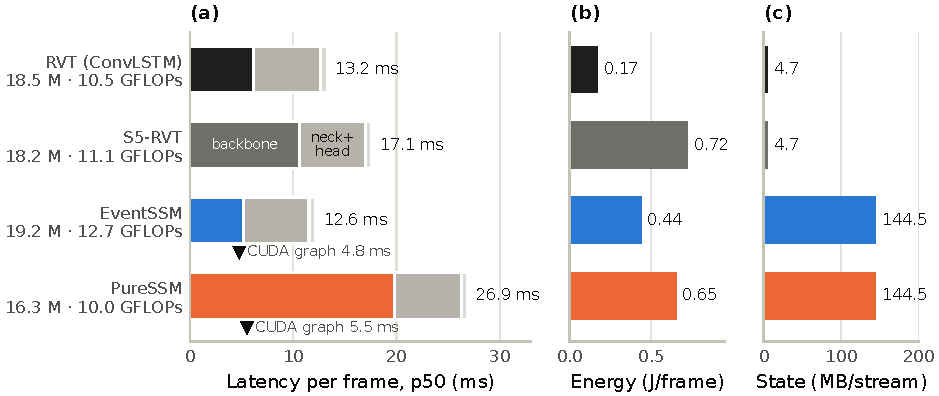
\includegraphics[width=\textwidth]{images/fig_efficiency.pdf}
    \caption[Efficiency of the non-spiking models]{Efficiency of the four non-spiking models (Table~\ref{tab:efficiency}). (a) Time per frame, split into its
        parts; the triangle marks the faster CUDA-graph mode. (b) Energy per frame. (c) Memory kept per
        video stream.}
    \label{fig:efficiency}
\end{figure}

The faster CUDA-graph  mode removes most of that start-up cost. It lifts PureSSM from 37 to 181 frames per
second, so much of the speed gap comes from the software, not from the method. Two costs remain all the
same. A GPU processes every pixel, so the sparsity of events, with only about 1.5\,\% of the input
non-zero, is never used. And the Mamba models carry 144.5~MB of memory per video stream, 31 times the 4.7~MB
of the published models.

Mamba keeps a large memory at every position of the image, which is
what lets it follow each position through time. On a desktop card, 144.5~MB hardly matters. On a small drone,
where several streams may share a limited memory, it could decide the choice of model. The ConvLSTM, by contrast, is fast, uses the least energy and memory, and was the most robust model as well, which makes it a strong candidate for deployment today.

\section{Latency and the Choice of Window}
\label{sec:latency_window}
Each event carries a time stamp precise to the microsecond, but the detectors in this thesis do not use that precision.

Every model collects events over 50-ms windows. Figure~\ref{fig:latency} splits the resulting delay into its
parts. An event waits 25~ms on average, and up to 50~ms, before its window closes. Processing then adds 13 to
27~ms. On average, the detector reacts 38 to 52~ms after an event, and it updates only 20 times per second,
like an ordinary video camera.

\begin{figure}[htbp]
    \centering
    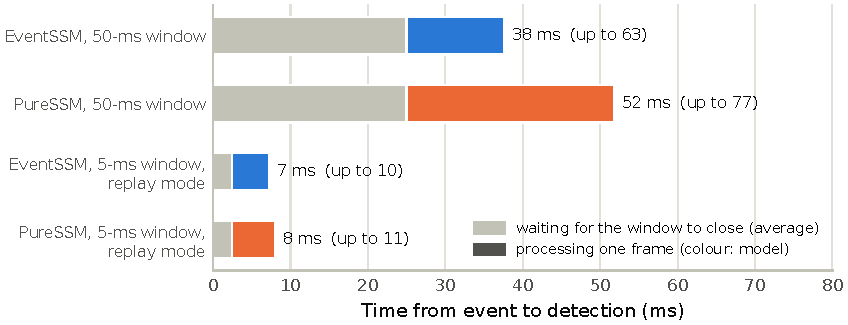
\includegraphics[width=0.85\textwidth]{images/fig_latency.pdf}
    \caption[Where the reaction time goes]{Time from an event to the detection that uses it, on average (worst case in
        brackets). Grey: waiting for the window to close. Colour: processing one frame. The 5-ms rows use the
        faster CUDA mode.}
    \label{fig:latency}
\end{figure}

The window length can be changed. With 5-ms windows and no retraining, the state space models keep
62 to 70\,\% of their accuracy. Processing must then finish within 5~ms. The normal mode cannot do this for either
new model. In the CUDA-graph mode, EventSSM just manages it, at 4.8~ms per frame, and PureSSM comes close, at
5.5~ms. The reaction time falls to about 7 to 8~ms.

Even with 50-ms windows, the camera keeps its other strengths, such as a very wide brightness range, no motion blur and a sparse output. Section~\ref{sec:future_work} discusses how the reaction time could be shortened.

\section{The Neuromorphic Deployment Path}
\label{sec:neuro_case}
The second research question asked what spiking costs and what neuromorphic hardware gives back.
Chapter~\ref{ch:results} answered the first half. This section takes up the second half. It covers what has been done towards running the detector on a neuromorphic chip, and what the results mean for that path.

\subsection{Why Neuromorphic Hardware}
Neuromorphic chips such as Intel's Loihi~2 only do work when a spike arrives, so their energy use follows
activity rather than the size of the input (Section~\ref{sec:neuromorphic_hw}). The state of the models in
this thesis suits them well. It breaks down into many small, independent parts, and each part can run as a
neuron.

Meyer et al.~\cite{meyer2024diagonal} ran a similar state on Loihi~2. When
inputs arrived one at a time, as they do from a streaming event camera, it used about 1000 times less energy
than on an NVIDIA Jetson board. If even part of that gain carried over to an event detector, it would matter
more to a small drone than any difference measured on a GPU.

\subsection{What Has Been Done}
This thesis deliberately separated the model from the chip. Hardware access depends on an agreement between
the university and Intel, and its timing was outside the project's control. The spiking model was
therefore built, trained and measured entirely in simulation, in a form chosen so that it can move to a chip
later. Table~\ref{tab:deploy} lists each part of the path, what was done and what is still missing.
\begin{table}[htbp]
\centering
\small
\caption[The neuromorphic deployment path: done and still needed]{Each part of the path from the simulated
    spiking model to a neuromorphic chip: what this thesis has done and what is still needed.}
\label{tab:deploy}
\begin{tabularx}{\textwidth}{@{}>{\raggedright\arraybackslash}p{2.9cm}>{\raggedright\arraybackslash}X>{\raggedright\arraybackslash}X@{}}
\toprule
\textbf{Part} & \textbf{Done in this thesis} & \textbf{Still needed} \\
\midrule
Spiking readout & Built, trained and measured; the graded mode matches Loihi~2's graded spikes
  & Export; lower-precision weights and states \\
Temporal memory & Trained; its step size changes with every input & A fixed-step version, retrained and compared \\
Memory size & Measured: 144.5~MB, about 37 million numbers per stream & A memory about 31 times smaller, as the 4.7~MB of RVT and S5-RVT \\
Reference version & NumPy version of one spiking temporal block that loads the trained weights; its own tests pass
  & Comparison with the trained model; checking an export against it \\
Spatial mixer, neck and head & Non-spiking; run on the GPU
  & A conventional processor next to the chip, or a spiking redesign \\
Energy & Estimated from operation counts: at most 1.04\,\% saved & Measurement on the chip \\
Hardware access & Two-page INRC proposal prepared with the supervisor (virtual lab first)
  & An agreement between UNSW and Intel, then hardware \\
Software & Lava discontinued; NIR chosen as the export format & The export itself; a supported Loihi software stack \\
\bottomrule
\end{tabularx}
\end{table}

Four pieces of work were done towards the chip. First, the readout was designed around the hardware. Its graded mode
carries a value with each spike, as Loihi~2's graded spikes do~\cite{orchard2021efficient}, so it can be
mapped to the chip without changing what the model computes.

Second, the activity of the readouts and the operations it drives were measured. This turns the energy
question into a number that a measurement on a chip can later confirm or deny.

Third, a reference version of one spiking temporal block was written in NumPy, without any deep-learning
library. It runs one time step at a time, as a chip would, and it loads the trained weights. Its own tests
pass.

Fourth, a two-page proposal to the Intel Neuromorphic Research Community was prepared for Will Midgley.
It asks for access to Intel's virtual lab first, and to hardware later.

The software ground also moved during the project. Intel discontinued its Lava framework in May
2026~\cite{intel2026lava}, so the export format was changed to NIR, a vendor-neutral format that several
simulators and chips can read~\cite{pedersen2024neuromorphic}. 

\newpage
\subsection{What the Results Mean for the Path}

The graded readout on the full schedule is active for only
14 to 26\,\% of its outputs, so the temporal part of a chip version would do a fraction of the work of a
dense one. Sparsity was the most expensive step of the ladder on the short schedule, but with full training the graded readout lost almost nothing, so the sparsity that a chip needs costs little accuracy.

Graded spikes are the natural target, because after full training the graded readout matches PureSSM's accuracy and Loihi~2 supports graded spikes directly. The binary spike readout is an alternative. On the short schedule it kept slightly more accuracy at ten times the rate than PureSSM (70.3 against 69.1\,\%).

The neurons' leak stayed within 0.044 of its starting value in every channel, so a chip can use one fixed leak, which is the simplest case to implement.

The main obstacle is Mamba's changing step size. Mamba recomputes it from every input, and a neuron with a fixed decay cannot do that. The results suggest that giving it up may cost little. Mamba's robustness edge over S5 was under one percentage point, the robustness came from
the memory itself, and the most accurate model of this thesis, S5-RVT, uses a memory with a fixed step.
Whether a fixed-step memory works as well in this backbone has not been tested.

The memory must also shrink. Each video stream carries about 37 million stored numbers, and even if each number were held by one neuron, that would fill many chips. The smaller memory proposed in Section~\ref{sec:future_work} is therefore a precondition for a chip.

Finally, in this hybrid a chip would hold only the temporal memory and the readout. The spikes reach about 1\,\% of the detector's operations (Figure~\ref{fig:spike_fed_ops}),
so even a readout with no activity at all would save at most about 1\,\%.

\begin{figure}[htbp]
    \centering
    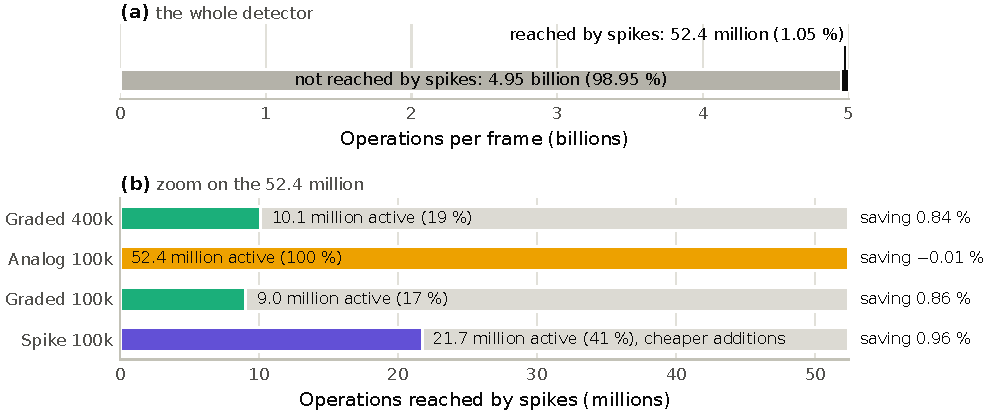
\includegraphics[width=\textwidth]{images/fig_spike_fed_ops.pdf}
    \caption[Share of operations reached by spikes]{How much of the detector's arithmetic the spikes reach. (a) All operations per frame: spikes reach only
        1.05\,\%. (b) Zoom on that 1.05\,\%: the share each readout drives and its estimated saving. Even a readout with no activity would save at most 1.04\,\%.}
    \label{fig:spike_fed_ops}
\end{figure}

Lowering the activity after training does not help either. Raising the firing threshold reduces
activity, but accuracy falls quickly (Figure~\ref{fig:threshold_sweep}). The quietest setting tested would
lift the estimated saving only from 0.86 to about 0.99\,\%, at a cost of 12.9 points. In a hybrid, features must also travel between a conventional processor and the chip at every frame, and moving data often
costs more energy than computing with it~\cite{horowitz2014computing}. Larger savings therefore require the spatial mixer to run on the chip as well.

\begin{figure}[htbp]
\centering
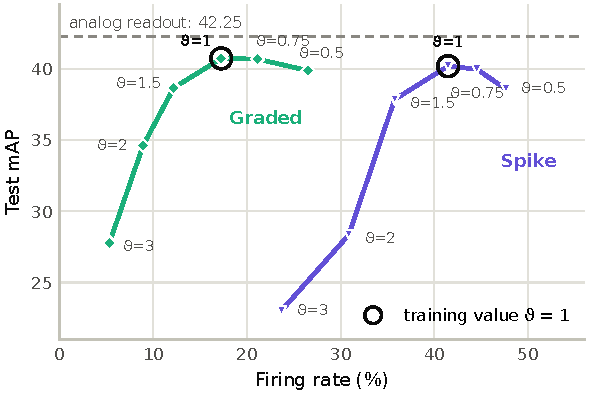
\includegraphics[width=0.75\textwidth]{images/fig_threshold.pdf}
\caption[Changing the firing threshold after training]{Changing the firing threshold after training (100k-step graded and binary readouts). Ringed point: the
    training value $\vartheta = 1$. Dashed line: the analog readout. Firing rate: share of the spike-fed
    operations that are active.}
\label{fig:threshold_sweep}
\end{figure}

\subsection{A Route to the Chip}
\label{subsec:route}
These findings suggest an order for the remaining work, from the cheapest and most informative step to the
most expensive:
\begin{enumerate}
  \item Replace Mamba's changing step size with a fixed one, retrain, and measure what is lost in accuracy
        and robustness. This needs only the desktop GPU.
  \item Shrink the memory until one stream fits on a few chips, and measure the cost again.
  \item Export the temporal block and the readout through NIR, and check the export frame by frame against
        the NumPy reference.
  \item Run the exported block in Intel's virtual lab, then on Loihi~2 hardware, and measure its energy and
        delay.
  \item Only then redesign the spatial mixer to spike, or to process only the parts of the image where
        events occur. That is where most of the energy is.
\end{enumerate}
A step that fails would still be informative, because it would show which property of the model a chip cannot support.

\section{Scope Change: the Obstacle-Avoidance Aim}
\label{sec:scope_change}
The fourth aim of Thesis~A was to connect the detector to an obstacle-avoidance controller, first in
simulation and then, if possible, on a real drone. This aim was removed from the scope, together with two
parts of the benchmarking aim, testing on the larger 1Mpx dataset and measuring speed on embedded hardware.
Table~\ref{tab:aims} compares every registered aim with what was delivered.

\begin{table}[htbp]
\centering
\small
\caption[Thesis A aims against what was delivered]{The aims registered in Thesis~A and what was delivered.}
\label{tab:aims}
\begin{tabularx}{\textwidth}{@{}l>{\raggedright\arraybackslash}X>{\raggedright\arraybackslash}X@{}}
\toprule
\textbf{Aim} & \textbf{Registered} & \textbf{Delivered} \\
\midrule
1 Architecture & SSM detector, comparing S4/S5/Mamba variants &
  Delivered: two Mamba detectors (EventSSM, PureSSM) and a spiking variant, compared against the S5
  baseline (Chapter~\ref{ch:method}). \\
2 Benchmarking & Gen1 and 1Mpx; accuracy, latency, memory, energy; CNN, RNN and transformer baselines;
  embedded-hardware latency &
  Delivered on Gen1 with all four metrics (Sections~\ref{sec:acc_results}, \ref{sec:efficiency}); the
  RNN baseline is RVT's published ConvLSTM checkpoint, measured for accuracy, rate robustness
  (Section~\ref{sec:robustness}) and efficiency (Section~\ref{sec:efficiency}) but not retrained;
  1Mpx deferred to future work (Section~\ref{sec:future_work}); latency and energy measured on a
  desktop GPU, not embedded hardware. \\
3 Temporal generalisation & Inference at frequencies other than training, without retraining &
  Delivered for frames arriving up to ten times faster, including a reproduction of inference-time
  $\Delta$-rescaling (Section~\ref{sec:robustness}; window-length test in Appendix~\ref{app:window}). \\
4 System integration & Obstacle-avoidance controller in simulation; micro-UAV flight if feasible &
  Descoped (this section). \\
\bottomrule
\end{tabularx}
\end{table}

The first reason was scientific. The detector is trained on Gen1, which was recorded from a car and only
contains cars and pedestrians. In a drone simulation, it would face objects and viewpoints it had never
seen. A collision rate measured there would mostly reflect that mismatch, together with the controller and
the simulator. It could not show what the backbone contributes, and that is the question of this thesis.

The second reason was practical. The aim depended on things outside the project's control, such as simulation tools
for event cameras, a stereo event camera that could not be integrated, drone hardware and flight approval. The time went into the controlled study instead. It produced the explanation of the large-object gain, the
robustness study and the efficiency comparison, none of which a simulated demonstration would have given.

\section{Limitations}
\label{sec:limitations}
\begin{table}[htbp]
\centering
\small
\caption[Limitations and their effect]{The limitations of this thesis, their effect on the conclusions and what would
    remove them.}
\label{tab:limitations}
\begin{tabularx}{\textwidth}{@{}>{\raggedright\arraybackslash}p{3.1cm}>{\raggedright\arraybackslash}X>{\raggedright\arraybackslash}X@{}}
\toprule
\textbf{Limitation} & \textbf{Effect on the conclusions} & \textbf{What would remove it} \\
\midrule
Single training runs & Differences below about one point cannot be read; the interval of the large-object gain touches zero
  & Three or more runs per model \\
One dataset (Gen1) & Findings may not hold for drones, night scenes or higher resolution
  & Training on 1Mpx and on drone-view data \\
Incomplete labels & Lower absolute scores, especially for pedestrians; comparisons unaffected
  & Denser, complete labels \\
Unequal starting points & EventSSM pre-trained, PureSSM not; published models trained differently
  & Retraining every model with one recipe \\
Desktop GPU & Speed and energy may differ on a drone's computer & Measuring on an embedded board \\
Narrow rate test & Only two and ten times faster, made from recorded events
  & Slower rates and truly fast scenes \\
Random-input probe & Receptive field measured without event data & Probing with real event frames \\
Spiking energy estimated & No measured saving; data movement ignored & Running the model on Loihi~2 \\
Spiking ladder on the short schedule & Only the graded readout was trained to the end
  & Full-length runs of all readouts \\
\bottomrule
\end{tabularx}
\end{table}

\textbf{Single training runs.} Each model was trained once. The bootstrap intervals show how much the scores
depend on which test recordings are used. They do not show how much a score would change if the same model
were trained again from a different random start, and that second source of variation is unknown here.
Neighbouring checkpoints of one run already differ by about 1.5 points on the validation set, which is why
differences below about one point are not treated as real.

The large effects, such as the 9 to 13 points lost to the correction, are well above this level, but the large-object gain, at 2.95 points with an interval that touches zero, is the result most at risk.

\textbf{One dataset, imperfect labels.} All results are on Gen1, recorded with a low-resolution camera of 304 by 240 pixels mounted on a car, with two classes and labels only about once per second. Many visible pedestrians
are not labelled at all, so a correct detection can count as a mistake. This lowers every model's score in
the same way, so the comparisons stand, but it limits what the absolute numbers mean. Whether the findings
hold for a drone's viewpoint, at night or at a higher resolution has not been tested.

\textbf{Unequal starting points.} The comparison between EventSSM and PureSSM is controlled, but not
perfectly. EventSSM's spatial mixer starts from weights pre-trained on photographs, while PureSSM's starts from
scratch. Pre-training usually helps, so this difference is more likely to have hidden a PureSSM advantage
than to have created one. The comparisons with the published models are looser still. The new models used a
smaller batch and lower numerical precision, and the ConvLSTM is RVT's published model, not one retrained
with these settings.

\textbf{A desktop graphics card.} Speed and energy were measured on one desktop card. A drone would carry a
small embedded computer, where the balance between convolutions and scans, and between computation and
memory, may well be different. The energy figures also come from the card's power above idle, which drifted
between runs. For the spiking model the drift was large enough that no energy difference is claimed.

\textbf{A narrow rate test.} Frames were only made to arrive two and ten times faster. A four-fold rate could
not be built, because Gen1's labels fall on a 250-ms grid that only allows certain window lengths, and longer windows were
tested only at the normal frame rate, in the window test of the appendix. The faster frames were also made by cutting
recorded events into shorter windows, not by recording faster scenes.

\textbf{The spiking model.} Its energy saving is an estimate from operation counts, priced with standard
figures for a 45-nm chip~\cite{horowitz2014computing}. It ignores the cost of moving data, which on real
hardware is often larger than the arithmetic. Only the graded readout was trained on the full schedule, so
the ladder itself rests on the short schedule. The firing threshold was fixed during training, and the
neurons' own leak hardly changed, so their memory was barely used.

\section{Future Research Opportunities}
\label{sec:future_work}
Table~\ref{tab:future} groups the directions for future work by how soon they could start.

\begin{table}[htbp]
\centering
\small
\caption[Directions for future research]{Directions for future research, by how soon they could start.}
\label{tab:future}
\begin{tabularx}{\textwidth}{@{}>{\raggedright\arraybackslash}p{3.6cm}>{\raggedright\arraybackslash}X>{\raggedright\arraybackslash}X@{}}
\toprule
\textbf{Direction} & \textbf{Question it answers} & \textbf{What it needs} \\
\midrule
\multicolumn{3}{@{}l}{\textbf{Near term}} \\
Repeat the training & Is the large-object gain real? & About 30 hours per run \\
Train across event rates & Can training replace the failed correction? & A change to the data loader \\
A smaller memory & How much memory does accuracy need? & Changes to the temporal block \\
Shorter windows, retrained & How fast can the detector react? & 5-ms training data \\
\midrule
\multicolumn{3}{@{}l}{\textbf{Medium term}} \\
Higher resolution (1Mpx) & Does the large-object advantage grow? & Cloud storage and GPUs \\
Embedded hardware & Do speed and energy hold on a drone's computer? & An embedded board \\
Drone data and flight & Does the detector help a drone avoid collisions? & Drone-view data, a controller \\
\midrule
\multicolumn{3}{@{}l}{\textbf{Long term}} \\
Neuromorphic hardware & How much energy does spiking really save? & Loihi~2 access, a fixed step size \\
Fully spiking design & Can the whole detector spike without losing accuracy? & A spiking spatial mixer \\
\bottomrule
\end{tabularx}
\end{table}

\subsection{Near Term: Existing Code and Data}
\textbf{Repeat the training.} Three runs per model would show how much each result depends on chance. They
would also settle whether the large-object gain is real. At about 30 hours per run on the desktop card, this
is the cheapest way to strengthen the conclusions.

\textbf{Train across event rates.} The correction failed, but the problem it was meant to solve remains, because a drone's event rate changes all the time. A simpler answer is to train with that variation. Mixing windows of
different lengths during training would show the memory many rates at once. The rate test of this thesis
could then measure the gain directly.

\textbf{A smaller memory.} The 144.5~MB per stream is the main cost of the Mamba models. Shrinking the memory
kept at each position, or keeping a memory only where events occur, could close much of the gap to the
4.7~MB of the published models. The open question is how much accuracy and robustness this would cost.

\textbf{Shorter windows, with retraining.} Without retraining, 5-ms windows keep 62 to 70\,\% of the
accuracy. Retraining on such windows would show how much of the rest can be recovered, and Figure~\ref{fig:latency} shows that the reaction time would fall from 38--52~ms to about 7 to 8~ms.

\subsection{Medium Term: New Data or Hardware}
\textbf{Higher resolution.} The 1Mpx dataset~\cite{perot2020learning} has about 12.6 times as many pixels as
Gen1. Training on it would show whether the large-object advantage grows with resolution, as the wider view
of the state space mixer suggests it should. Higher-resolution event cameras also produce more
noise~\cite{gehrig2022high}, so the models should be trained on the new data.
With over a terabyte of raw data, training on it needs rented storage and GPUs.

\textbf{Embedded hardware.} Measuring speed, energy and memory on an embedded board would turn the efficiency
results into a deployment decision. It would also show whether the CUDA-graph mode's advantage holds on smaller
chips.

\textbf{Drone data and flight.} Once a detector has been trained on event data recorded from a drone, it can
be connected to an avoidance controller, as in event-based obstacle avoidance~\cite{falanga2020dynamic}, and
judged by how often it avoids a collision. This is where the original aim of Thesis~A would return, now on a
sound footing.

\subsection{Long Term: New Hardware or Designs}
\textbf{Neuromorphic hardware.} Section~\ref{subsec:route} sets out the route from the simulated model to
Loihi~2. Its first steps, a fixed step size and a smaller memory, can start on the desktop card. Its last, a
measured saving in place of the estimate of this thesis, needs hardware access through the Intel Neuromorphic
Research Community.

\textbf{A fully spiking design.} Neurons whose state works like a state space memory, such as
SiLIF~\cite{fabre2025silif}, could make the whole time direction spike. Processing only the parts of the
image where events occur~\cite{yang2025smamba} could finally turn the sparsity of events into real savings.
The spiking ladder of this thesis shows that such designs should focus on keeping accuracy at low firing rates.

\chapter{Conclusion}
\label{ch:conclusion}
The aim of this thesis was to identify what a state space model architecture contributes to object detection
with an event-based camera. This was achieved by setting up a controlled experiment that used a fixed and
verified pipeline, the S5-RVT detector reproduced in Thesis~A. Previous work reported that state space models
are competitive and cope better with changes in event rate than other models. However, every published
comparison changed several components at once, making it difficult to identify the effect of state space
models on object detection.

It was shown that state space models can replace the convolutional layers of a spatial backbone, with
comparable accuracy, less computation, and probably better detection of large objects, which fits their wider
view of the image.

S5-RVT, the published baseline, was reproduced to within 0.01~mAP and remained the most accurate model, at 47.72~mAP
overall and 50.66 on large objects, with a small memory of 4.7~MB per stream. However, it used the most energy
of the four non-spiking models, 0.723~J per frame, and was the least robust to faster frames, keeping
62.2\,\% of its accuracy at ten times the rate. It remains the best choice when accuracy matters most.

EventSSM was identified as the fastest model. It processes a frame in 12.60~ms, and in 4.8~ms in the faster
CUDA-graph mode, which makes it the only model shown to keep up with 5-ms windows. However, it performs the
weakest on large objects, with an AP of 44.70, and needs the most computation, 12.71~GFLOPs per frame. This
model is key when processing speed matters most.

PureSSM is the smallest model, with only 16.33 million parameters, which makes it 10.2\,\% smaller than the
baseline. It still reaches a competitive overall mAP of 46.43, 1.3 points below the baseline, probably detects
large objects better than EventSSM, and has the best accuracy per GFLOP, even though it was trained with half
the baseline's batch size. It is the most robust state space model, retaining 69.7\,\% of its accuracy at ten
times the rate. Its costs are speed and memory. It is the slowest model in normal mode, at 26.86~ms per frame,
and like EventSSM it needs 144.5~MB of memory per stream.

SpikingSSM is set up as a baseline for future work on neuromorphic hardware. After full training, its graded
readout is level with PureSSM, at 46.24~mAP, and has the best large-object score of the new models, 49.63. On
the short schedule, however, spiking cost 2.3 points, mostly through sparsity, and training took twice as long
as for EventSSM. Its estimated energy saving is only about 1\,\%, because the spikes reach only the first
layers of the neck.

No single model was best on every measure, so the right choice depends on the main limit of the platform:
S5-RVT for accuracy, the ConvLSTM for energy and robustness, EventSSM for speed and PureSSM for size and
computation. The state space models did not show the advantage in rate robustness over a ConvLSTM that earlier
work reported, and the published time-step correction could not be reproduced. These conclusions rest on
single training runs on one driving dataset. The next steps are to repeat the training, to train on
higher-resolution and drone-view data, and to give the spiking model a smaller memory and a fixed step size so
that it can run on a neuromorphic chip.

% ===================================================================== BACK MATTER (roman, continuing)
\clearpage
\pagenumbering{roman}
\setcounter{page}{\value{frontmatterpages}}

\phantomsection\addcontentsline{toc}{chapter}{\bibname}
\bibliographystyle{ieeetr}
\bibliography{references}

\appendix

\chapter{Mathematical Formulations}
\label{app:maths}

\section{Continuous-Time SSM}
A state space model describes how a hidden state $h(t)\in\mathbb{R}^N$ changes over time in response to an
input $u(t)$, and how the output $y(t)$ is read from that state. The matrix $A$ controls how the state
evolves, $B$ how the input enters it, $C$ how the output is read, and $D$ passes part of the input straight
to the output. In all the models of this thesis, $A$ is diagonal, so each part of the state evolves on its
own:

\begin{align}
    h'(t) &= A h(t) + B u(t) \\
    y(t) &= C h(t) + D u(t)
\end{align}

\section{Discretisation}
To run on a computer, the model is converted into a step-by-step update with a step size $\Delta$. With
the zero-order hold, which assumes that the input stays constant during each step, the update takes the form below. S5 uses this form, and Mamba-2 uses the simpler $\overline{B}=\Delta B$ of
Equation~\eqref{eq:mamba2_state}. $\overline{A}$ sets how quickly the state fades in one step, and
$\overline{B}$ how strongly each input is written into it. For a small step, $\overline{B}\approx\Delta B$,
so shrinking the step also weakens every input. The step size
is the value that the correction tested in Section~\ref{subsec:f2} adjusts, and this side effect is
discussed in Section~\ref{sec:discuss_robustness}.

\begin{align}
    \overline{A} &= \exp(\Delta A) \\
    \overline{B} &= (\exp(\Delta A) - I) A^{-1} B
\end{align}

\begin{align}
    h_k &= \overline{A} h_{k-1} + \overline{B} u_k \\
    y_k &= C h_k + D u_k
\end{align}

\section{Mamba Selective Scan}
In Mamba~\cite{gu2023mamba}, the step size and the input and output matrices are not fixed. They are
computed from the current input $u_k$ at every step by learned projections, so the model can decide at each
moment how much to remember. The Mamba-2 version used in this thesis is given in
Equations~\eqref{eq:mamba2_state} and~\eqref{eq:mamba2_out}.

\begin{equation}
    \Delta_k = \operatorname{softplus}\!\left(W_\Delta u_k + b_\Delta\right), \qquad
    B_k = W_B\, u_k, \qquad C_k = W_C\, u_k,
\end{equation}
where $W_\Delta$, $b_\Delta$, $W_B$ and $W_C$ are learned, and the softplus keeps the step size positive.
Mamba-2 also passes $B_k$ and $C_k$ through a short convolution over time, which is left out here.

\section{Event Representations}
This section defines the input format used by every model, and the one that was planned in Thesis~A.

\subsection{Stacked Histogram}
\label{subsec:stacked_hist}
Each event $k$, with time $t_k$, position $(x_k, y_k)$ and polarity $p_k$, is placed into one of $B=10$ time
slices of its window, where $t_{\min}$ and $t_{\max}$ are the first and last event times in the window. The
events are then counted for each polarity, time slice and pixel, with each count capped at $c=10$. The
resulting 20 count images are stacked into one input and stored as small integers.

\begin{equation}
  b_k = \min\!\left(\left\lfloor B\,\frac{t_k - t_{\min}}{\max(t_{\max}-t_{\min},\,1)}\right\rfloor,\; B-1\right),
  \label{eq:sh_bin}
\end{equation}

\begin{equation}
  S_{p,b}(x,y) = \min\!\left(c,\; \sum_k \mathbb{1}[p_k=p]\,\mathbb{1}[b_k=b]\,\mathbb{1}[x_k=x]\,\mathbb{1}[y_k=y]\right).
  \label{eq:sh_count}
\end{equation}

\subsection{Voxel Grid}
The voxel grid planned in Thesis~A instead spreads each event over the two nearest time slices, weighted by
how close it is to each. Here $T$ is the window length, $t_k$ is measured from the start of the window and
$\delta$ is one at zero and zero elsewhere. The voxel grid was not used, because every model uses the stacked
histogram of the shared pipeline (Section~\ref{sec:repr}).

\begin{equation}
    V_b(x, y) = \sum_k p_k \cdot \max(0, 1 - |(B-1) \cdot t_k / T - b|) \cdot \delta(x-x_k) \cdot \delta(y-y_k)
\end{equation}

\chapter{Reproducibility}
\label{app:repro}
Everything needed to repeat the experiments is stored in the project repository. The exact software versions
are fixed in the \texttt{env/} folder (Table~\ref{tab:env}). Step-by-step guides in \texttt{docs/runbooks/}
explain how to set up a new computer, repeat the baseline reproduction and train on a rented GPU.

Two problems are documented there. The Mamba code must be installed
without letting the installer change other packages, because a default installation replaces PyTorch with
an incompatible version. Loading the trained models with recent versions of PyTorch also requires a specific
setting (\texttt{TORCH\_FORCE\_NO\_WEIGHTS\_ONLY\_LOAD=1}).

The original S5-RVT code is kept at a fixed version, and every change made to it is saved as a patch that
can be applied again. Every trained model behind a reported result is identified by a checksum in
Table~\ref{tab:ckpts}, and the exact settings of each model are stored with the code. The 573 automated
tests check that the code behaves as intended.

\begin{table}[htbp]
\centering
\small
\caption[Software environment]{Pinned software environment.}
\label{tab:env}
\begin{tabular}{ll}
\toprule
Component & Version \\
\midrule
Python & 3.11.15 \\
PyTorch & 2.11.0+cu128 (CUDA 12.8, Blackwell \texttt{sm\_120}) \\
\texttt{mamba-ssm} & 2.3.2.post1, built for \texttt{sm\_120} \\
\texttt{causal-conv1d} & 1.6.2.post1, built for \texttt{sm\_120} \\
PyTorch Lightning & 2.6.5 \\
Hydra & 1.3.2 \\
\texttt{torchdata} & 0.9.0 \\
Reference implementation & \texttt{ssms\_event\_cameras} at commit \texttt{7c871b5} \\
\bottomrule
\end{tabular}
\end{table}

\begin{table}[htbp]
\centering
\small
\caption[Checkpoints evaluated]{Model checkpoints behind the reported results (first 16 digits of the SHA-256 hash).}
\label{tab:ckpts}
\begin{tabular}{llll}
\toprule
Model & Origin & Selected step & SHA-256 (prefix) \\
\midrule
S5-RVT & published release~\cite{zubic2024state} & --- & \texttt{58396f15b6c6081c} \\
RVT (ConvLSTM) & published release~\cite{gehrig2023recurrent} & --- & \texttt{24ca76af9fc417ec} \\
EventSSM & run \texttt{8zotrwjw}, workstation & 320k (best val.) & \texttt{e94a36c2157bfea0} \\
PureSSM & run \texttt{aekvsalq}, rented RTX~5090 & 310k (best val.) & \texttt{a07c108b430d288a} \\
SpikingSSM, graded & run \texttt{a43jctgx}, workstation & 350k (best val.) & \texttt{48002509ee12cbe6} \\
\midrule
\multicolumn{4}{@{}l}{\textbf{Short schedule (100k steps, final checkpoint)}} \\
PureSSM & run \texttt{igk6myyb}, workstation & 100k & \texttt{24c5a6083cb3df3a} \\
Analog readout & run \texttt{sx14rpo8}, workstation & 100k & \texttt{76efec6fbf6ebf57} \\
Graded readout & run \texttt{rnak3sms}, workstation & 100k & \texttt{44de83533cff07f7} \\
Spike readout & run \texttt{5ykgl80y}, workstation & 100k & \texttt{dad067cda73f766a} \\
\bottomrule
\end{tabular}
\end{table}

\chapter{Project Timeline}
\label{app:timeline}
Table~\ref{tab:timeline} and Figure~\ref{fig:gantt} show the plan registered in Thesis~A, and
Figure~\ref{fig:gantt_actual} shows what actually happened, rebuilt from the history of the code. The main
change is that the planned simulation and drone-testing phases were replaced by the controlled study of the
backbones and by the spiking model (Section~\ref{sec:scope_change}).The training runs, shown in the bottom
row of Figure~\ref{fig:gantt_actual}, took most of the calendar time. Each full run lasted between one and
two days.

\begin{table}[htbp]
    \centering
    \caption[Planned timeline and milestones (Thesis A)]{Planned timeline and milestones, as registered in Thesis~A.}
    \label{tab:timeline}
    \renewcommand{\arraystretch}{1.4}
    \begin{tabularx}{\textwidth}{|l|X|l|}
        \hline
        \rowcolor[gray]{0.9} \textbf{Phase} & \textbf{Tasks} & \textbf{Timeline} \\ \hline
        Literature Review \& Foundations & Complete literature survey; identify optimal SSM variant and event representation. & Weeks 1--12 (Thesis A)  \\ \hline
        Architecture Design & Design SSM detection architecture; implement in PyTorch. & Weeks 13--16 (Thesis A/B)  \\ \hline
        Dataset Preparation & Download and preprocess Gen1/1Mpx datasets; implement data loaders. & Weeks 17--18 (Thesis B) \\ \hline
        Training \& Benchmarking & Train models; benchmark against baselines; ablation studies. & Weeks 18--22 (Thesis B)  \\ \hline
        Temporal Generalisation & Evaluate multi-frequency deployment; compare with RNN/Transformer. & Weeks 23--25 (Thesis B)\\ \hline
        Simulation Integration & Integrate with avoidance controller; evaluate in simulation. & Weeks 26--29 (Thesis B)\\ \hline
        Hardware Testing (if feasible) & Deploy on physical UAV platform; collect real-world results. & Weeks 30--33 (Thesis B/C)\\ \hline
        Thesis Writing & Complete thesis document; final revisions. & Weeks 34--40 (Thesis C)  \\ \hline
    \end{tabularx}
\end{table}

\begin{figure}[htbp]
    \centering
    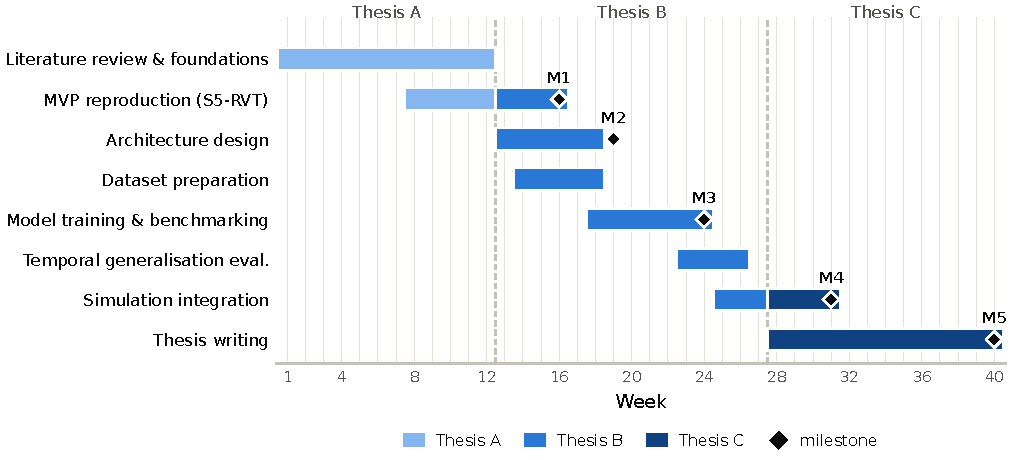
\includegraphics[width=\textwidth]{images/fig_gantt.pdf}
    \caption[Planned project timeline]{Planned schedule from Thesis~A, week by week; diamonds are milestones (M1--M5). Some week ranges differ from
        Table~\ref{tab:timeline}; both are shown as registered.}
    \label{fig:gantt}
\end{figure}

\begin{figure}[htbp]
    \centering
    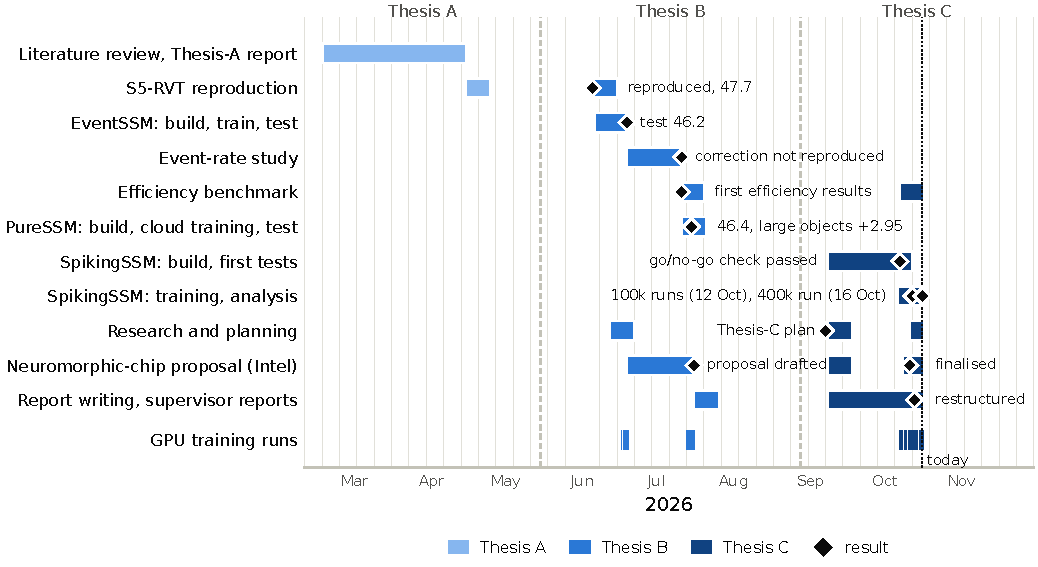
\includegraphics[width=\textwidth]{images/fig_gantt_actual.pdf}
    \caption[Project timeline as executed]{The project as it actually ran, February to November 2026, rebuilt from the code history for comparison with
        the plan in Figure~\ref{fig:gantt}. The literature review before the first commit is estimated.
        Bottom row: training runs. Diamonds: dated results. Colours: the three thesis terms, as in Figure~\ref{fig:gantt}.}
    \label{fig:gantt_actual}
\end{figure}

\chapter{Risk Assessment}
\label{app:risk}
Table~\ref{tab:risk_assessment} lists the main risks of Thesis~C, how likely and how serious each one was, how
it was handled and how it turned out by the end of the project.

\begin{table}[htbp]
    \centering
    \small
    \caption[Risk assessment]{Risk register for Thesis~C, with the outcome of each risk at the end of the project.}
    \label{tab:risk_assessment}
    \renewcommand{\arraystretch}{1.4}
    \begin{tabularx}{\textwidth}{|>{\RaggedRight\arraybackslash}p{3.2cm}|l|l|>{\RaggedRight\arraybackslash}X|}
        \hline
        \rowcolor[gray]{0.9} \textbf{Risk} & \textbf{Likelihood} & \textbf{Impact} & \textbf{Mitigation and outcome} \\ \hline
        Spiking model does not train stably & Medium & High & A stop rule was fixed before training: if the model was not training stably by 11~October, it would be frozen as a simulated proof of concept. Spiking was added one stage at a time. \textbf{Outcome:} passed on 7~October. All three readouts trained stably, and the graded readout completed the full schedule. \\ \hline
        Single training runs & High & Medium & Differences below about 1~mAP are not treated as findings, and paired bootstrap intervals give the uncertainty from the choice of test recordings. \textbf{Outcome:} remains the main limitation (Section~\ref{sec:limitations}). \\ \hline
        Training environment breaks & Medium & High & The hand-built software stack is pinned (Appendix~\ref{app:repro}), and guides and patches rebuild it from scratch. \textbf{Outcome:} an automatic system update removed the graphics driver twice, on 8~October and 12~November. It was reinstalled both times, and no run was affected. \\ \hline
        Long run lost to a crash & Medium & Medium & Training resumes from saved checkpoints, and a rented card of the same type is available as a fallback. \textbf{Outcome:} the graded runs were interrupted five times in total and resumed each time. Resuming restores the model and optimiser, but not the order of the training data. \\ \hline
        Test data lost & Low & Medium & The raw recordings and the scripts that build every derived data set are kept. \textbf{Outcome:} the faster-rate test data was deleted in October and rebuilt from the raw recordings before the final runs. \\ \hline
        Write-up completed late & Medium & High & Writing ran in parallel with the experiments, and the stop rule capped the time the spiking work could take. \textbf{Outcome:} the last experiments finished on 11~November, leaving the final weeks for writing. \\ \hline
        Neuromorphic hardware access delayed & High & Low & Hardware deployment was made future work, not a thesis result, and the model was built entirely in simulation. \textbf{Outcome:} Intel discontinued Lava in May~2026 and no hardware access was obtained during the project. The path to the chip is set out in Section~\ref{sec:neuro_case}. \\ \hline
    \end{tabularx}
\end{table}

\chapter{Additional Results}
\label{app:extra}
This appendix collects results that support Chapter~\ref{ch:results} but are not needed to follow it.

\section{Window-Length Test}
\label{app:window}
This test complements Section~\ref{sec:robustness}. The model still receives a frame every 50~ms, as in
training, but each frame collects events over a shorter or longer window, from 200 down to 12~ms. Only the
number of events in each frame changes, and the model's memory still takes one step every 50~ms. This is what
the published code of Zubi\'{c} et al.~\cite{zubic2024state} produces, because its 50-ms step is fixed.
Table~\ref{tab:regime1} shows that every model is most accurate at the 50-ms window it was trained on and
loses accuracy in both directions. At the 12-ms window, changing S5-RVT's step size with the published
correction, in either direction, lowered its accuracy from 38.4 to about 30~mAP. With the clock unchanged,
there is nothing for the correction to fix.

\begin{table}[htbp]
\centering
\caption[Robustness when the window length changes]{A frame every 50~ms, each collecting events over a shorter or longer window (mAP). Training used
    $1\times$. The $1\times$ values come from the rebuilt test data (Table~\ref{tab:accuracy}: 47.72, 46.22 and 46.43).}
\label{tab:regime1}
\begin{tabular}{llccc}
\toprule
\textbf{Multiplier} & \textbf{Window} & \textbf{S5-RVT} & \textbf{EventSSM} & \textbf{PureSSM} \\
\midrule
$0.25\times$ & 200\,ms & 40.95 & 40.90 & \textbf{41.65} \\
$0.5\times$  & 100\,ms & 46.48 & 45.54 & 45.67 \\
$1\times$    & 50\,ms  & 47.69 & 46.20 & 46.45 \\
$2\times$    & 25\,ms  & 45.04 & 43.52 & 44.09 \\
$4\times$    & 12\,ms   & 38.42 & 35.39 & 35.68 \\
\bottomrule
\end{tabular}
\end{table}

\section{Spiking Model}
\label{sec:extra_spiking}
Figure~\ref{fig:training_400k_time} shows the full-schedule runs against training time.

Table~\ref{tab:sop} gives the energy estimate of each readout, and Table~\ref{tab:spiking_bench} compares the
graded model with the non-spiking models on the graphics card.

\begin{figure}[htbp]
    \centering
    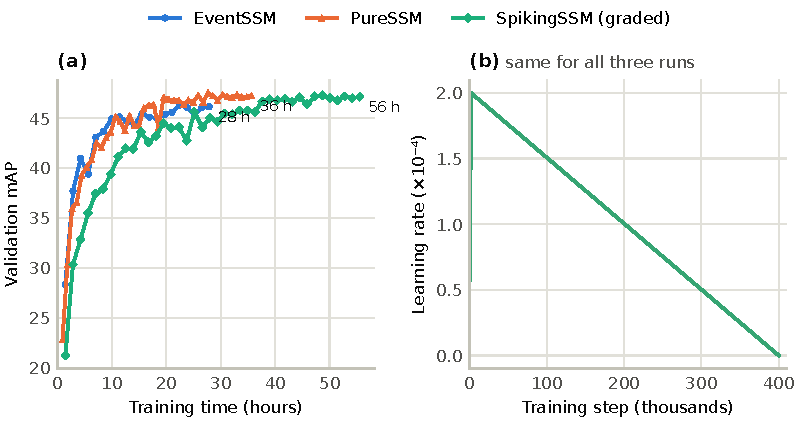
\includegraphics[width=\textwidth]{images/fig_training_400k_time.pdf}
    \caption[Validation mAP against training time]{(a) Validation accuracy against training hours; PureSSM trained on a faster rented graphics card, so its
        hours are not comparable. (b) The learning-rate schedule, the same for all three runs.}
    \label{fig:training_400k_time}
\end{figure}

\begin{table}[htbp]
\centering
\caption[Estimated energy saving per readout]{Estimated energy per frame from operation counts (Equation~\eqref{eq:sop_energy}). Nonzero rate: share of
    active readout outputs at stages 2, 3 and 4. Spikes reach only 52.4\,M of the 5.00\,G operations, so no
    readout can save more than 1.04\,\%.}
\label{tab:sop}
\small
\setlength{\tabcolsep}{3.5pt}
\begin{tabular}{lccccc}
\toprule
\textbf{Readout (priced as)} & \textbf{Nonzero rate, s2 / s3 / s4} & \textbf{Driven ops} & \textbf{mJ/frame} & \textbf{Dense} & \textbf{Saving} \\
\midrule
graded, 400k (MAC) & 0.263 / 0.140 / 0.157 & 10.1\,M & 22.81 & 23.01 & 0.84\,\% \\
analog, 100k (MAC) & 1.000 / 1.000 / 1.000 & 52.4\,M & 23.01 & 23.01 & $-0.01$\,\% \\
graded, 100k (MAC) & 0.257 / 0.125 / 0.100 & 9.0\,M & 22.81 & 23.01 & 0.86\,\% \\
binary, 100k (AC)  & 0.484 / 0.357 / 0.391 & 21.7\,M & 22.79 & 23.01 & 0.96\,\% \\
\bottomrule
\end{tabular}
\end{table}

\begin{table}[htbp]
\centering
\caption[Benchmark of the graded readout and the non-spiking models]{The graded spiking model and the non-spiking models, measured in one session; compare values within this
    table only. $^{*}$Idle power drifted; the range uses the idle power before and after the run.}
\label{tab:spiking_bench}
\begin{tabular}{lcccc}
\toprule
\textbf{Metric} & \textbf{S5-RVT} & \textbf{EventSSM} & \textbf{PureSSM} & \textbf{SpikingSSM, graded} \\
\midrule
Parameters              & 18.19\,M & 19.18\,M & 16.33\,M & 16.34\,M \\
FLOPs                   & 11.06\,G & 12.71\,G & 10.03\,G & 10.03\,G \\
Latency p50, full       & 16.93\,ms & 12.09\,ms & 26.46\,ms & 27.19\,ms \\
Latency p50, backbone   & 10.41\,ms & 5.19\,ms & 19.64\,ms & 20.30\,ms \\
Energy per frame (GPU)  & 0.701\,J & 0.43--0.52\,J$^{*}$ & 0.641\,J & 0.55--0.69\,J$^{*}$ \\
Streaming state         & 4.7\,MB & 144.5\,MB & 144.5\,MB & 145.6\,MB \\
\bottomrule
\end{tabular}
\end{table}

\end{document}
